\section{Exponentialfunktionen – Die Funktionen des Wachstums und Zerfalls}
\label{sec:exponentialfunktionen_intro}


\begin{aufgabenumgebung}{Erste Übungen mit $e^x$}
\begin{enumerate}
    \item Bilde die erste und zweite Ableitung der folgenden Funktionen:
        \begin{itemize}
            \item $f_1(x) = 3e^x - x^3 + 2x - 7$
            \item $f_2(x) = -0.5e^x + \frac{1}{x}$ (Tipp: $\frac{1}{x} = x^{-1}$)
        \end{itemize}
    \item Bestimme die Menge aller Stammfunktionen:
        \begin{itemize}
            \item $g_1(x) = 4e^x + 6x^2 - 1$
            \item $g_2(x) = \frac{e^x}{2} - \sqrt{x}$ (Tipp: $\frac{e^x}{2} = \frac{1}{2}e^x$)
        \end{itemize}
    \item Berechne das bestimmte Integral $\int_0^1 e^x \,dx$. Was stellt dieser Wert geometrisch dar?
\end{enumerate}
\end{aufgabenumgebung}

\begin{loesungsumgebung}[loes:erste-uebungen-ex]{Erste Übungen mit $e^x$}

\begin{enumerate}[label=(\alph*)]
    \item \textbf{Bilde die erste und zweite Ableitung der folgenden Funktionen:}
    \begin{itemize}
        \item \textbf{Funktion $f_1(x) = 3e^x - x^3 + 2x - 7$}
        \begin{itemize}
            \item Erste Ableitung $f_1'(x)$:
            $$ f_1'(x) = \frac{d}{dx}(3e^x - x^3 + 2x - 7) $$
            $$ f_1'(x) = 3\frac{d}{dx}(e^x) - \frac{d}{dx}(x^3) + \frac{d}{dx}(2x) - \frac{d}{dx}(7) $$
            $$ f_1'(x) = 3e^x - 3x^2 + 2 - 0 $$
            $$ \mathbf{f_1'(x) = 3e^x - 3x^2 + 2} $$
            \item Zweite Ableitung $f_1''(x)$:
            $$ f_1''(x) = \frac{d}{dx}(3e^x - 3x^2 + 2) $$
            $$ f_1''(x) = 3\frac{d}{dx}(e^x) - 3\frac{d}{dx}(x^2) + \frac{d}{dx}(2) $$
            $$ f_1''(x) = 3e^x - 3(2x) + 0 $$
            $$ \mathbf{f_1''(x) = 3e^x - 6x} $$
        \end{itemize}

        \item \textbf{Funktion $f_2(x) = -0.5e^x + \frac{1}{x}$} \\
        Wir schreiben $\frac{1}{x} = x^{-1}$. Also $f_2(x) = -0.5e^x + x^{-1}$.
        \begin{itemize}
            \item Erste Ableitung $f_2'(x)$:
            $$ f_2'(x) = \frac{d}{dx}(-0.5e^x + x^{-1}) $$
            $$ f_2'(x) = -0.5\frac{d}{dx}(e^x) + \frac{d}{dx}(x^{-1}) $$
            $$ f_2'(x) = -0.5e^x + (-1)x^{-1-1} $$
            $$ \mathbf{f_2'(x) = -0.5e^x - x^{-2}} \quad \text{oder} \quad \mathbf{-0.5e^x - \frac{1}{x^2}} $$
            \item Zweite Ableitung $f_2''(x)$:
            $$ f_2''(x) = \frac{d}{dx}(-0.5e^x - x^{-2}) $$
            $$ f_2''(x) = -0.5\frac{d}{dx}(e^x) - \frac{d}{dx}(x^{-2}) $$
            $$ f_2''(x) = -0.5e^x - (-2)x^{-2-1} $$
            $$ \mathbf{f_2''(x) = -0.5e^x + 2x^{-3}} \quad \text{oder} \quad \mathbf{-0.5e^x + \frac{2}{x^3}} $$
        \end{itemize}
    \end{itemize}

    \item \textbf{Bestimme die Menge aller Stammfunktionen:}
    \begin{itemize}
        \item \textbf{Funktion $g_1(x) = 4e^x + 6x^2 - 1$}
        \begin{align*} G_1(x) &= \int (4e^x + 6x^2 - 1) \,dx \\ &= 4\int e^x \,dx + 6\int x^2 \,dx - \int 1 \,dx \\ &= 4e^x + 6 \cdot \frac{x^3}{3} - x + C \\ &= \mathbf{4e^x + 2x^3 - x + C} \end{align*}

        \item \textbf{Funktion $g_2(x) = \frac{e^x}{2} - \sqrt{x}$} \\
        Wir schreiben $\frac{e^x}{2} = \frac{1}{2}e^x$ und $\sqrt{x} = x^{1/2}$. Also $g_2(x) = \frac{1}{2}e^x - x^{1/2}$.
        \begin{align*} G_2(x) &= \int \left(\frac{1}{2}e^x - x^{1/2}\right) \,dx \\ &= \frac{1}{2}\int e^x \,dx - \int x^{1/2} \,dx \\ &= \frac{1}{2}e^x - \frac{x^{\frac{1}{2}+1}}{\frac{1}{2}+1} + C \\ &= \frac{1}{2}e^x - \frac{x^{3/2}}{3/2} + C \\ &= \mathbf{\frac{1}{2}e^x - \frac{2}{3}x^{3/2} + C} \quad \text{oder} \quad \mathbf{\frac{1}{2}e^x - \frac{2}{3}\sqrt{x^3} + C} \end{align*}
    \end{itemize}

    \item \textbf{Berechne das bestimmte Integral $\int_0^1 e^x \,dx$. Was stellt dieser Wert geometrisch dar?}
    \begin{itemize}
        \item Eine Stammfunktion von $f(x)=e^x$ ist $F(x)=e^x$.
        \item Mit dem Hauptsatz der Differential- und Integralrechnung:
        $$ \int_0^1 e^x \,dx = [e^x]_0^1 = F(1) - F(0) = e^1 - e^0 $$
        Da $e^1=e$ und $e^0=1$, gilt:
        $$ \int_0^1 e^x \,dx = \mathbf{e - 1} $$
        (Numerischer Wert: $e-1 \approx 2.71828 - 1 = 1.71828$)
        \item \textbf{Geometrische Darstellung:} Der Wert $e-1$ stellt den \textbf{Flächeninhalt} dar, der vom Graphen der Funktion $f(x)=e^x$, der x-Achse, der y-Achse (Gerade $x=0$) und der Geraden $x=1$ eingeschlossen wird. Da die Funktion $e^x$ im Intervall $[0,1]$ stets positiv ist, entspricht das bestimmte Integral genau diesem Flächeninhalt.
    \end{itemize}
\end{enumerate}

\end{loesungsumgebung}

\begin{aufgabenumgebung}{Transformationen und Ableitungen/Stammfunktionen}
\begin{enumerate}
    \item Beschreibe, wie der Graph der Funktion $f(x) = 2e^{-0.5(x-1)} + 3$ aus dem Graphen der natürlichen Exponentialfunktion $y=e^x$ hervorgeht. Gib den Definitionsbereich, Wertebereich und die Gleichung der Asymptote an. Skizziere den Graphen.
    \item Bilde die erste Ableitung der folgenden Funktionen:
        \begin{itemize}
            \item $f_1(x) = 7e^{4x}$
            \item $f_2(x) = e^{-x} + 3x$
            \item $f_3(t) = A \cdot e^{-kt}$ ($A, k$ sind positive Konstanten; oft Modell für Zerfall)
        \end{itemize}
    \item Bestimme die Menge aller Stammfunktionen:
        \begin{itemize}
            \item $g_1(x) = 10e^{0.2x}$
            \item $g_2(x) = e^{-3x} - e^{2x}$
        \end{itemize}
\end{enumerate}
\end{aufgabenumgebung}


\begin{loesungsumgebung}[loes:trafo-ableitung-stammfunktion-ex]{Transformationen und Ableitungen/Stammfunktionen}

\begin{enumerate}[label=(\alph*)]
    \item \textbf{Beschreibung und Analyse von $f(x) = 2e^{-0.5(x-1)} + 3$}
    Der Graph der Funktion $f(x)$ geht aus dem Graphen der natürlichen Exponentialfunktion $y_0(u) = e^u$ durch folgende Transformationen hervor:
    \begin{enumerate}
        \item \textbf{Horizontale Skalierung/Spiegelung im Exponenten:} Der Exponent ist $-0.5(x-1) = -0.5x + 0.5$. Dies entspricht im Vergleich zu $e^x$:
        \begin{itemize}
            \item Einer Spiegelung an der y-Achse (wegen des negativen Vorzeichens vor dem $x$-Term).
            \item Einer horizontalen Streckung um den Faktor $1/0.5 = 2$.
            \item Einer horizontalen Verschiebung (die im Term $(x-1)$ bereits enthalten ist).
        \end{itemize}
        Alternativ kann man die Schritte so sehen:
        $e^x \xrightarrow{\text{Verschiebung um 1 nach rechts}} e^{x-1} \xrightarrow{\text{Horiz. Stauchung Faktor 0.5 + Spiegelung}} e^{-0.5(x-1)}$
        \item \textbf{Vertikale Streckung:} Multiplikation mit dem Faktor $2 \Rightarrow y_1(x) = 2e^{-0.5(x-1)}$. Der Graph wird in y-Richtung gestreckt.
        \item \textbf{Vertikale Verschiebung:} Addition von $3 \Rightarrow f(x) = 2e^{-0.5(x-1)} + 3$. Der Graph wird um 3 Einheiten nach oben verschoben.
    \end{enumerate}

    \begin{itemize}
        \item \textbf{Definitionsbereich ($D_f$):} Die Exponentialfunktion ist für alle reellen Zahlen definiert. Daher ist $\mathbf{D_f = \mathbb{R}}$.
        \item \textbf{Wertebereich ($W_f$):}
        Da $e^{\text{Exponent}}$ immer positiv ist ($e^{-0.5(x-1)} > 0$), ist $2e^{-0.5(x-1)} > 0$.
        Somit ist $f(x) = 2e^{-0.5(x-1)} + 3 > 3$.
        Der Wertebereich ist $\mathbf{W_f = (3, \infty)}$.
        \item \textbf{Gleichung der Asymptote:}
        Für $x \to \infty$: Der Exponent $-0.5(x-1)$ geht gegen $-\infty$. Daher $e^{-0.5(x-1)} \to 0$.
        Somit $\lim_{x \to \infty} f(x) = 2 \cdot 0 + 3 = 3$.
        Die Funktion hat eine \textbf{horizontale Asymptote} mit der Gleichung $\mathbf{y=3}$ (für $x \to \infty$).
        Für $x \to -\infty$: Der Exponent $-0.5(x-1)$ geht gegen $+\infty$. Daher $e^{-0.5(x-1)} \to \infty$.
        Somit $\lim_{x \to -\infty} f(x) = \infty$.
        \item \textbf{Skizze des Graphen:}
        Der Graph ist monoton fallend. Er nähert sich für $x \to \infty$ der Asymptote $y=3$ von oben an. Für $x \to -\infty$ wächst er unbegrenzt. Ein markanter Punkt ist $f(1) = 2e^0+3 = 2+3=5$, also $(1|5)$. Bei $x=0$ ist $f(0)=2e^{0.5}+3 \approx 2 \cdot 1.649 + 3 = 3.298+3 = 6.298$.
        \begin{center}
        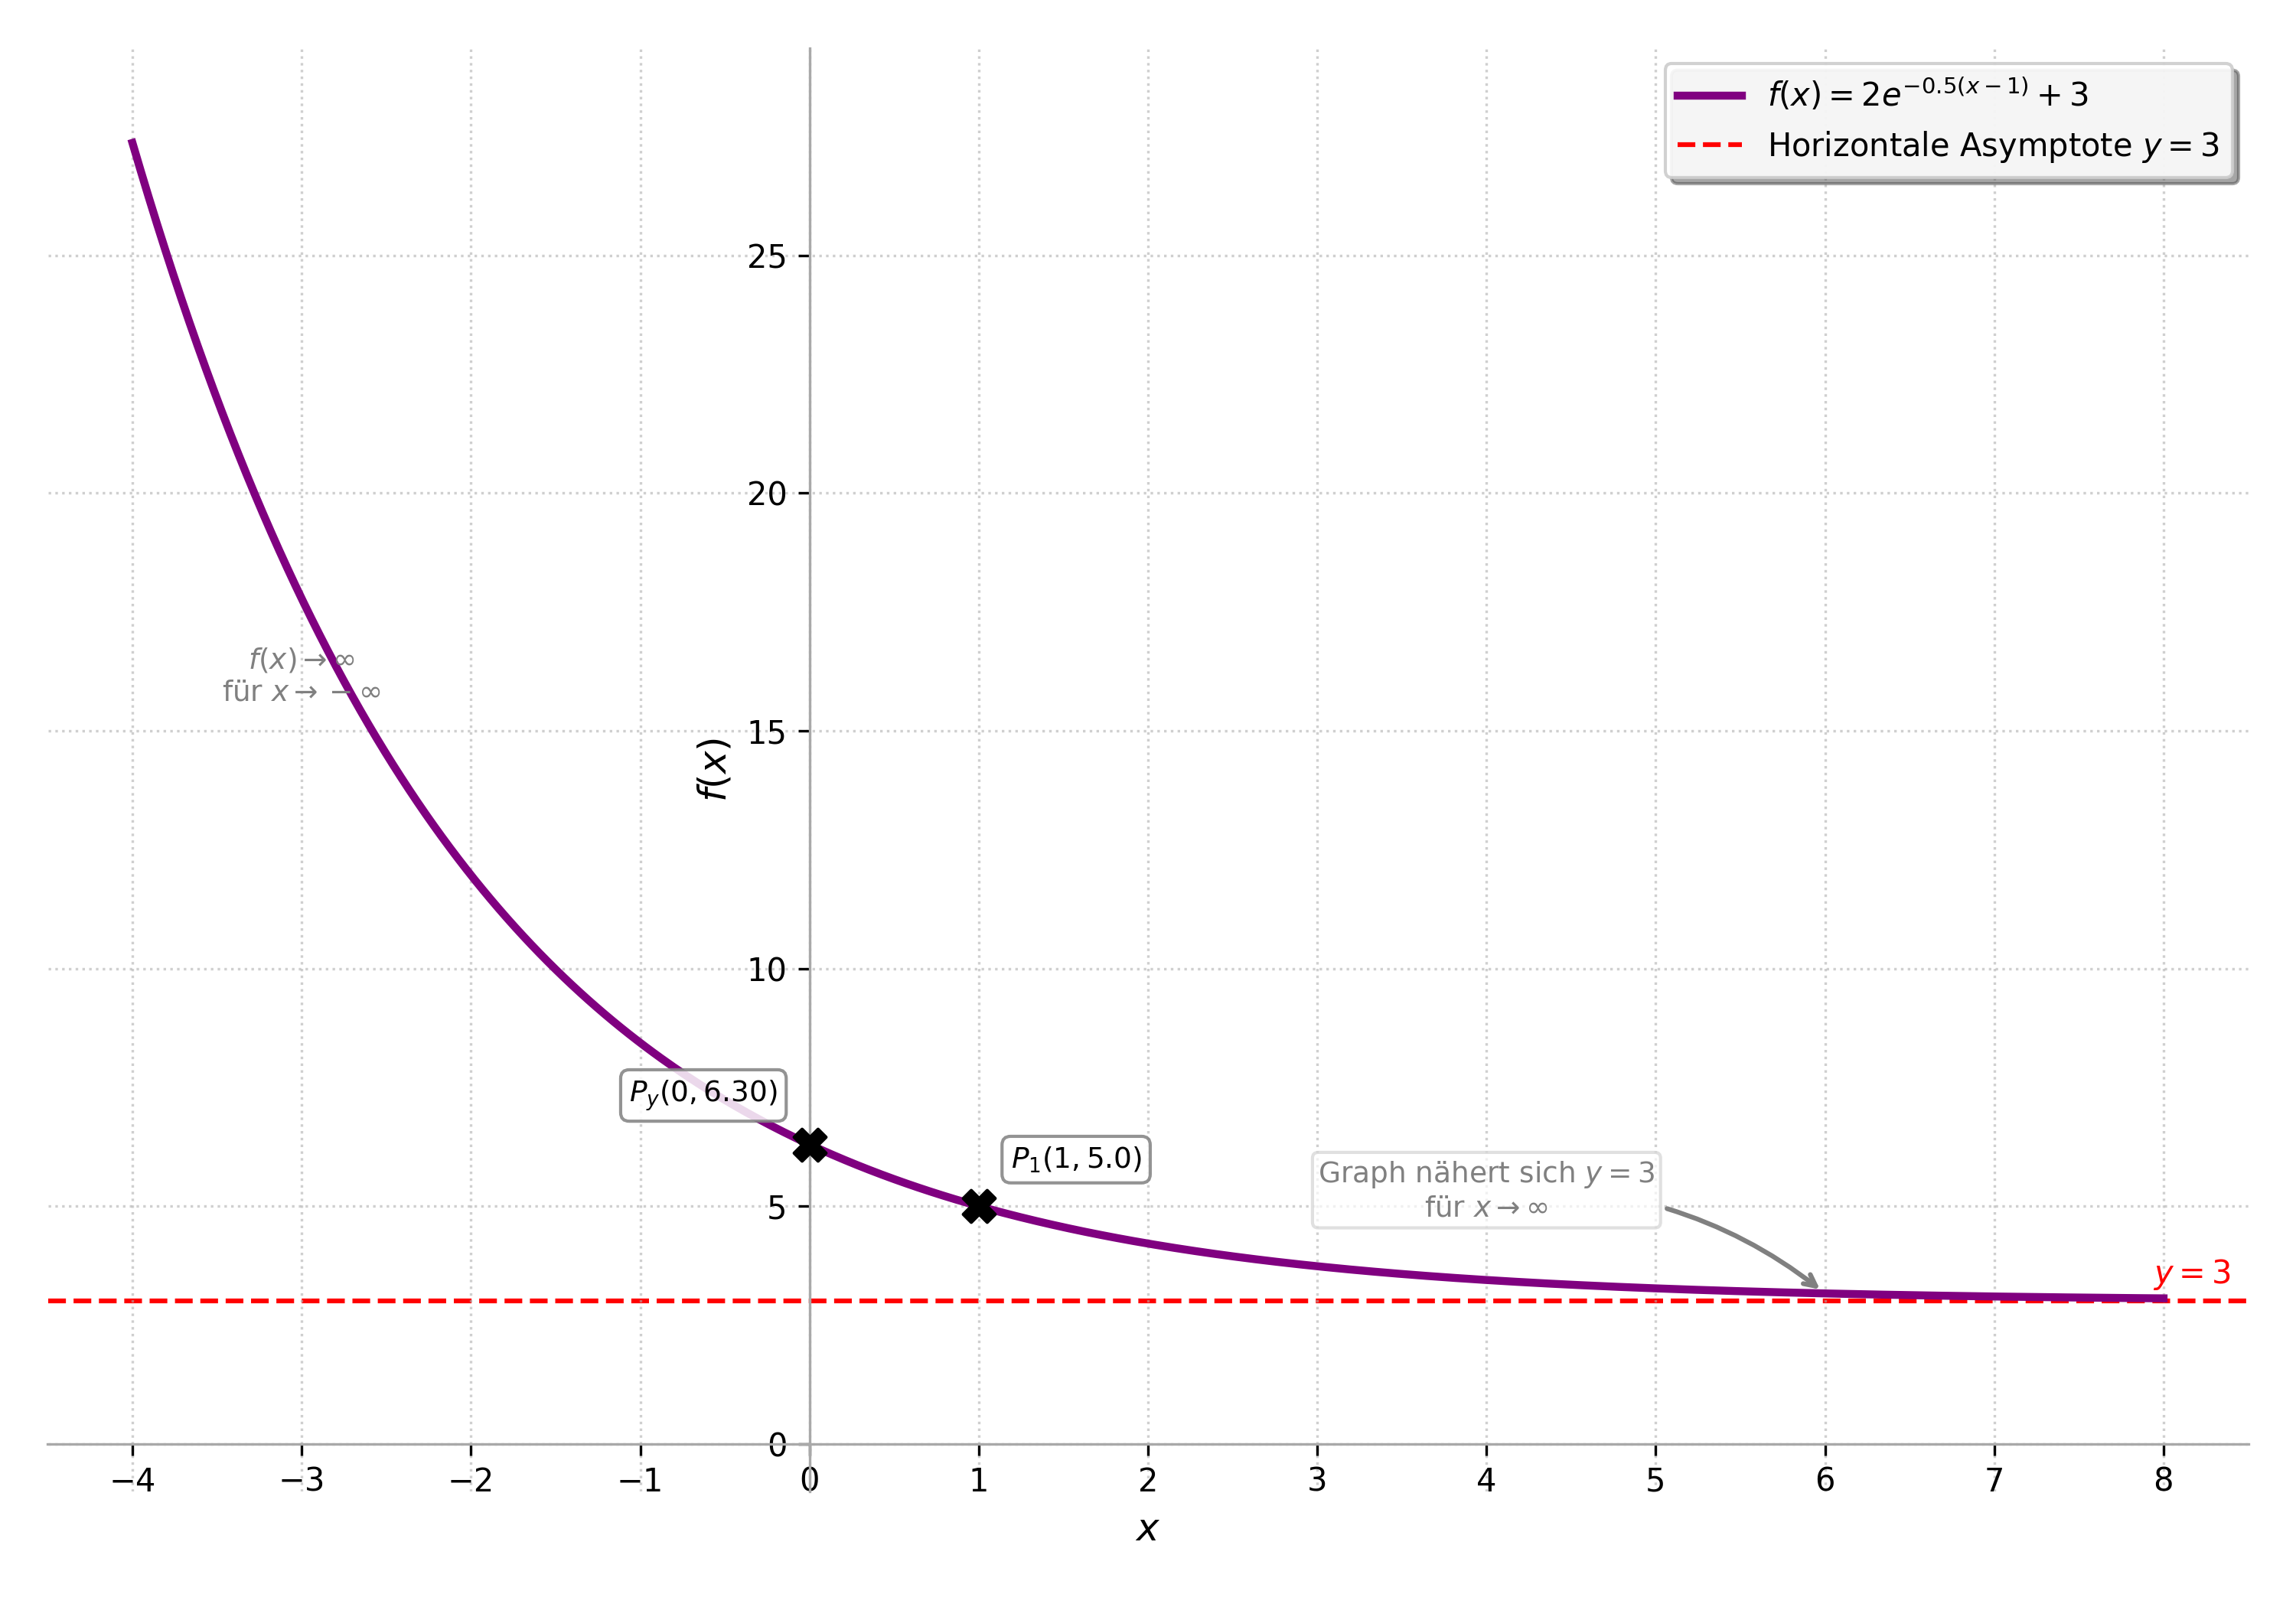
\includegraphics[width=0.8\textwidth]{grafiken/trafo_ex_graph.png}
        % --- Beschreibung der Skizze ---
        % Die Skizze zeigt einen monoton fallenden Graphen.
        % Horizontale Asymptote bei y=3, der sich der Graph für x -> +unendlich von oben nähert.
        % Der Graph verläuft durch den Punkt (1|5). Für x -> -unendlich steigt der Graph ins Unendliche.
        % Der y-Achsenabschnitt liegt bei ca. (0|6.3).
        \captionof{figure}{Graph der Funktion $f(x) = 2e^{-0.5(x-1)} + 3$ mit Asymptote.}
        \label{fig:trafo_ex_graph}
        \end{center}
    \end{itemize}

    \item \textbf{Bilde die erste Ableitung der folgenden Funktionen:}
    Wir verwenden die Kettenregel $(e^{i(x)})' = e^{i(x)} \cdot i'(x)$ und die Faktorregel.
    \begin{itemize}
        \item \textbf{$f_1(x) = 7e^{4x}$} \\
        Innere Funktion $i(x)=4x \Rightarrow i'(x)=4$.
        $f_1'(x) = 7 \cdot e^{4x} \cdot 4 = \mathbf{28e^{4x}}$.

        \item \textbf{$f_2(x) = e^{-x} + 3x$} \\
        Für $e^{-x}$: Innere Funktion $i(x)=-x \Rightarrow i'(x)=-1$.
        $f_2'(x) = e^{-x} \cdot (-1) + 3 = \mathbf{-e^{-x} + 3}$.

        \item \textbf{$f_3(t) = A \cdot e^{-kt}$} ($A, k$ sind positive Konstanten) \\
        Ableitung nach $t$. Innere Funktion $i(t)=-kt \Rightarrow i'(t)=-k$.
        $f_3'(t) = A \cdot e^{-kt} \cdot (-k) = \mathbf{-Ake^{-kt}}$.
    \end{itemize}

    \item \textbf{Bestimme die Menge aller Stammfunktionen:}
    Wir verwenden die Regel $\int e^{ax} \,dx = \frac{1}{a}e^{ax} + C$ (für $a \neq 0$).
    \begin{itemize}
        \item \textbf{$g_1(x) = 10e^{0.2x}$}
        $$ G_1(x) = \int 10e^{0.2x} \,dx = 10 \cdot \frac{1}{0.2} e^{0.2x} + C $$
        Da $\frac{1}{0.2} = \frac{1}{1/5} = 5$:
        $$ G_1(x) = 10 \cdot 5 e^{0.2x} + C = \mathbf{50e^{0.2x} + C} $$

        \item \textbf{$g_2(x) = e^{-3x} - e^{2x}$}
        \begin{align*} G_2(x) &= \int (e^{-3x} - e^{2x}) \,dx \\ &= \int e^{-3x} \,dx - \int e^{2x} \,dx \\ &= \frac{1}{-3}e^{-3x} - \frac{1}{2}e^{2x} + C \\ &= \mathbf{-\frac{1}{3}e^{-3x} - \frac{1}{2}e^{2x} + C} \end{align*}
    \end{itemize}
\end{enumerate}

\end{loesungsumgebung}



\begin{aufgabenumgebung}{Umgang mit allgemeinen Exponentialfunktionen}
\begin{enumerate}
    \item Schreibe die folgenden Funktionen mit der Basis $e$ (d.h. in der Form $a \cdot e^{kx}$):
        \begin{itemize}
            \item $f_1(x) = 3^x$
            \item $f_2(x) = 10 \cdot (0.8)^x$
        \end{itemize}
    \item Bilde die erste Ableitung der folgenden Funktionen:
        \begin{itemize}
            \item $g_1(x) = 4^x + x^4$
            \item $g_2(x) = 7 \cdot (1.5)^x - e^x$
            \item $g_3(t) = P_0 \cdot a^t$ ($P_0$ und $a$ sind positive Konstanten. Dies ist ein typisches Modell für exponentielles Wachstum oder Zerfall, je nachdem ob $a>1$ oder $0<a<1$.)
        \end{itemize}
    \item Bestimme die Menge aller Stammfunktionen:
        \begin{itemize}
            \item $h_1(x) = 5^x$
            \item $h_2(x) = 3 \cdot (0.2)^x + e^{2x}$
        \end{itemize}
    \item \textbf{Vergleich $2^x$ und $e^x$:}
        \begin{itemize}
            \item Skizziere die Graphen von $f(x)=2^x$ und $g(x)=e^x$ in ein gemeinsames Koordinatensystem (z.B. für $x \in [-2, 3]$). Nutze dazu eine Wertetabelle.
            \item Vergleiche die Steigungen der beiden Funktionen an der Stelle $x=0$. Welche Funktion wächst dort schneller?
            \item Berechne $(2^x)'$ und $(e^x)'$.
        \end{itemize}
\end{enumerate}
\end{aufgabenumgebung}

\begin{loesungsumgebung}[loes:allgemeine-exponentialfunktionen]{Umgang mit allgemeinen Exponentialfunktionen}

\begin{enumerate}[label=(\alph*)]
    \item \textbf{Schreibe die folgenden Funktionen mit der Basis $e$ (Form $a \cdot e^{kx}$):}
    \begin{itemize}
        \item \textbf{$f_1(x) = 3^x$} \\
        Wir verwenden die Beziehung $b^x = e^{x \ln b}$.
        $$ f_1(x) = 3^x = e^{\ln(3^x)} = \mathbf{e^{x \ln 3}} $$
        Hier ist der Vorfaktor $a=1$ und $k = \ln 3 \approx 1.0986$.

        \item \textbf{$f_2(x) = 10 \cdot (0.8)^x$} \\
        $$ (0.8)^x = e^{\ln((0.8)^x)} = e^{x \ln 0.8} $$
        Somit:
        $$ f_2(x) = \mathbf{10 \cdot e^{x \ln 0.8}} $$
        Hier ist der Vorfaktor $a=10$ und $k = \ln 0.8 \approx -0.2231$.
    \end{itemize}

    \item \textbf{Bilde die erste Ableitung der folgenden Funktionen:}
    Wir verwenden die Regel $(b^x)' = b^x \ln b$ sowie die Summen- und Faktorregel.
    \begin{itemize}
        \item \textbf{$g_1(x) = 4^x + x^4$}
        $$ g_1'(x) = \frac{d}{dx}(4^x) + \frac{d}{dx}(x^4) = \mathbf{4^x \ln 4 + 4x^3} $$

        \item \textbf{$g_2(x) = 7 \cdot (1.5)^x - e^x$}
        $$ g_2'(x) = 7 \cdot \frac{d}{dx}((1.5)^x) - \frac{d}{dx}(e^x) = \mathbf{7 \cdot (1.5)^x \ln(1.5) - e^x} $$

        \item \textbf{$g_3(t) = P_0 \cdot a^t$} ($P_0$ und $a$ sind positive Konstanten) \\
        Ableitung nach $t$. $P_0$ und $a$ sind Konstanten bezüglich $t$.
        $$ g_3'(t) = P_0 \cdot \frac{d}{dt}(a^t) = \mathbf{P_0 \cdot a^t \ln a} $$
    \end{itemize}

    \item \textbf{Bestimme die Menge aller Stammfunktionen:}
    Wir verwenden die Regel $\int b^x \,dx = \frac{b^x}{\ln b} + C$ (für $b>0, b \neq 1$).
    \begin{itemize}
        \item \textbf{$h_1(x) = 5^x$}
        $$ H_1(x) = \int 5^x \,dx = \mathbf{\frac{5^x}{\ln 5} + C} $$

        \item \textbf{$h_2(x) = 3 \cdot (0.2)^x + e^{2x}$}
        \begin{align*} H_2(x) &= \int (3 \cdot (0.2)^x + e^{2x}) \,dx \\ &= 3 \int (0.2)^x \,dx + \int e^{2x} \,dx \\ &= 3 \cdot \frac{(0.2)^x}{\ln 0.2} + \frac{1}{2}e^{2x} + C \\ &= \mathbf{\frac{3 \cdot (0.2)^x}{\ln 0.2} + \frac{1}{2}e^{2x} + C} \end{align*}
        (Beachte: $\ln 0.2 = \ln(1/5) = -\ln 5$ ist negativ.)
    \end{itemize}

    \item \textbf{Vergleich $2^x$ und $e^x$:}
    \begin{itemize}
        \item \textbf{Skizziere die Graphen von $f(x)=2^x$ und $g(x)=e^x$ in ein gemeinsames Koordinatensystem (z.B. für $x \in [-2, 3]$). Nutze dazu eine Wertetabelle.} \\
        \textbf{Wertetabelle:}
        \begin{center}
        \begin{tabular}{c|c|c}
        $x$ & $f(x)=2^x$ & $g(x)=e^x$ (ca.) \\
        \hline
        -2 & $2^{-2} = 0.25$ & $e^{-2} \approx 0.135$ \\
        -1 & $2^{-1} = 0.5$ & $e^{-1} \approx 0.368$ \\
        0 & $2^0 = 1$ & $e^0 = 1$ \\
        1 & $2^1 = 2$ & $e^1 \approx 2.718$ \\
        2 & $2^2 = 4$ & $e^2 \approx 7.389$ \\
        3 & $2^3 = 8$ & $e^3 \approx 20.086$ \\
        \end{tabular}
        \end{center}
        \begin{center}
        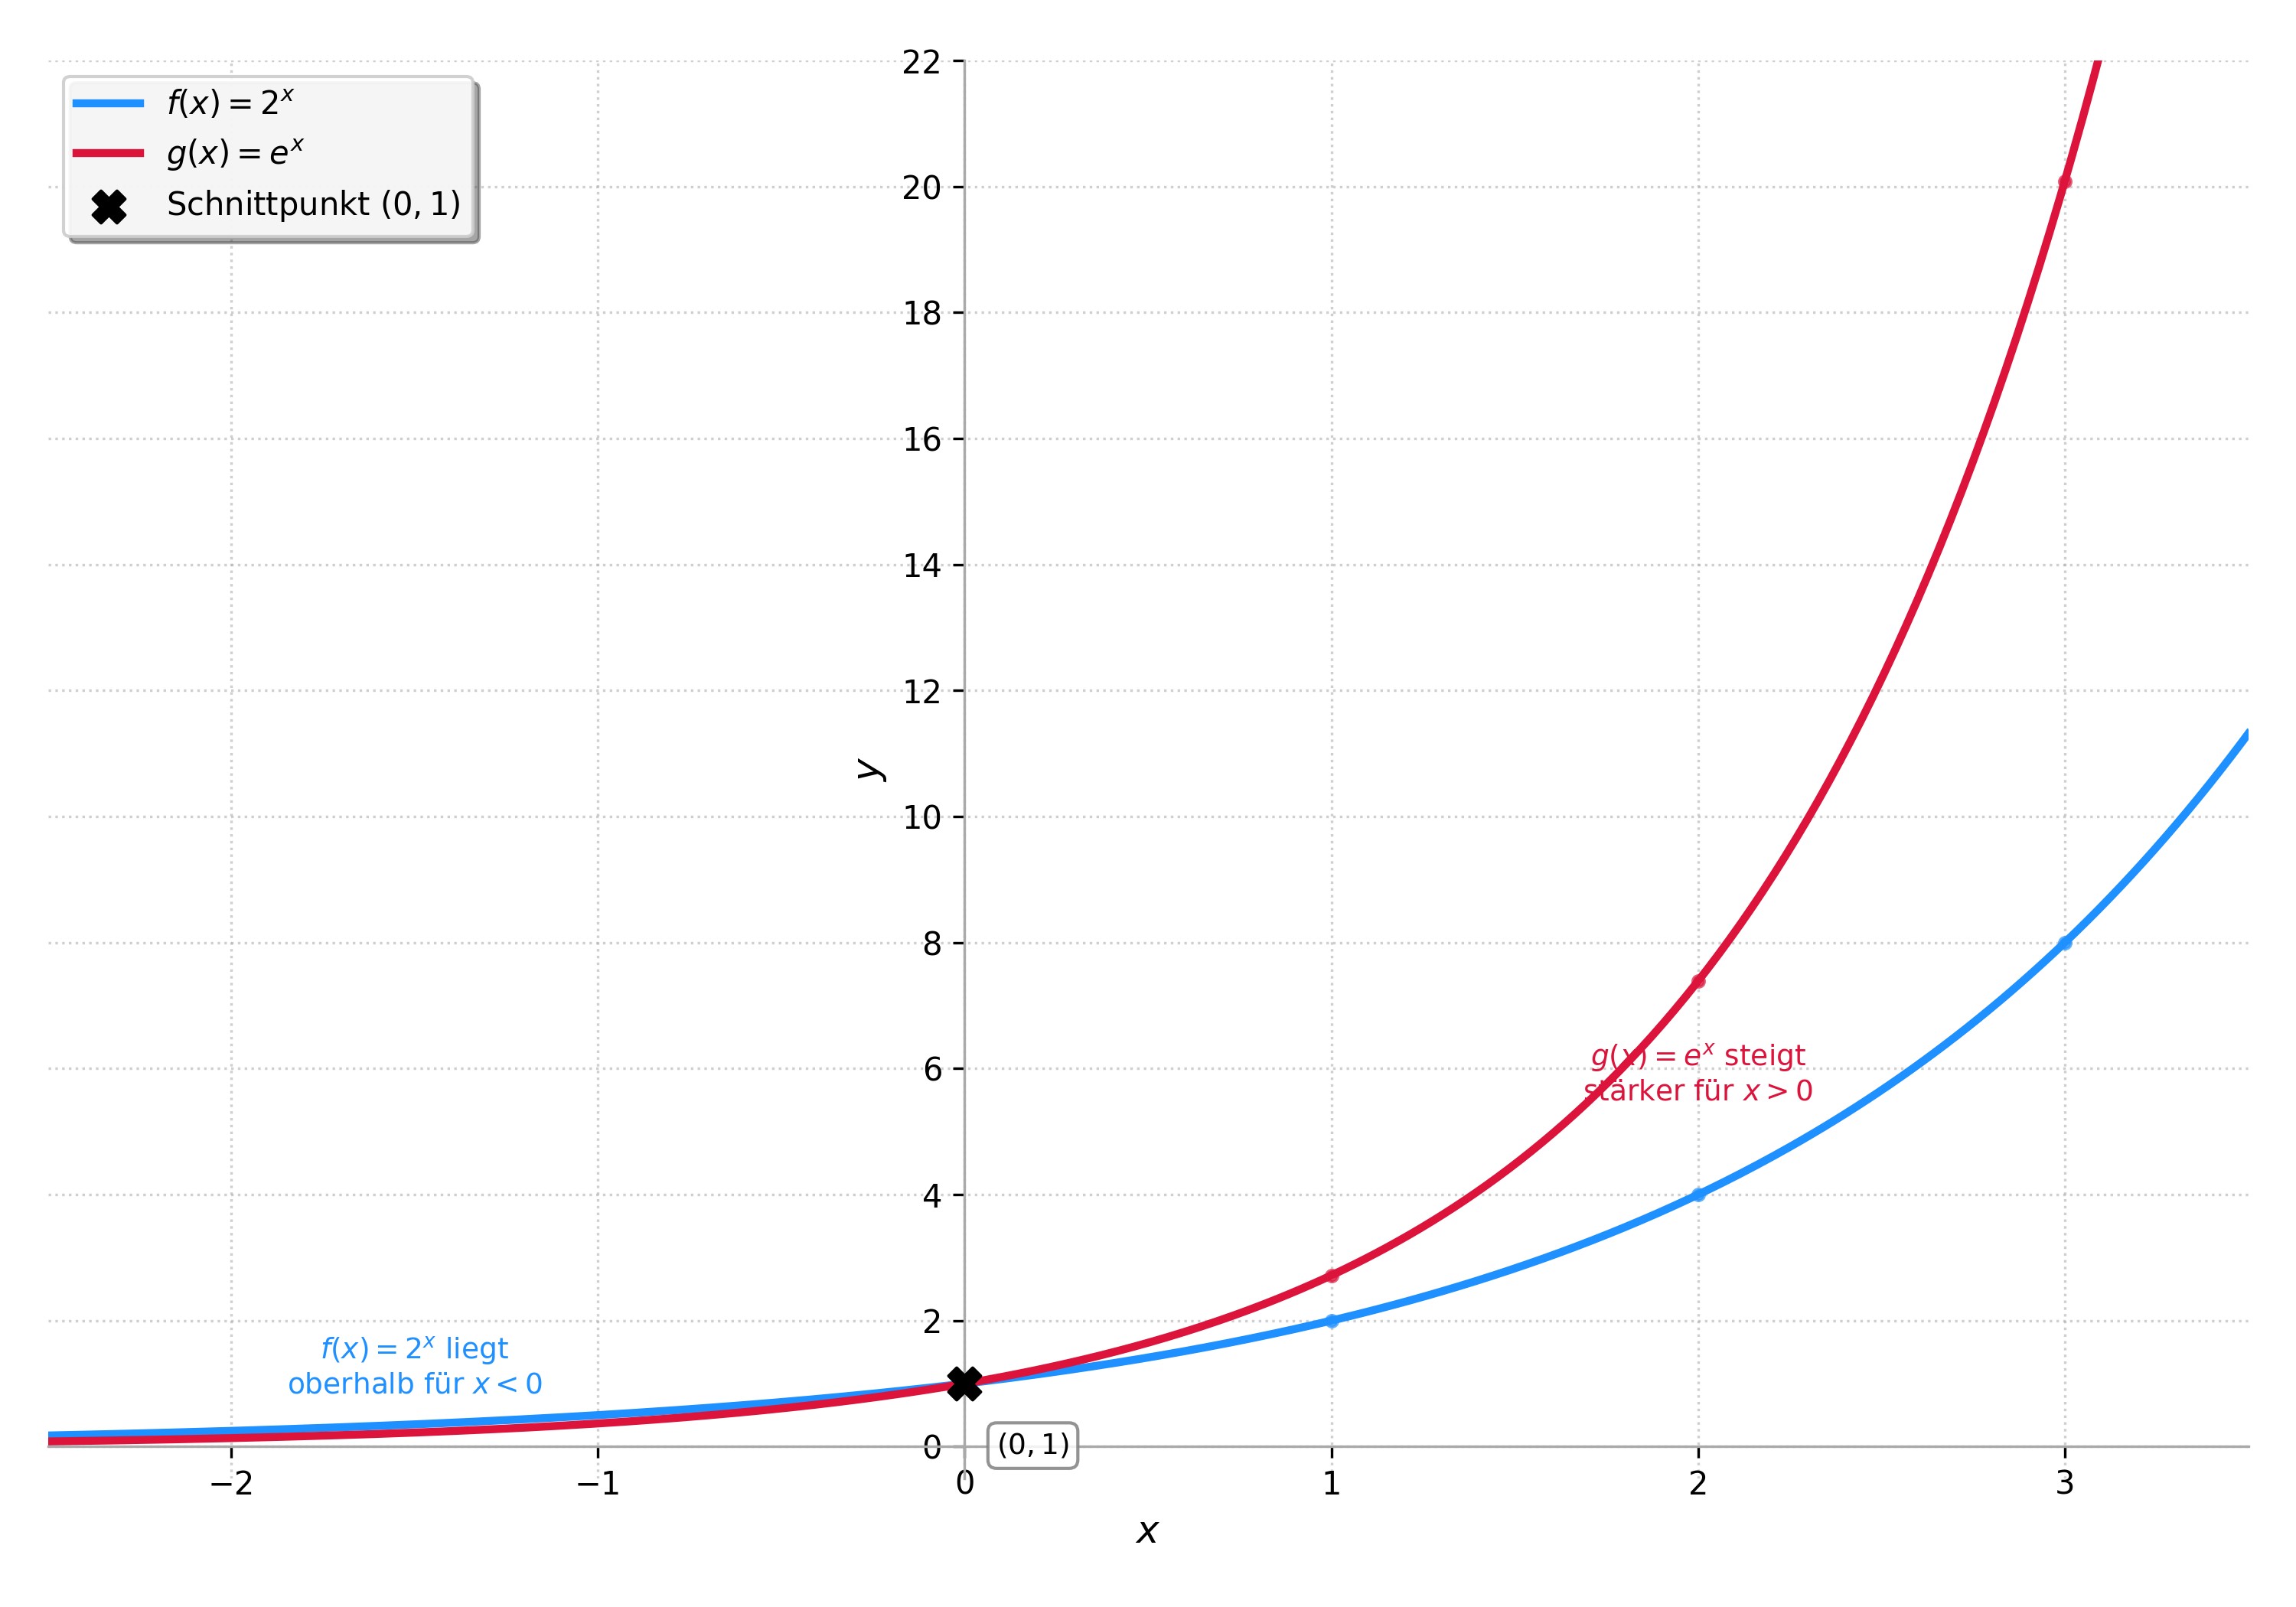
\includegraphics[width=0.8\textwidth]{grafiken/vergleich_2x_ex.png}
        % --- Beschreibung der Skizze ---
        % Die Skizze zeigt ein Koordinatensystem mit x-Achse von -2 bis 3 und y-Achse von 0 bis ca. 21.
        % Zwei Graphen sind eingezeichnet:
        % 1. f(x)=2^x: Startet flach für negative x, geht durch (0|1), (1|2), (2|4), (3|8).
        % 2. g(x)=e^x: Startet noch flacher als 2^x für negative x, geht ebenfalls durch (0|1), dann (1|e approx 2.72), (2|e^2 approx 7.39), (3|e^3 approx 20.09).
        % Beide Graphen sind streng monoton steigend und schneiden sich bei (0|1).
        % Für x > 0 liegt der Graph von e^x oberhalb des Graphen von 2^x und steigt steiler an.
        % Für x < 0 liegt der Graph von e^x unterhalb des Graphen von 2^x und nähert sich schneller der x-Achse.
        \captionof{figure}{Vergleich der Graphen von $f(x)=2^x$ und $g(x)=e^x$.}
        \label{fig:vergleich_2x_ex}
        \end{center}

        \item \textbf{Vergleiche die Steigungen der beiden Funktionen an der Stelle $x=0$. Welche Funktion wächst dort schneller?}
        Die Steigung ist gegeben durch die erste Ableitung:
        Für $f(x)=2^x$: $f'(x) = 2^x \ln 2$.
        An der Stelle $x=0$: $f'(0) = 2^0 \ln 2 = 1 \cdot \ln 2 = \ln 2 \approx 0.693$.
        Für $g(x)=e^x$: $g'(x) = e^x$.
        An der Stelle $x=0$: $g'(0) = e^0 = 1$.
        Da $1 > \ln 2 \approx 0.693$, ist die Steigung von $g(x)=e^x$ an der Stelle $x=0$ größer als die von $f(x)=2^x$.
        Die Funktion $\mathbf{g(x)=e^x}$ wächst an der Stelle $x=0$ schneller.

        \item \textbf{Berechne $(2^x)'$ und $(e^x)'$.}
        $(2^x)' = \mathbf{2^x \ln 2}$.
        $(e^x)' = \mathbf{e^x}$.
    \end{itemize}
\end{enumerate}

\end{loesungsumgebung}


\begin{aufgabenumgebung}{Produktregel mit $e^x$ üben}
Bilde die erste Ableitung der folgenden Funktionen und vereinfache so weit wie möglich:
\begin{enumerate}
    \item $f_1(x) = (3x-1)e^x$
    \item $f_2(x) = (x^2+2x-5)e^x$
    \item $f_3(t) = t \cdot e^{2t}$ (Hier ist die Kettenregel für $e^{2t}$ zusätzlich nötig!)
\end{enumerate}
\end{aufgabenumgebung}

\begin{loesungsumgebung}[loes:produktregel-ex-ueben]{Produktregel mit $e^x$ üben}
Wir wenden die Produktregel $f'(x) = u'(x)v(x) + u(x)v'(x)$ an. Bei Bedarf wird zusätzlich die Kettenregel für die Ableitung der e-Funktion genutzt: $(e^{i(x)})' = e^{i(x)} \cdot i'(x)$.

\begin{enumerate}[label=(\alph*)]
    \item \textbf{Funktion $f_1(x) = (3x-1)e^x$} \\
    Sei $u(x) = 3x-1 \Rightarrow u'(x) = 3$. \\
    Sei $v(x) = e^x \Rightarrow v'(x) = e^x$.
    \begin{align*}
    f_1'(x) &= u'(x)v(x) + u(x)v'(x) \\
            &= 3 \cdot e^x + (3x-1) \cdot e^x \\
            &= e^x (3 + (3x-1)) \quad (\text{Ausklammern von } e^x) \\
            &= e^x (3 + 3x - 1) \\
            &= \mathbf{e^x (3x + 2)}
    \end{align*}

    \item \textbf{Funktion $f_2(x) = (x^2+2x-5)e^x$} \\
    Sei $u(x) = x^2+2x-5 \Rightarrow u'(x) = 2x+2$. \\
    Sei $v(x) = e^x \Rightarrow v'(x) = e^x$.
    \begin{align*}
    f_2'(x) &= u'(x)v(x) + u(x)v'(x) \\
            &= (2x+2)e^x + (x^2+2x-5)e^x \\
            &= e^x [(2x+2) + (x^2+2x-5)] \quad (\text{Ausklammern von } e^x) \\
            &= e^x (x^2 + 2x + 2x + 2 - 5) \\
            &= \mathbf{e^x (x^2 + 4x - 3)}
    \end{align*}

    \item \textbf{Funktion $f_3(t) = t \cdot e^{2t}$} \\
    Hier leiten wir nach $t$ ab.
    Sei $u(t) = t \Rightarrow u'(t) = 1$. \\
    Sei $v(t) = e^{2t}$. Für $v'(t)$ benötigen wir die Kettenregel:
    Die innere Funktion ist $i(t)=2t \Rightarrow i'(t)=2$. Die äußere Funktion ist $a_v(w)=e^w \Rightarrow a_v'(w)=e^w$.
    $v'(t) = e^{2t} \cdot 2 = 2e^{2t}$.
    \begin{align*}
    f_3'(t) &= u'(t)v(t) + u(t)v'(t) \\
             &= 1 \cdot e^{2t} + t \cdot (2e^{2t}) \\
             &= e^{2t} + 2te^{2t} \\
             &= \mathbf{e^{2t} (1 + 2t)} \quad (\text{Ausklammern von } e^{2t})
    \end{align*}
\end{enumerate}

\end{loesungsumgebung}

\begin{aufgabenumgebung}{Quotientenregel mit $e^x$ üben}
Bilde die erste Ableitung der folgenden Funktionen und vereinfache so weit wie möglich. Gib auch den Definitionsbereich an.
\begin{enumerate}
    \item $f_1(x) = \frac{x+2}{e^x}$
    \item $f_2(x) = \frac{e^{3x}}{2x-1}$ (Kettenregel für $e^{3x}$ nötig!)
\end{enumerate}
\end{aufgabenumgebung}

\begin{loesungsumgebung}[loes:quotientenregel-ex-ueben]{Quotientenregel mit $e^x$ üben}
Wir bestimmen die erste Ableitung der gegebenen Funktionen mithilfe der Quotientenregel $f'(x) = \frac{u'(x)v(x) - u(x)v'(x)}{[v(x)]^2}$ und geben den Definitionsbereich an.

\begin{enumerate}[label=(\alph*)]
    \item \textbf{Funktion $f_1(x) = \frac{x+2}{e^x}$}
    \begin{itemize}
        \item \textbf{Definitionsbereich:} Der Nenner $e^x$ ist für alle reellen Zahlen $x$ definiert und stets $e^x > 0$, also nie Null.
        Somit ist $D_{f_1} = \mathbb{R}$.
        \item \textbf{Ableitung mit Quotientenregel:} \\
        Sei $u(x) = x+2 \Rightarrow u'(x) = 1$. \\
        Sei $v(x) = e^x \Rightarrow v'(x) = e^x$.
        \begin{align*}
        f_1'(x) &= \frac{u'(x)v(x) - u(x)v'(x)}{[v(x)]^2} \\
                &= \frac{1 \cdot e^x - (x+2) \cdot e^x}{(e^x)^2} \\
                &= \frac{e^x (1 - (x+2))}{(e^x)^2} \quad (\text{Ausklammern von } e^x \text{ im Zähler}) \\
                &= \frac{1 - x - 2}{e^x} \quad (\text{Kürzen von } e^x) \\
                &= \mathbf{\frac{-x - 1}{e^x}} \quad \text{oder} \quad \mathbf{-\frac{x+1}{e^x}}
        \end{align*}
        \textit{Alternative Schreibweise:} $f_1'(x) = -(x+1)e^{-x}$.
    \end{itemize}

    \item \textbf{Funktion $f_2(x) = \frac{e^{3x}}{2x-1}$}
    \begin{itemize}
        \item \textbf{Definitionsbereich:} Der Nenner $2x-1$ darf nicht Null sein: $2x-1 \neq 0 \Rightarrow 2x \neq 1 \Rightarrow x \neq \frac{1}{2}$.
        Somit ist $D_{f_2} = \mathbb{R} \setminus \{\frac{1}{2}\}$.
        \item \textbf{Ableitung mit Quotientenregel:} \\
        Sei $u(x) = e^{3x}$. Für $u'(x)$ benötigen wir die Kettenregel:
        Innere Funktion $i(x)=3x \Rightarrow i'(x)=3$. Äußere Funktion $a_u(w)=e^w \Rightarrow a_u'(w)=e^w$.
        $u'(x) = e^{3x} \cdot 3 = 3e^{3x}$. \\
        Sei $v(x) = 2x-1 \Rightarrow v'(x) = 2$.
        \begin{align*}
        f_2'(x) &= \frac{u'(x)v(x) - u(x)v'(x)}{[v(x)]^2} \\
                &= \frac{(3e^{3x})(2x-1) - (e^{3x})(2)}{(2x-1)^2} \\
                &= \frac{e^{3x} [3(2x-1) - 2]}{(2x-1)^2} \quad (\text{Ausklammern von } e^{3x} \text{ im Zähler}) \\
                &= \frac{e^{3x} (6x - 3 - 2)}{(2x-1)^2} \\
                &= \mathbf{\frac{e^{3x}(6x-5)}{(2x-1)^2}}
        \end{align*}
    \end{itemize}
\end{enumerate}

\end{loesungsumgebung}

\begin{aufgabenumgebung}{Kettenregel mit $e^x$ weiter üben}
Bilde die erste Ableitung:
\begin{enumerate}
    \item $f_1(x) = e^{-x^2}$
    \item $f_2(x) = 5e^{2x^3-4x+1}$
    \item $f_3(x) = (e^x+1)^3$ (Hier ist $e^x+1$ die innere Funktion und $(\dots)^3$ die äußere.)
\end{enumerate}
\end{aufgabenumgebung}

\begin{loesungsumgebung}[loes:kettenregel-ex-weiter-ueben]{Kettenregel mit $e^x$ weiter üben}
Wir bilden die erste Ableitung der gegebenen Funktionen mithilfe der Kettenregel.

\begin{enumerate}[label=(\alph*)]
    \item \textbf{Funktion $f_1(x) = e^{-x^2}$}
    \begin{itemize}
        \item Äußere Funktion: $a(u) = e^u \Rightarrow a'(u) = e^u$.
        \item Innere Funktion: $i(x) = -x^2 \Rightarrow i'(x) = -2x$.
    \end{itemize}
    Anwendung der Kettenregel:
    \begin{align*}
    f_1'(x) &= a'(i(x)) \cdot i'(x) \\
            &= e^{-x^2} \cdot (-2x) \\
            &= \mathbf{-2xe^{-x^2}}
    \end{align*}

    \item \textbf{Funktion $f_2(x) = 5e^{2x^3-4x+1}$}
    \begin{itemize}
        \item Äußere Funktion: $a(u) = 5e^u \Rightarrow a'(u) = 5e^u$.
        \item Innere Funktion: $i(x) = 2x^3-4x+1 \Rightarrow i'(x) = 6x^2-4$.
    \end{itemize}
    Anwendung der Kettenregel:
    \begin{align*}
    f_2'(x) &= a'(i(x)) \cdot i'(x) \\
            &= 5e^{2x^3-4x+1} \cdot (6x^2-4) \\
            &= \mathbf{5(6x^2-4)e^{2x^3-4x+1}} \quad \text{oder} \quad \mathbf{(30x^2-20)e^{2x^3-4x+1}}
    \end{align*}

    \item \textbf{Funktion $f_3(x) = (e^x+1)^3$} \\
    Hier ist $e^x+1$ die innere Funktion und $(\dots)^3$ die äußere.
    \begin{itemize}
        \item Äußere Funktion: $a(u) = u^3 \Rightarrow a'(u) = 3u^2$.
        \item Innere Funktion: $i(x) = e^x+1 \Rightarrow i'(x) = e^x$.
    \end{itemize}
    Anwendung der Kettenregel:
    \begin{align*}
    f_3'(x) &= a'(i(x)) \cdot i'(x) \\
            &= 3(e^x+1)^2 \cdot e^x \\
            &= \mathbf{3e^x(e^x+1)^2}
    \end{align*}
\end{enumerate}

\end{loesungsumgebung}


\begin{aufgabenumgebung}{Kombinierte Anwendung: Produkt- und Kettenregel bei e-Funktionen}
Bilde die erste Ableitung der folgenden Funktionen. Vereinfache das Ergebnis so weit wie möglich, indem du z.B. gemeinsame Faktoren (insbesondere den $e$-Term) ausklammerst.
\begin{enumerate}
    \item $f(x) = (2x^2 - 3x + 1) \cdot e^{x^2 - 4}$
    \item $g(x) = (x+1)^2 \cdot e^{-2x}$
\end{enumerate}
\end{aufgabenumgebung}

\begin{loesungsumgebung}[loes:produkt-kette-e-funktionen]{Kombinierte Anwendung: Produkt- und Kettenregel bei e-Funktionen}
Wir bilden die erste Ableitung der gegebenen Funktionen und vereinfachen die Ergebnisse.

\begin{enumerate}[label=(\alph*)]
    \item \textbf{Funktion $f(x) = (2x^2 - 3x + 1) \cdot e^{x^2 - 4}$} \\
    Diese Funktion ist ein Produkt $f(x) = u(x) \cdot v(x)$. Wir wenden die Produktregel an: $f'(x) = u'(x)v(x) + u(x)v'(x)$.
    \begin{itemize}
        \item Sei $u(x) = 2x^2 - 3x + 1 \Rightarrow u'(x) = 4x - 3$.
        \item Sei $v(x) = e^{x^2 - 4}$. Für $v'(x)$ benötigen wir die Kettenregel:
        Die äußere Funktion ist $a_v(w) = e^w \Rightarrow a_v'(w) = e^w$.
        Die innere Funktion ist $i_v(x) = x^2 - 4 \Rightarrow i_v'(x) = 2x$.
        Somit ist $v'(x) = a_v'(i_v(x)) \cdot i_v'(x) = e^{x^2 - 4} \cdot 2x = 2xe^{x^2 - 4}$.
    \end{itemize}
    Anwendung der Produktregel:
    \begin{align*}
    f'(x) &= (4x - 3) \cdot e^{x^2 - 4} + (2x^2 - 3x + 1) \cdot (2xe^{x^2 - 4}) \\
          &= e^{x^2 - 4} \left[ (4x - 3) + (2x^2 - 3x + 1)(2x) \right] \quad (\text{Ausklammern von } e^{x^2-4}) \\
          &= e^{x^2 - 4} [4x - 3 + 4x^3 - 6x^2 + 2x] \\
          &= e^{x^2 - 4} (4x^3 - 6x^2 + 6x - 3) \\
          &= \mathbf{(4x^3 - 6x^2 + 6x - 3)e^{x^2 - 4}}
    \end{align*}

    \item \textbf{Funktion $g(x) = (x+1)^2 \cdot e^{-2x}$} \\
    Dies ist ein Produkt $g(x) = u(x) \cdot v(x)$.
    \begin{itemize}
        \item Sei $u(x) = (x+1)^2$. Für $u'(x)$ mit Kettenregel:
        Äußere Funktion $a_u(w) = w^2 \Rightarrow a_u'(w) = 2w$.
        Innere Funktion $i_u(x) = x+1 \Rightarrow i_u'(x) = 1$.
        $u'(x) = 2(x+1) \cdot 1 = 2(x+1)$.
        \item Sei $v(x) = e^{-2x}$. Für $v'(x)$ mit Kettenregel:
        Äußere Funktion $a_v(w) = e^w \Rightarrow a_v'(w) = e^w$.
        Innere Funktion $i_v(x) = -2x \Rightarrow i_v'(x) = -2$.
        $v'(x) = e^{-2x} \cdot (-2) = -2e^{-2x}$.
    \end{itemize}
    Anwendung der Produktregel:
    \begin{align*}
    g'(x) &= u'(x)v(x) + u(x)v'(x) \\
          &= 2(x+1)e^{-2x} + (x+1)^2(-2e^{-2x}) \\
          &= 2(x+1)e^{-2x} [1 - (x+1)] \quad (\text{Ausklammern von } 2(x+1)e^{-2x}) \\
          &= 2(x+1)e^{-2x} [1 - x - 1] \\
          &= 2(x+1)e^{-2x} [-x] \\
          &= \mathbf{-2x(x+1)e^{-2x}}
    \end{align*}

    \textbf{Alternative Lösung für $g(x)$ durch Ausmultiplizieren des Binoms $(x+1)^2$ zuerst:} \\
    $g(x) = (x^2+2x+1) \cdot e^{-2x}$.
    Sei nun $u(x) = x^2+2x+1 \Rightarrow u'(x) = 2x+2$.
    Sei $v(x) = e^{-2x} \Rightarrow v'(x) = -2e^{-2x}$ (wie oben).
    Anwendung der Produktregel:
    \begin{align*}
    g'(x) &= (2x+2)e^{-2x} + (x^2+2x+1)(-2e^{-2x}) \\
          &= e^{-2x} [(2x+2) - 2(x^2+2x+1)] \quad (\text{Ausklammern von } e^{-2x}) \\
          &= e^{-2x} [2x+2 - 2x^2-4x-2] \\
          &= e^{-2x} [-2x^2 - 2x] \\
          &= e^{-2x} [-2x(x+1)] \\
          &= \mathbf{-2x(x+1)e^{-2x}}
    \end{align*}
    Beide Lösungswege führen zum selben Ergebnis.
\end{enumerate}

\end{loesungsumgebung}


\begin{aufgabenumgebung}{Kurvendiskussionen mit Exponentialfunktionen}
Führe eine vollständige Kurvendiskussion für die folgenden Funktionen durch.
\begin{enumerate}
    \item $f(x) = x e^{-x}$
    \item $g(x) = (x^2-2)e^x$
    \item \textbf{Für Experten:} $h(x) = e^{x^2-2x}$. (Hier wird die Kettenregel komplexer, aber die Struktur der Kurvendiskussion bleibt gleich.)
\end{enumerate}
\end{aufgabenumgebung}



\begin{loesungsumgebung}[loes:kurvendiskussion-ex-funktionen]{Kurvendiskussionen mit Exponentialfunktionen}

\begin{enumerate}[label=(\alph*)]
    \item \textbf{Funktion $f(x) = x e^{-x}$}

    \subsubsection*{1. Definitionsbereich}
    Die Funktion $f(x)$ ist als Produkt einer linearen Funktion ($x$) und einer Exponentialfunktion ($e^{-x}$) für alle reellen Zahlen definiert.
    $D_f = \mathbb{R}$.

    \subsubsection*{2. Symmetrie}
    $f(-x) = (-x)e^{-(-x)} = -xe^x$.
    Da $f(-x) \neq f(x)$ und $f(-x) \neq -f(x)$ (z.B. $f(1)=e^{-1}$, $f(-1)=-e$, $-f(1)=-e^{-1}$), liegt keine einfache Achsen- oder Punktsymmetrie zum Ursprung vor.

    \subsubsection*{3. Verhalten im Unendlichen}
    \begin{itemize}
        \item Für $x \to \infty$: $\lim_{x \to \infty} x e^{-x} = \lim_{x \to \infty} \frac{x}{e^x}$. Da $e^x$ schneller wächst als $x$ (Regel von L'Hôpital anwendbar: $\lim \frac{1}{e^x} = 0$), gilt $\lim_{x \to \infty} f(x) = 0$.
        Somit ist $y=0$ eine horizontale Asymptote für $x \to \infty$.
        \item Für $x \to -\infty$: Sei $u = -x$. Dann $u \to \infty$.
        $\lim_{x \to -\infty} x e^{-x} = \lim_{u \to \infty} (-u)e^u = -\infty \cdot \infty = -\infty$.
    \end{itemize}

    \subsubsection*{4. Achsenschnittpunkte}
    \begin{itemize}
        \item y-Achsenabschnitt (für $x=0$): $f(0) = 0 \cdot e^0 = 0 \cdot 1 = 0$. Punkt $P_y(0|0)$.
        \item Nullstellen (für $f(x)=0$): $xe^{-x} = 0$. Da $e^{-x} > 0$ für alle $x$, muss $x=0$ sein.
        Die einzige Nullstelle ist $x_N=0$.
    \end{itemize}

    \subsubsection*{5. Erste Ableitung $f'(x)$}
    Mit der Produktregel ($u=x, u'=1; v=e^{-x}, v'=-e^{-x}$):
    $f'(x) = 1 \cdot e^{-x} + x \cdot (-e^{-x}) = e^{-x} - xe^{-x} = \mathbf{e^{-x}(1-x)}$.

    \subsubsection*{6. Extrempunkte}
    Notwendige Bedingung: $f'(x)=0$.
    $e^{-x}(1-x) = 0$. Da $e^{-x} \neq 0$, muss $1-x=0 \Rightarrow x=1$.
    Potenzielle Extremstelle $x_E=1$. $f(1) = 1 \cdot e^{-1} = \frac{1}{e}$.
    Hinreichende Bedingung (mit $f''(x)$, siehe unten): $f''(1) = e^{-1}(1-2) = -e^{-1} < 0$.
    Also liegt ein lokaler Hochpunkt bei $H(1 | \frac{1}{e} \approx 0.368)$ vor.

    \subsubsection*{7. Monotonieverhalten}
    Das Vorzeichen von $f'(x) = e^{-x}(1-x)$ hängt vom Faktor $(1-x)$ ab, da $e^{-x}>0$.
    \begin{itemize}
        \item Für $x < 1$: $1-x > 0 \Rightarrow f'(x) > 0 \Rightarrow f(x)$ ist streng monoton steigend.
        \item Für $x > 1$: $1-x < 0 \Rightarrow f'(x) < 0 \Rightarrow f(x)$ ist streng monoton fallend.
    \end{itemize}

    \subsubsection*{8. Zweite Ableitung $f''(x)$}
    Mit der Produktregel für $f'(x)=e^{-x}(1-x)$ ($u=e^{-x}, u'=-e^{-x}; v=1-x, v'=-1$):
    $f''(x) = (-e^{-x})(1-x) + e^{-x}(-1) = -e^{-x} + xe^{-x} - e^{-x} = xe^{-x} - 2e^{-x} = \mathbf{e^{-x}(x-2)}$.

    \subsubsection*{9. Wendepunkte}
    Notwendige Bedingung: $f''(x)=0$.
    $e^{-x}(x-2) = 0$. Da $e^{-x} \neq 0$, muss $x-2=0 \Rightarrow x=2$.
    Potenzielle Wendestelle $x_W=2$. $f(2) = 2e^{-2} = \frac{2}{e^2}$.
    Hinreichende Bedingung (mit $f'''(x)$):
    $f'''(x) = \frac{d}{dx}(e^{-x}(x-2)) = (-e^{-x})(x-2) + e^{-x}(1) = e^{-x}(-x+2+1) = e^{-x}(3-x)$.
    $f'''(2) = e^{-2}(3-2) = e^{-2} \neq 0$.
    Also liegt ein Wendepunkt bei $W(2 | \frac{2}{e^2} \approx 0.271)$ vor.

    \subsubsection*{10. Krümmungsverhalten}
    Das Vorzeichen von $f''(x) = e^{-x}(x-2)$ hängt von $(x-2)$ ab.
    \begin{itemize}
        \item Für $x < 2$: $x-2 < 0 \Rightarrow f''(x) < 0 \Rightarrow f(x)$ ist rechtsgekrümmt (konkav).
        \item Für $x > 2$: $x-2 > 0 \Rightarrow f''(x) > 0 \Rightarrow f(x)$ ist linksgekrümmt (konvex).
    \end{itemize}

    \subsubsection*{11. Wertebereich}
    $W_f = (-\infty, \frac{1}{e}]$.

    \item \textbf{Funktion $g(x) = (x^2-2)e^x$}

    \subsubsection*{1. Definitionsbereich}
    $D_g = \mathbb{R}$.

    \subsubsection*{2. Symmetrie}
    $g(-x) = ((-x)^2-2)e^{-x} = (x^2-2)e^{-x}$. Keine einfache Symmetrie.

    \subsubsection*{3. Verhalten im Unendlichen}
    \begin{itemize}
        \item Für $x \to \infty$: $\lim_{x \to \infty} (x^2-2)e^x = \infty \cdot \infty = \infty$.
        \item Für $x \to -\infty$: $\lim_{x \to -\infty} (x^2-2)e^x = \lim_{x \to -\infty} \frac{x^2-2}{e^{-x}}$. Mit L'Hôpital (zweimal):
        $\lim_{x \to -\infty} \frac{2x}{-e^{-x}} = \lim_{x \to -\infty} \frac{2}{e^{-x}} = 0$.
        Somit ist $y=0$ eine horizontale Asymptote für $x \to -\infty$.
    \end{itemize}

    \subsubsection*{4. Achsenschnittpunkte}
    \begin{itemize}
        \item y-Achsenabschnitt ($x=0$): $g(0) = (0^2-2)e^0 = -2 \cdot 1 = -2$. Punkt $P_y(0|-2)$.
        \item Nullstellen ($g(x)=0$): $(x^2-2)e^x = 0$. Da $e^x \neq 0$, muss $x^2-2=0 \Rightarrow x^2=2 \Rightarrow x_{N1,2} = \pm\sqrt{2}$.
    \end{itemize}

    \subsubsection*{5. Erste Ableitung $g'(x)$}
    Mit der Produktregel ($u=x^2-2, u'=2x; v=e^x, v'=e^x$):
    $g'(x) = 2xe^x + (x^2-2)e^x = e^x(2x+x^2-2) = \mathbf{e^x(x^2+2x-2)}$.

    \subsubsection*{6. Extrempunkte}
    $g'(x)=0 \Rightarrow e^x(x^2+2x-2)=0 \Rightarrow x^2+2x-2=0$.
    $x_{1,2} = \frac{-2 \pm \sqrt{4-4(1)(-2)}}{2} = \frac{-2 \pm \sqrt{12}}{2} = \frac{-2 \pm 2\sqrt{3}}{2} = -1 \pm \sqrt{3}$.
    $x_{E1} = -1-\sqrt{3} \approx -2.732$, $x_{E2} = -1+\sqrt{3} \approx 0.732$.
    Hinreichende Bedingung (mit $g''(x)$, siehe unten):
    $g''(x_{E1}) = e^{-1-\sqrt{3}}(-1-\sqrt{3})^2 + 4(-1-\sqrt{3})) = e^{-1-\sqrt{3}}(4+2\sqrt{3}-4-4\sqrt{3}) = -2\sqrt{3}e^{-1-\sqrt{3}} < 0 \Rightarrow$ Hochpunkt.
    $g(x_{E1}) = ((-1-\sqrt{3})^2-2)e^{-1-\sqrt{3}} = (1+2\sqrt{3}+3-2)e^{-1-\sqrt{3}} = (2+2\sqrt{3})e^{-1-\sqrt{3}} \approx 0.355$.
    $H(-1-\sqrt{3} | (2+2\sqrt{3})e^{-1-\sqrt{3}})$.
    $g''(x_{E2}) = e^{-1+\sqrt{3}}((-1+\sqrt{3})^2 + 4(-1+\sqrt{3})) = e^{-1+\sqrt{3}}(4-2\sqrt{3}-4+4\sqrt{3}) = 2\sqrt{3}e^{-1+\sqrt{3}} > 0 \Rightarrow$ Tiefpunkt.
    $g(x_{E2}) = ((-1+\sqrt{3})^2-2)e^{-1+\sqrt{3}} = (1-2\sqrt{3}+3-2)e^{-1+\sqrt{3}} = (2-2\sqrt{3})e^{-1+\sqrt{3}} \approx -3.044$.
    $T(-1+\sqrt{3} | (2-2\sqrt{3})e^{-1+\sqrt{3}})$.

    \subsubsection*{7. Monotonieverhalten}
    Vorzeichen von $g'(x)=e^x(x^2+2x-2)$ hängt von $x^2+2x-2$ ab. Dies ist eine nach oben geöffnete Parabel mit Nullstellen $x_{E1}, x_{E2}$.
    \begin{itemize}
        \item Für $x < -1-\sqrt{3}$: $g'(x) > 0 \Rightarrow g(x)$ steigend.
        \item Für $-1-\sqrt{3} < x < -1+\sqrt{3}$: $g'(x) < 0 \Rightarrow g(x)$ fallend.
        \item Für $x > -1+\sqrt{3}$: $g'(x) > 0 \Rightarrow g(x)$ steigend.
    \end{itemize}

    \subsubsection*{8. Zweite Ableitung $g''(x)$}
    Mit Produktregel für $g'(x)=e^x(x^2+2x-2)$ ($u=e^x, u'=e^x; v=x^2+2x-2, v'=2x+2$):
    $g''(x) = e^x(x^2+2x-2) + e^x(2x+2) = e^x(x^2+2x-2+2x+2) = \mathbf{e^x(x^2+4x)}$.

    \subsubsection*{9. Wendepunkte}
    $g''(x)=0 \Rightarrow e^x(x^2+4x)=0 \Rightarrow x(x+4)=0$.
    $x_{W1}=0$, $x_{W2}=-4$.
    Hinreichende Bedingung (mit $g'''(x)$):
    $g'''(x) = \frac{d}{dx}(e^x(x^2+4x)) = e^x(x^2+4x) + e^x(2x+4) = e^x(x^2+6x+4)$.
    $g'''(0) = e^0(4) = 4 \neq 0 \Rightarrow W_1(0|g(0)) = (0|-2)$.
    $g'''(-4) = e^{-4}(16-24+4) = -4e^{-4} \neq 0 \Rightarrow W_2(-4|g(-4))$.
    $g(-4) = ((-4)^2-2)e^{-4} = (16-2)e^{-4} = 14e^{-4} \approx 0.256$.
    $W_2(-4 | 14e^{-4})$.

    \subsubsection*{10. Krümmungsverhalten}
    Vorzeichen von $g''(x)=e^x x(x+4)$ hängt von $x(x+4)$ ab. Nach oben geöffnete Parabel mit Nullstellen $0, -4$.
    \begin{itemize}
        \item Für $x < -4$: $g''(x) > 0 \Rightarrow g(x)$ linksgekrümmt.
        \item Für $-4 < x < 0$: $g''(x) < 0 \Rightarrow g(x)$ rechtsgekrümmt.
        \item Für $x > 0$: $g''(x) > 0 \Rightarrow g(x)$ linksgekrümmt.
    \end{itemize}

    \subsubsection*{11. Wertebereich}
    $W_g = [g(x_{E2}), \infty) = [(2-2\sqrt{3})e^{-1+\sqrt{3}}, \infty) \approx [-3.044, \infty)$.

    \item \textbf{Für Experten: Funktion $h(x) = e^{x^2-2x}$}

    \subsubsection*{1. Definitionsbereich}
    $D_h = \mathbb{R}$.

    \subsubsection*{2. Symmetrie}
    $h(-x) = e^{(-x)^2-2(-x)} = e^{x^2+2x}$. Keine einfache Symmetrie.

    \subsubsection*{3. Verhalten im Unendlichen}
    Der Exponent ist $p(x)=x^2-2x$.
    \begin{itemize}
        \item Für $x \to \infty$: $p(x) \to \infty \Rightarrow h(x) = e^{p(x)} \to \infty$.
        \item Für $x \to -\infty$: $p(x) \to \infty \Rightarrow h(x) = e^{p(x)} \to \infty$.
    \end{itemize}

    \subsubsection*{4. Achsenschnittpunkte}
    \begin{itemize}
        \item y-Achsenabschnitt ($x=0$): $h(0) = e^{0-0} = e^0 = 1$. Punkt $P_y(0|1)$.
        \item Nullstellen ($h(x)=0$): $e^{x^2-2x}=0$. Da $e^u > 0$ für alle $u$, gibt es keine Nullstellen.
    \end{itemize}

    \subsubsection*{5. Erste Ableitung $h'(x)$}
    Mit der Kettenregel (innere Funktion $i(x)=x^2-2x \Rightarrow i'(x)=2x-2$; äußere $a(u)=e^u \Rightarrow a'(u)=e^u$):
    $h'(x) = e^{x^2-2x} \cdot (2x-2) = \mathbf{(2x-2)e^{x^2-2x}}$.

    \subsubsection*{6. Extrempunkte}
    $h'(x)=0 \Rightarrow (2x-2)e^{x^2-2x}=0$. Da $e^{x^2-2x} \neq 0$, muss $2x-2=0 \Rightarrow x=1$.
    Potenzielle Extremstelle $x_E=1$. $h(1) = e^{1^2-2(1)} = e^{-1} = \frac{1}{e}$.
    Hinreichende Bedingung (mit $h''(x)$, siehe unten): $h''(1) = (4(1)^2-8(1)+6)e^{1-2} = (4-8+6)e^{-1} = 2e^{-1} > 0$.
    Also liegt ein lokaler (und globaler) Tiefpunkt bei $T(1 | \frac{1}{e} \approx 0.368)$ vor.

    \subsubsection*{7. Monotonieverhalten}
    Das Vorzeichen von $h'(x)=(2x-2)e^{x^2-2x}$ hängt von $(2x-2)$ ab.
    \begin{itemize}
        \item Für $x < 1$: $2x-2 < 0 \Rightarrow h'(x) < 0 \Rightarrow h(x)$ streng monoton fallend.
        \item Für $x > 1$: $2x-2 > 0 \Rightarrow h'(x) > 0 \Rightarrow h(x)$ streng monoton steigend.
    \end{itemize}

    \subsubsection*{8. Zweite Ableitung $h''(x)$}
    Mit Produktregel für $h'(x)=(2x-2)e^{x^2-2x}$ ($u=2x-2, u'=2; v=e^{x^2-2x}, v'=(2x-2)e^{x^2-2x}$):
    $h''(x) = 2 \cdot e^{x^2-2x} + (2x-2) \cdot (2x-2)e^{x^2-2x}$
    $h''(x) = e^{x^2-2x} [2 + (2x-2)^2] = e^{x^2-2x} [2 + 4x^2-8x+4] = \mathbf{(4x^2-8x+6)e^{x^2-2x}}$.

    \subsubsection*{9. Wendepunkte}
    $h''(x)=0 \Rightarrow (4x^2-8x+6)e^{x^2-2x}=0$.
    Da $e^{x^2-2x} \neq 0$, muss $4x^2-8x+6=0 \Rightarrow 2x^2-4x+3=0$.
    Diskriminante $D = (-4)^2 - 4(2)(3) = 16-24 = -8$.
    Da $D<0$, gibt es keine reellen Lösungen für $2x^2-4x+3=0$.
    Somit hat $h(x)$ \textbf{keine Wendepunkte}.

    \subsubsection*{10. Krümmungsverhalten}
    Das Vorzeichen von $h''(x)=(4x^2-8x+6)e^{x^2-2x}$ hängt von $(4x^2-8x+6)$ ab.
    Die quadratische Funktion $q(x)=4x^2-8x+6$ ist eine nach oben geöffnete Parabel. Da sie keine Nullstellen hat und $q(0)=6>0$, ist $q(x)$ immer positiv.
    Somit ist $h''(x) > 0$ für alle $x \in \mathbb{R}$.
    Der Graph von $h(x)$ ist \textbf{immer linksgekrümmt (konvex)}.

    \subsubsection*{11. Wertebereich}
    $W_h = [\frac{1}{e}, \infty)$.
\end{enumerate}

\subsubsection*{Gemeinsame Skizze der Graphen}
Die Anfertigung einer aussagekräftigen gemeinsamen Skizze erfordert die Berücksichtigung der charakteristischen Punkte und Verhaltensweisen aller drei Funktionen.
\begin{itemize}
    \item $f(x)=xe^{-x}$: Startet bei $-\infty$ für $x \to -\infty$, geht durch $(0|0)$, hat ein Maximum bei $(1|1/e)$, einen Wendepunkt bei $(2|2/e^2)$ und nähert sich $y=0$ für $x \to \infty$.
    \item $g(x)=(x^2-2)e^x$: Nähert sich $y=0$ für $x \to -\infty$, y-Achsenabschnitt $(0|-2)$, Nullstellen bei $\pm\sqrt{2}$, Hochpunkt bei $x \approx -2.73$, Tiefpunkt bei $x \approx 0.73$, Wendepunkte bei $x=-4$ und $x=0$, geht nach $\infty$ für $x \to \infty$.
    \item $h(x)=e^{x^2-2x}$: Geht nach $\infty$ für $x \to \pm\infty$, y-Achsenabschnitt $(0|1)$, Tiefpunkt bei $(1|1/e)$, immer linksgekrümmt, keine Nullstellen.
\end{itemize}
Da die Wertebereiche und das Verhalten stark variieren (z.B. $f(x)$ und $g(x)$ haben Asymptote $y=0$, $h(x)$ nicht), ist eine einzelne Skizze, die alle Details gut darstellt, anspruchsvoll. Man würde verschiedene y-Skalierungen oder mehrere Detailansichten benötigen, um alle charakteristischen Punkte gut sichtbar zu machen.

\begin{center}
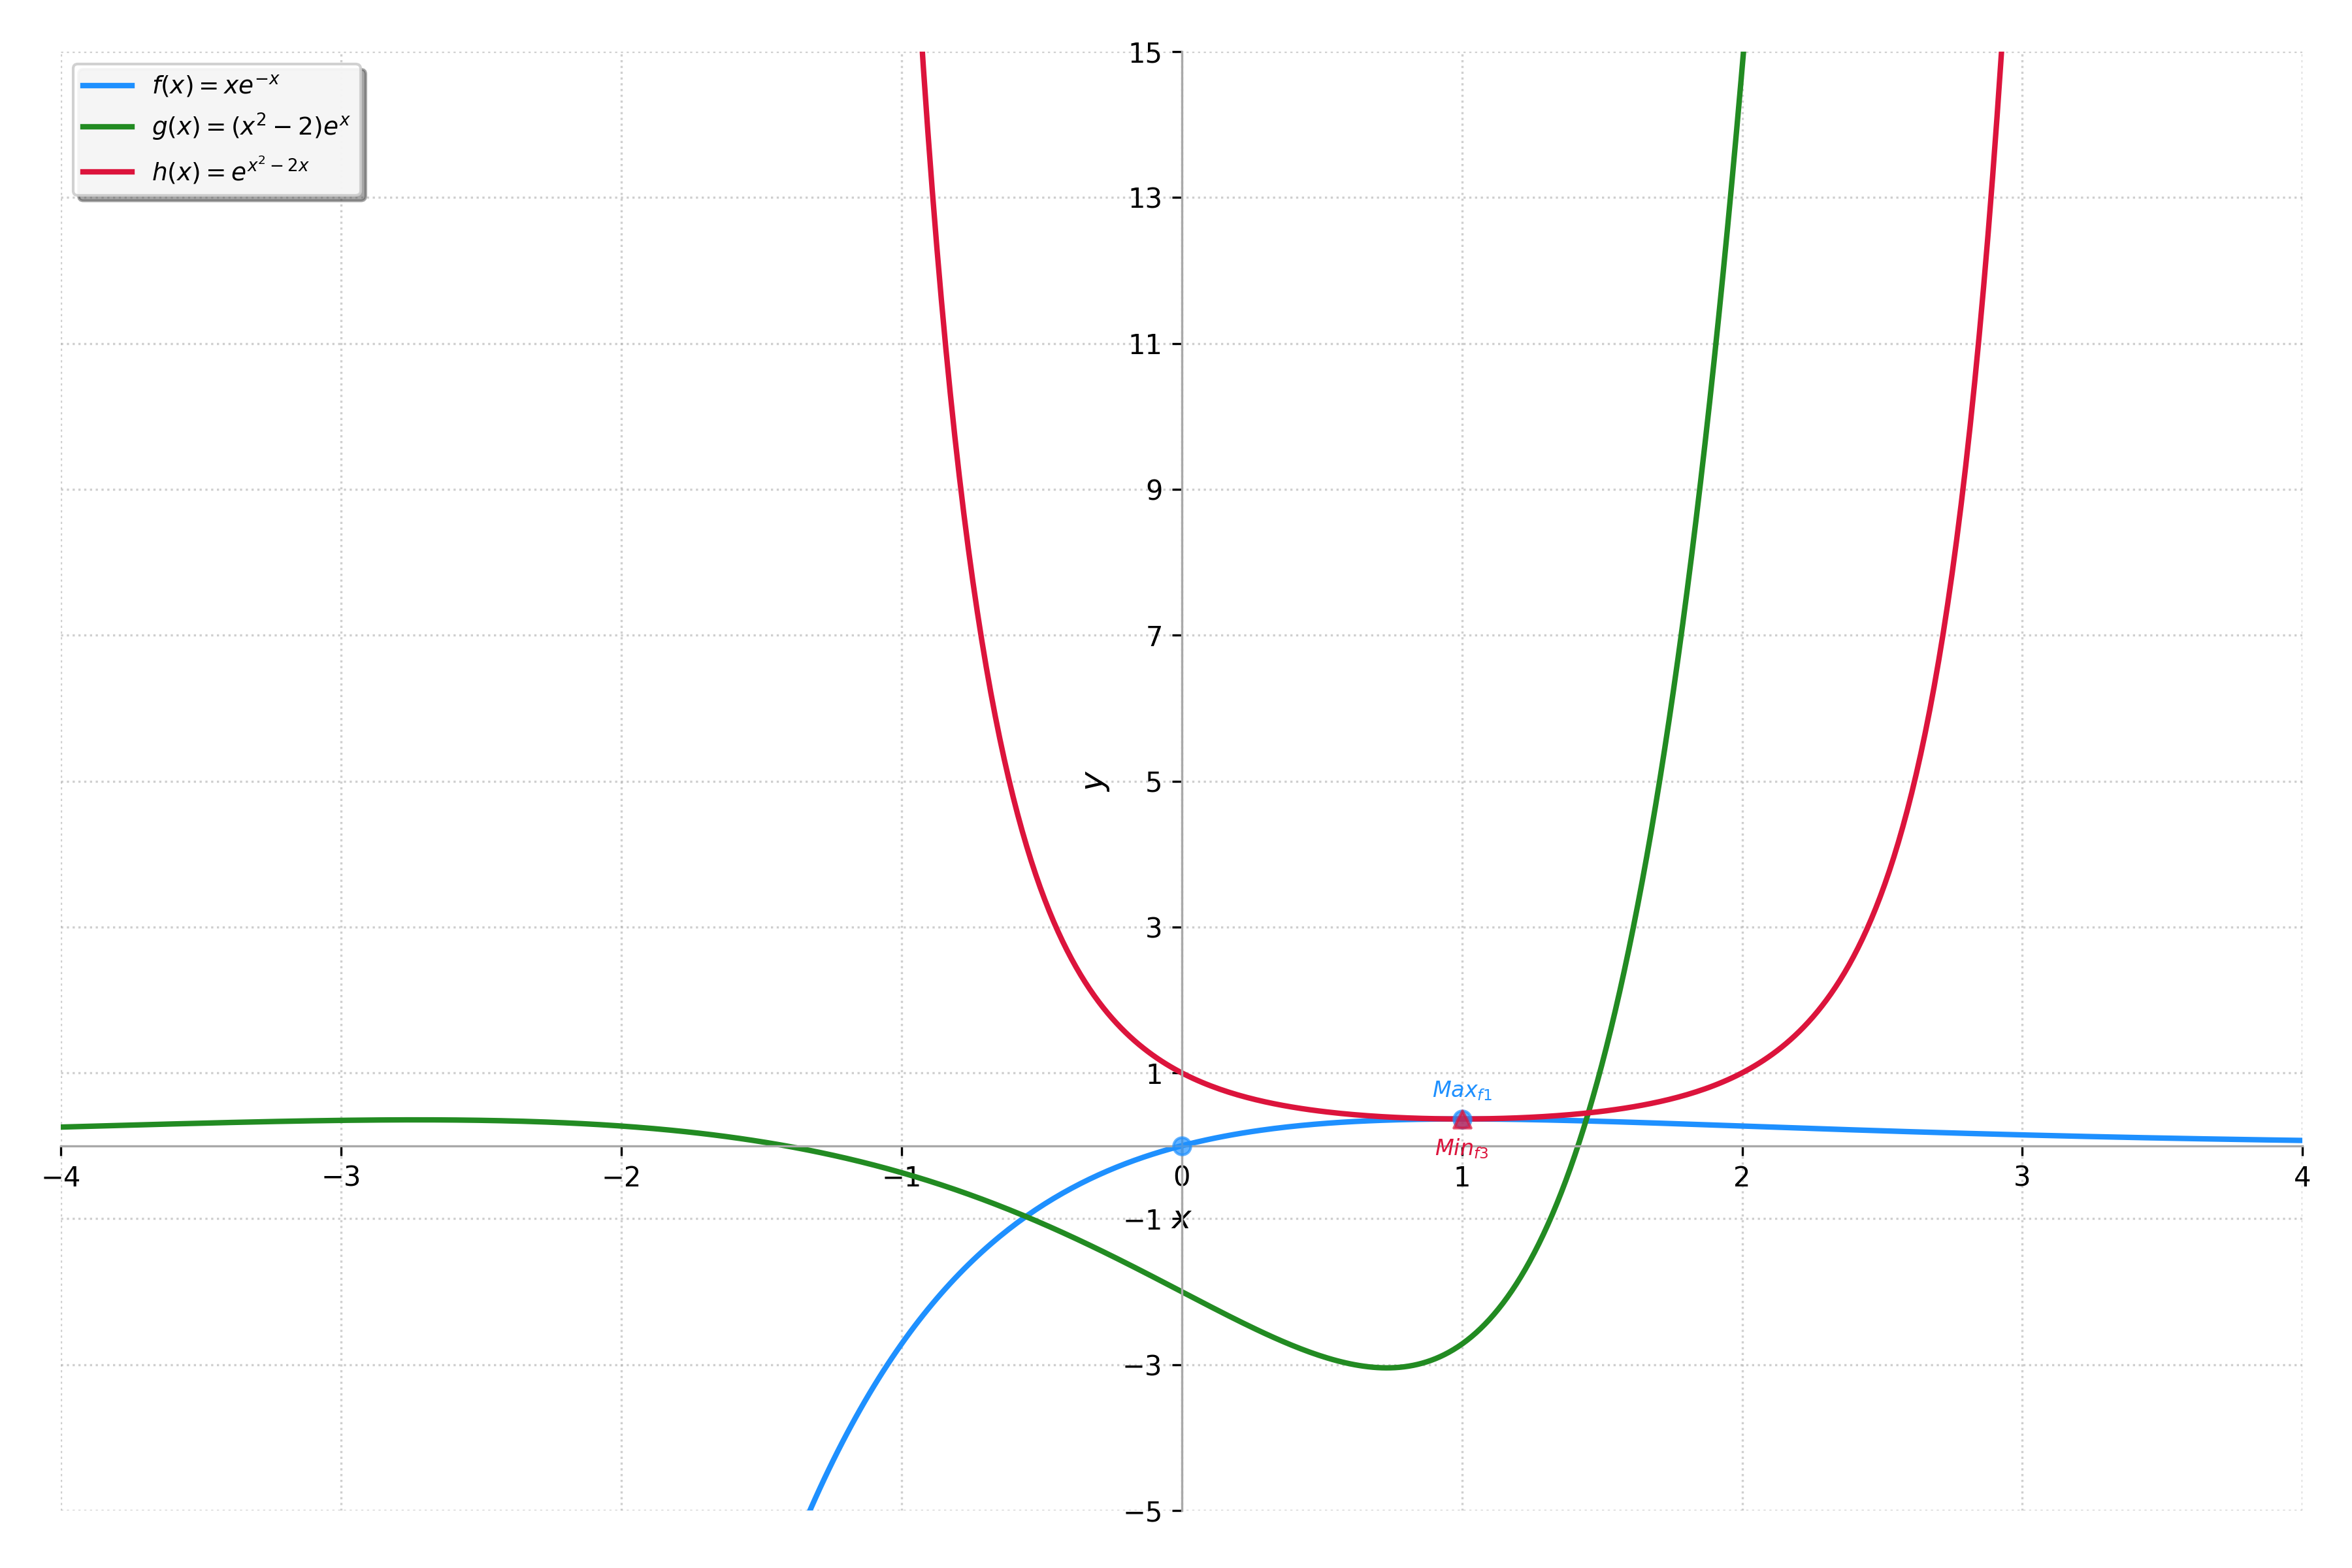
\includegraphics[width=0.8\textwidth]{grafiken/kurvendiskussion_ex_kombiniert.png}
% --- Beschreibung der Skizze ---
% Die Skizze sollte versuchen, die drei Graphen f(x), g(x), und h(x) darzustellen.
% f(x) = xe^{-x}: Charakteristischer Hügel im positiven Bereich, nähert sich der x-Achse für x -> unendlich.
% g(x) = (x^2-2)e^x: Nähert sich der x-Achse für x -> -unendlich, hat Nullstellen, ein lokales Maximum und Minimum.
% h(x) = e^{x^2-2x}: Parabelähnlicher Verlauf (obwohl es eine e-Funktion ist), mit Minimum bei (1, 1/e), steigt stark an für x -> +/- unendlich.
% Wegen der stark unterschiedlichen Wertebereiche und Verläufe ist eine einzelne übersichtliche Darstellung schwierig.
% Die x-Achse sollte zumindest den Bereich von ca. -4 bis 4 abdecken.
% Die y-Achse müsste einen Bereich von z.B. -4 bis 10 oder mehr abdecken, wobei Details von f(x) dann klein werden könnten.
\captionof{figure}{Skizze der Graphen von $f(x)$, $g(x)$ und $h(x)$ (konzeptionell).}
\label{fig:kurvendiskussion_ex_kombiniert}
\end{center}

\end{loesungsumgebung}




\begin{aufgabenumgebung}{Anwendung: Radioaktiver Zerfall}
Eine radioaktive Substanz zerfällt so, dass die noch vorhandene Menge $M(t)$ (in Gramm) nach $t$ Jahren durch die Funktion $M(t) = 100 \cdot e^{-0.05t}$ beschrieben wird.
\begin{enumerate}
    \item Wie groß ist die Anfangsmenge der Substanz?
    \item Wie viel Gramm sind nach 10 Jahren noch vorhanden?
    \item Mit welcher Rate zerfällt die Substanz zum Zeitpunkt $t=0$ und zum Zeitpunkt $t=10$ Jahre (in Gramm pro Jahr)? (Tipp: Ableitung $M'(t)$).
    \item \textbf{Halbwertszeit:} Nach welcher Zeit $T_H$ ist nur noch die Hälfte der ursprünglichen Menge vorhanden? (Setze $M(T_H) = \frac{1}{2}M(0)$ und löse nach $T_H$. Hierfür benötigst du den natürlichen Logarithmus $\ln$, die Umkehrfunktion von $e^x$.)
\end{enumerate}
\end{aufgabenumgebung}

\begin{loesungsumgebung}[loes:radioaktiver-zerfall-anwendung]{Anwendung: Radioaktiver Zerfall}
Die vorhandene Menge der Substanz $M(t)$ (in Gramm) nach $t$ Jahren ist gegeben durch $M(t) = 100 \cdot e^{-0.05t}$.

\begin{enumerate}[label=(\alph*)]
    \item \textbf{Wie groß ist die Anfangsmenge der Substanz?}
    Die Anfangsmenge ist die Menge zum Zeitpunkt $t=0$:
    $$ M(0) = 100 \cdot e^{-0.05 \cdot 0} = 100 \cdot e^0 = 100 \cdot 1 = 100 $$
    Die Anfangsmenge der Substanz beträgt \textbf{100 Gramm}.

    \item \textbf{Wie viel Gramm sind nach 10 Jahren noch vorhanden?}
    Wir setzen $t=10$ Jahre in die Funktion ein:
    $$ M(10) = 100 \cdot e^{-0.05 \cdot 10} = 100 \cdot e^{-0.5} $$
    Der exakte Wert ist $100e^{-0.5}$ Gramm.
    Näherungswert: $e^{-0.5} \approx 0.60653$.
    $$ M(10) \approx 100 \cdot 0.60653 = 60.653 $$
    Nach 10 Jahren sind noch ca. \textbf{60,65 Gramm} der Substanz vorhanden.

    \item \textbf{Mit welcher Rate zerfällt die Substanz zum Zeitpunkt $t=0$ und zum Zeitpunkt $t=10$ Jahre?}
    Die Zerfallsrate ist die erste Ableitung $M'(t)$ der Mengenfunktion.
    $M(t) = 100 e^{-0.05t}$.
    Mit der Kettenregel ($u(t)=-0.05t \Rightarrow u'(t)=-0.05$):
    $M'(t) = 100 \cdot e^{-0.05t} \cdot (-0.05) = -5e^{-0.05t}$.
    Die Einheit der Rate ist Gramm pro Jahr (g/Jahr). Das negative Vorzeichen zeigt an, dass die Menge abnimmt.

    \begin{itemize}
        \item \textbf{Zerfallsrate zum Zeitpunkt $t=0$ Jahre:}
        $M'(0) = -5e^{-0.05 \cdot 0} = -5e^0 = -5 \cdot 1 = -5$.
        Zum Zeitpunkt $t=0$ zerfällt die Substanz mit einer Rate von \textbf{5 Gramm pro Jahr}.
        \item \textbf{Zerfallsrate zum Zeitpunkt $t=10$ Jahre:}
        $M'(10) = -5e^{-0.05 \cdot 10} = -5e^{-0.5}$.
        $M'(10) \approx -5 \cdot 0.60653 \approx -3.03265$.
        Zum Zeitpunkt $t=10$ Jahre zerfällt die Substanz mit einer Rate von ca. \textbf{3,03 Gramm pro Jahr}.
    \end{itemize}

    \item \textbf{Halbwertszeit $T_H$:}
    Die Halbwertszeit ist die Zeit, nach der nur noch die Hälfte der ursprünglichen Menge vorhanden ist.
    Die Anfangsmenge ist $M(0) = 100\,$g. Die Hälfte davon ist $50\,$g.
    Wir setzen $M(T_H) = 50$:
    $$ 100 \cdot e^{-0.05 T_H} = 50 $$
    Wir lösen diese Gleichung nach $T_H$ auf:
    $$
    \begin{array}{r c l c l}
    \umformung{100 \cdot e^{-0.05 T_H}}{50}{\div}{100}
    \umformung{e^{-0.05 T_H}}{0.5}{\text{nimm } \ln(\dots)}{\text{auf beiden Seiten}}
    \umformung{\ln(e^{-0.05 T_H})}{\ln(0.5)}{}{ } % \ln(e^x)=x
    \umformung{-0.05 T_H}{\ln(0.5)}{\div}{(-0.05)}
    \umformungend{T_H}{\frac{\ln(0.5)}{-0.05}}
    \end{array}
    $$
    Da $\ln(0.5) = \ln(1/2) = \ln(1) - \ln(2) = 0 - \ln(2) = -\ln(2)$, können wir schreiben:
    $$ T_H = \frac{-\ln(2)}{-0.05} = \frac{\ln(2)}{0.05} $$
    Mit $\ln(2) \approx 0.693147$:
    $$ T_H \approx \frac{0.693147}{0.05} = 13.86294 $$
    Die Halbwertszeit beträgt $\mathbf{T_H = \frac{\ln 2}{0.05} \approx 13.86}$ Jahre.
\end{enumerate}

\end{loesungsumgebung}

\begin{aufgabenumgebung}{Optimierung im biologischen Kontext – Wachstum und Hemmung}
Eine Bakterienpopulation wächst zunächst, wird aber durch einen hemmenden Faktor (z.B. begrenzte Nährstoffe) beeinflusst. Die Anzahl der Bakterien $N$ (in Tausend) nach $t$ Stunden kann modelliert werden durch die Funktion:
\[ N(t) = 5t \cdot e^{-0.1t} \quad (\text{für } t \ge 0) \]
\begin{enumerate}
    \item \textbf{Anfangsbestand:} Wie viele Bakterien sind zum Zeitpunkt $t=0$ vorhanden? Interpretiere das Ergebnis im Kontext.
    \item \textbf{Wachstumsrate:} Bestimme die Funktion $N'(t)$, welche die Wachstumsrate der Bakterienpopulation zum Zeitpunkt $t$ angibt. (Produkt- und Kettenregel sind hier gefragt!)
    \item \textbf{Maximale Population:}
        \begin{itemize}
            \item Zu welchem Zeitpunkt $t_{max}$ erreicht die Bakterienpopulation ihr Maximum? (Tipp: Notwendige Bedingung für Extremstellen $N'(t)=0$. Da $e^{-0.1t}$ nie Null wird, musst du nur den anderen Faktor betrachten.)
            \item Überprüfe mit der zweiten Ableitung $N''(t)$ oder dem Vorzeichenwechselkriterium von $N'(t)$, ob es sich tatsächlich um ein Maximum handelt.
            \item Wie groß ist die maximale Bakterienpopulation $N(t_{max})$?
        \end{itemize}
    \item \textbf{Verhalten für $t \to \infty$:} Was passiert mit der Bakterienpopulation für sehr große Zeiten? (Untersuche $\lim_{t \to \infty} N(t)$). Ist das biologisch sinnvoll?
    \item \textbf{Stärkste Zunahme/Abnahme der Wachstumsrate (für Experten):}
        Die Änderungsrate der Wachstumsrate wird durch $N''(t)$ beschrieben. Wann ist die Zunahme der Wachstumsrate maximal (d.h. wann wächst die Population am schnellsten schneller)? Wann ist die Abnahme der Wachstumsrate maximal (d.h. wann verlangsamt sich das Wachstum am stärksten)? (Tipp: Untersuche $N''(t)$ auf Extremstellen, d.h. bilde $N'''(t)$).
    \item \textbf{Skizze:} Skizziere den Graphen von $N(t)$ für $t \ge 0$ und markiere den maximalen Bestand.
\end{enumerate}
\end{aufgabenumgebung}



\begin{loesungsumgebung}[loes:optimierung-bakterienwachstum]{Optimierung im biologischen Kontext – Wachstum und Hemmung}
Die Anzahl der Bakterien $N$ (in Tausend) nach $t$ Stunden wird modelliert durch $N(t) = 5t \cdot e^{-0.1t}$ für $t \ge 0$.

\begin{enumerate}[label=(\alph*)]
    \item \textbf{Anfangsbestand:}
    Der Anfangsbestand ist die Anzahl der Bakterien zum Zeitpunkt $t=0$:
    $$ N(0) = 5 \cdot 0 \cdot e^{-0.1 \cdot 0} = 0 \cdot e^0 = 0 \cdot 1 = 0 $$
    Zum Zeitpunkt $t=0$ sind \textbf{0 Tausend Bakterien} (also keine Bakterien laut Modell) vorhanden. Dies könnte bedeuten, dass die Beobachtung mit einer vernachlässigbar kleinen Startpopulation beginnt oder dass $t=0$ den Zeitpunkt unmittelbar vor Beginn des exponentiellen Wachstums darstellt, das dann durch die Hemmung beeinflusst wird.

    \item \textbf{Wachstumsrate $N'(t)$:}
    Die Wachstumsrate ist die erste Ableitung von $N(t)$. Wir verwenden die Produktregel: $u(t)=5t \Rightarrow u'(t)=5$; $v(t)=e^{-0.1t}$.
    Für $v'(t)$ verwenden wir die Kettenregel: $v'(t) = e^{-0.1t} \cdot (-0.1) = -0.1e^{-0.1t}$.
    \begin{align*}
    N'(t) &= u'(t)v(t) + u(t)v'(t) \\
           &= 5 \cdot e^{-0.1t} + 5t \cdot (-0.1e^{-0.1t}) \\
           &= 5e^{-0.1t} - 0.5te^{-0.1t} \\
           &= \mathbf{e^{-0.1t}(5 - 0.5t)}
    \end{align*}
    Die Einheit der Wachstumsrate ist Tausend Bakterien pro Stunde.

    \item \textbf{Maximale Population:}
    \begin{itemize}
        \item \textbf{Zeitpunkt $t_{max}$ der maximalen Population:}
        Wir setzen $N'(t)=0$: $e^{-0.1t}(5 - 0.5t) = 0$.
        Da $e^{-0.1t}$ stets positiv ist, muss der zweite Faktor Null sein:
        $5 - 0.5t = 0 \Rightarrow 0.5t = 5 \Rightarrow t = \frac{5}{0.5} = 10$.
        Der Zeitpunkt der potentiell maximalen Population ist $\mathbf{t_{max} = 10}$ Stunden.
        \item \textbf{Überprüfung mit der zweiten Ableitung $N''(t)$:}
        Wir leiten $N'(t) = 5e^{-0.1t} - 0.5te^{-0.1t}$ ab (Produktregel für den zweiten Term oder für die faktorisierte Form).
        Nehmen wir $N'(t) = e^{-0.1t}(5 - 0.5t)$.
        $u_2(t)=e^{-0.1t} \Rightarrow u_2'(t)=-0.1e^{-0.1t}$.
        $v_2(t)=5-0.5t \Rightarrow v_2'(t)=-0.5$.
        $N''(t) = u_2'(t)v_2(t) + u_2(t)v_2'(t)$
        $N''(t) = -0.1e^{-0.1t}(5 - 0.5t) + e^{-0.1t}(-0.5)$
        $N''(t) = e^{-0.1t}[-0.1(5 - 0.5t) - 0.5]$
        $N''(t) = e^{-0.1t}[-0.5 + 0.05t - 0.5] = e^{-0.1t}(0.05t - 1)$.
        Für $t=10$:
        $N''(10) = e^{-0.1 \cdot 10}(0.05 \cdot 10 - 1) = e^{-1}(0.5 - 1) = e^{-1}(-0.5) = -\frac{0.5}{e}$.
        Da $N''(10) < 0$, handelt es sich bei $t=10$ Stunden tatsächlich um ein lokales Maximum.
        \item \textbf{Maximale Bakterienpopulation $N(t_{max})$:}
        $N(10) = 5 \cdot 10 \cdot e^{-0.1 \cdot 10} = 50e^{-1} = \frac{50}{e}$.
        $N(10) \approx \frac{50}{2.71828} \approx 18.394$.
        Die maximale Population beträgt $\mathbf{\frac{50}{e} \approx 18.394}$ Tausend Bakterien (also ca. 18394 Bakterien).
    \end{itemize}

    \item \textbf{Verhalten für $t \to \infty$:}
    Wir untersuchen den Grenzwert der Populationsfunktion $N(t) = 5t e^{-0.1t} = \frac{5t}{e^{0.1t}}$ für $t \to \infty$.
    Da die Exponentialfunktion im Nenner schneller wächst als die lineare Funktion im Zähler, gilt (Standardgrenzwert):
    $$ \lim_{t \to \infty} \frac{5t}{e^{0.1t}} \stackrel{L'H}{=} \lim_{t \to \infty} \frac{5}{0.1e^{0.1t}} = \frac{5}{\infty} = 0 $$
    Für sehr große Zeiten nähert sich die Bakterienpopulation \textbf{Null} an.
    \textbf{Biologische Sinnhaftigkeit:} Dies ist biologisch sinnvoll. Auch wenn die Population anfangs wächst, führen begrenzte Nährstoffe, Anhäufung von Abfallprodukten oder andere limitierende Faktoren dazu, dass die Population nicht unbegrenzt wachsen kann und schließlich wieder abnimmt und ausstirbt oder ein sehr niedriges Niveau erreicht.

    \item \textbf{Stärkste Zunahme/Abnahme der Wachstumsrate (für Experten):}
    Die Wachstumsrate ist $N'(t) = e^{-0.1t}(5 - 0.5t)$. Die Änderungsrate der Wachstumsrate ist $N''(t) = e^{-0.1t}(0.05t - 1)$. Wir suchen die Extrema von $N''(t)$. Dazu bilden wir die Ableitung von $N''(t)$, also $N'''(t)$.
    $N'''(t) = \frac{d}{dt} [e^{-0.1t}(0.05t - 1)]$.
    Mit $u(t)=e^{-0.1t} \Rightarrow u'(t)=-0.1e^{-0.1t}$ und $v(t)=0.05t-1 \Rightarrow v'(t)=0.05$.
    $N'''(t) = -0.1e^{-0.1t}(0.05t - 1) + e^{-0.1t}(0.05)$
    $N'''(t) = e^{-0.1t}[-0.1(0.05t - 1) + 0.05]$
    $N'''(t) = e^{-0.1t}[-0.005t + 0.1 + 0.05] = e^{-0.1t}(-0.005t + 0.15)$.
    Setze $N'''(t)=0$ für kritische Stellen von $N''(t)$:
    $e^{-0.1t}(-0.005t + 0.15) = 0$.
    Da $e^{-0.1t} \neq 0$, muss $-0.005t + 0.15 = 0 \Rightarrow 0.005t = 0.15 \Rightarrow t = \frac{0.15}{0.005} = \frac{150}{5} = 30$.
    Um die Art des Extremums von $N''(t)$ bei $t=30$ zu bestimmen, bilden wir $N^{(4)}(t)$:
    $N^{(4)}(t) = \frac{d}{dt} [e^{-0.1t}(-0.005t + 0.15)]$.
    Mit $u(t)=e^{-0.1t} \Rightarrow u'(t)=-0.1e^{-0.1t}$ und $v(t)=-0.005t+0.15 \Rightarrow v'(t)=-0.005$.
    $N^{(4)}(t) = -0.1e^{-0.1t}(-0.005t + 0.15) + e^{-0.1t}(-0.005)$
    $N^{(4)}(t) = e^{-0.1t}[-0.1(-0.005t + 0.15) - 0.005] = e^{-0.1t}[0.0005t - 0.015 - 0.005] = e^{-0.1t}(0.0005t - 0.02)$.
    $N^{(4)}(30) = e^{-3}(0.0005 \cdot 30 - 0.02) = e^{-3}(0.015 - 0.02) = e^{-3}(-0.005)$.
    Da $N^{(4)}(30) < 0$, hat $N''(t)$ bei $t=30$ ein \textbf{lokales Maximum}.
    $N''(30) = e^{-0.1 \cdot 30}(0.05 \cdot 30 - 1) = e^{-3}(1.5 - 1) = 0.5e^{-3} \approx 0.0249 > 0$.
    Die Zunahme der Wachstumsrate ist also bei $\mathbf{t=30}$ Stunden maximal (d.h. das Wachstum beschleunigt sich dort am stärksten positiv).
    Um die stärkste Abnahme der Wachstumsrate zu finden (wo $N''(t)$ am negativsten ist), betrachten wir die Ränder des sinnvollen Definitionsbereichs und andere kritische Punkte, falls vorhanden. $N''(t) = e^{-0.1t}(0.05t - 1)$.
    $N''(0) = e^0(0-1) = -1$.
    Die Nullstelle von $N''(t)$ ist bei $t=20$.
    Für $0 \le t < 20$: $0.05t-1 < 0 \Rightarrow N''(t) < 0$ (Wachstumsrate nimmt ab).
    Für $t > 20$: $0.05t-1 > 0 \Rightarrow N''(t) > 0$ (Wachstumsrate nimmt zu, bis $t=30$, dann wird Zunahme der Zunahme geringer).
    Das Minimum von $N''(t)$ im Intervall $t \ge 0$ tritt also bei $t=0$ auf.
    Die Abnahme der Wachstumsrate ist maximal (d.h. $N''(t)$ ist am negativsten) bei $\mathbf{t=0}$ Stunden, mit $N''(0) = -1$. (Hier verlangsamt sich das Wachstum am stärksten, bzw. die anfängliche 'Bremsung' des Wachstums ist am stärksten, da $N'(0)=5$ positiv ist, aber $N''(0)=-1$ negativ).
\end{enumerate}

\end{loesungsumgebung}



\begin{aufgabenumgebung}{Tangenten an Exponentialfunktionen}
Gegeben ist die Funktion $f(x) = (x-2)e^x$.
\begin{enumerate}
    \item Bestimme die Gleichung der Tangente an den Graphen von $f$ im Punkt $P(2|f(2))$.
    \item In welchem Punkt schneidet diese Tangente die y-Achse?
    \item Gibt es eine Stelle $x_0$, an der die Tangente an den Graphen von $f$ parallel zur x-Achse verläuft? Wenn ja, bestimme $x_0$ und die Art des Extrempunktes an dieser Stelle.
    \item (Für Experten): Gibt es eine Tangente an den Graphen von $f$, die durch den Ursprung $(0|0)$ verläuft, aber nicht im Ursprung berührt?

\end{enumerate}
\end{aufgabenumgebung}


\begin{loesungsumgebung}[loes:tangenten-ex-funktionen]{Tangenten an Exponentialfunktionen}
Gegeben ist die Funktion $f(x) = (x-2)e^x$.
Die erste Ableitung $f'(x)$ bestimmen wir mit der Produktregel:
Sei $u(x) = x-2 \Rightarrow u'(x) = 1$.
Sei $v(x) = e^x \Rightarrow v'(x) = e^x$.
$f'(x) = u'(x)v(x) + u(x)v'(x) = 1 \cdot e^x + (x-2)e^x = e^x(1 + x - 2) = (x-1)e^x$.

\begin{enumerate}[label=(\alph*)]
    \item \textbf{Gleichung der Tangente und der Normalen an den Graphen von $f$ im Punkt $P(2|f(2))$.}
    \begin{itemize}
        \item Zuerst bestimmen wir die y-Koordinate des Punktes $P$:
        $f(2) = (2-2)e^2 = 0 \cdot e^2 = 0$. Der Berührpunkt ist also $P(2|0)$.
        \item Die Steigung der Tangente $m_t$ im Punkt $P(2|0)$ ist $f'(2)$:
        $m_t = f'(2) = (2-1)e^2 = 1 \cdot e^2 = e^2$.
        \item Die Gleichung der Tangente $y_t = m_t(x-x_0) + y_0$ ist:
        $y_t = e^2(x-2) + 0 \Rightarrow \mathbf{y_t = e^2x - 2e^2}$.
        % Für die Normale (nicht explizit gefragt, aber oft Teil solcher Aufgaben):
        % Die Steigung der Normalen $m_n = -1/m_t = -1/e^2$.
        % Normalengleichung: $y_n - 0 = -\frac{1}{e^2}(x-2) \Rightarrow y_n = -\frac{1}{e^2}x + \frac{2}{e^2}$.
    \end{itemize}

    \item \textbf{In welchem Punkt schneidet diese Tangente die y-Achse?}
    Die Tangentengleichung ist $y_t = e^2x - 2e^2$.
    Um den Schnittpunkt mit der y-Achse zu finden, setzen wir $x=0$:
    $y_t(0) = e^2(0) - 2e^2 = -2e^2$.
    Der Schnittpunkt mit der y-Achse ist $\mathbf{P_y(0|-2e^2)}$.

    \item \textbf{Gibt es eine Stelle $x_0$, an der die Tangente an den Graphen von $f$ parallel zur x-Achse verläuft? Wenn ja, bestimme $x_0$ und die Art des Extrempunktes an dieser Stelle.}
    Eine Tangente ist parallel zur x-Achse, wenn ihre Steigung Null ist, d.h. $f'(x_0)=0$.
    $f'(x_0) = (x_0-1)e^{x_0} = 0$.
    Da $e^{x_0}$ immer positiv ist ($e^{x_0} > 0$), muss gelten:
    $x_0-1 = 0 \Rightarrow \mathbf{x_0 = 1}$.
    Um die Art des Extrempunktes zu bestimmen, bilden wir die zweite Ableitung $f''(x)$:
    $f'(x) = (x-1)e^x$. Mit Produktregel ($u=x-1, u'=1; v=e^x, v'=e^x$):
    $f''(x) = 1 \cdot e^x + (x-1)e^x = e^x(1+x-1) = xe^x$.
    An der Stelle $x_0=1$:
    $f''(1) = 1 \cdot e^1 = e$.
    Da $f''(1) = e > 0$, liegt bei $x_0=1$ ein \textbf{lokaler Tiefpunkt} vor.
    Die y-Koordinate ist $f(1) = (1-2)e^1 = -e$.
    Der Tiefpunkt ist $TP(1|-e)$.

    \item \textbf{(Für Experten): Gibt es eine Tangente an den Graphen von $f$, die durch den Ursprung $(0|0)$ verläuft, aber nicht im Ursprung berührt?}
    Der Punkt $(0|0)$ liegt nicht auf dem Graphen von $f$, da $f(0) = (0-2)e^0 = -2 \neq 0$. Also suchen wir eine Tangente von einem externen Punkt $(0|0)$ an den Graphen.
    Sei $B(x_B | f(x_B))$ der Berührpunkt der Tangente am Graphen. Die Steigung der Tangente in $B$ ist $m_T = f'(x_B) = (x_B-1)e^{x_B}$.
    Die Steigung der Geraden durch den Ursprung $O(0|0)$ und den Berührpunkt $B(x_B | f(x_B))$ ist (für $x_B \neq 0$):
    $m_{OB} = \frac{f(x_B) - 0}{x_B - 0} = \frac{(x_B-2)e^{x_B}}{x_B}$.
    Für eine Tangente müssen diese Steigungen gleich sein: $m_T = m_{OB}$.
    $$ (x_B-1)e^{x_B} = \frac{(x_B-2)e^{x_B}}{x_B} $$
    Da $e^{x_B} \neq 0$, können wir dadurch teilen:
    $$ x_B-1 = \frac{x_B-2}{x_B} $$
    Multiplikation mit $x_B$ (wir suchen einen Berührpunkt $x_B \neq 0$, da sonst der Nenner Null wäre und der Ursprung kein Berührpunkt ist, da $f(0) \neq 0$):
    $$ x_B(x_B-1) = x_B-2 $$
    $$ x_B^2 - x_B = x_B - 2 $$
    $$ x_B^2 - 2x_B + 2 = 0 $$
    Wir untersuchen die Diskriminante dieser quadratischen Gleichung ($a=1, b=-2, c=2$):
    $D = b^2 - 4ac = (-2)^2 - 4(1)(2) = 4 - 8 = -4$.
    Da die Diskriminante $D < 0$ ist, hat die quadratische Gleichung keine reellen Lösungen für $x_B$.
    \textbf{Schlussfolgerung:} Es gibt keine solche Stelle $x_B$ und somit keine Tangente an den Graphen von $f(x)$, die durch den Ursprung $(0|0)$ verläuft (und nicht im Ursprung berührt, was ohnehin nicht der Fall ist, da $f(0)\neq0$).
\end{enumerate}

\end{loesungsumgebung}

\begin{aufgabenumgebung}{Kurvendiskussion einer komplexeren e-Funktion}
Führe eine vollständige Kurvendiskussion für die Funktion $f(x) = (x^2 - 3)e^{-x}$ durch. Untersuche dabei insbesondere:
\begin{itemize}
    \item Definitionsbereich, Symmetrie
    \item Verhalten im Unendlichen (Grenzwerte, Asymptoten)
    \item Nullstellen
    \item Extrempunkte (Lage und Art)
    \item Wendepunkte (Lage)
    \item Skizziere den Graphen von $f(x)$.
\end{itemize}
\end{aufgabenumgebung}

\begin{loesungsumgebung}[loes:kurvendiskussion-komplex-ex]{Kurvendiskussion einer komplexeren e-Funktion}
Wir führen eine vollständige Kurvendiskussion für die Funktion $f(x) = (x^2 - 3)e^{-x}$ durch.

\subsubsection*{1. Definitionsbereich ($D_f$)}
Die Terme $x^2-3$ und $e^{-x}$ sind für alle reellen Zahlen definiert.
Somit ist der Definitionsbereich $\mathbf{D_f = \mathbb{R}}$.

\subsubsection*{2. Symmetrie}
Wir untersuchen $f(-x)$:
$f(-x) = ((-x)^2 - 3)e^{-(-x)} = (x^2 - 3)e^x$.
Da $f(-x) \neq f(x)$ und $f(-x) \neq -f(x)$ (z.B. $f(1) = (1-3)e^{-1} = -2e^{-1}$, während $f(-1) = (1-3)e^1 = -2e$, und $-f(1) = 2e^{-1}$), liegt \textbf{keine einfache Achsen- oder Punktsymmetrie} zum Ursprung vor.

\subsubsection*{3. Verhalten im Unendlichen (Grenzwerte, Asymptoten)}
\begin{itemize}
    \item Für $x \to \infty$:
    $f(x) = \frac{x^2 - 3}{e^x}$. Da die Exponentialfunktion $e^x$ schneller wächst als jede Potenz von $x$, gilt:
    $$ \lim_{x \to \infty} \frac{x^2 - 3}{e^x} = 0 $$
    (Dies kann auch zweimal mit der Regel von L'Hôpital gezeigt werden: $\lim_{x \to \infty} \frac{2x}{e^x} = \lim_{x \to \infty} \frac{2}{e^x} = 0$).
    Somit hat die Funktion eine \textbf{horizontale Asymptote $y=0$} für $x \to \infty$.
    \item Für $x \to -\infty$:
    Sei $u = -x$. Wenn $x \to -\infty$, dann $u \to \infty$.
    $f(x) = ((-u)^2 - 3)e^{-(-u)} = (u^2 - 3)e^u$.
    $$ \lim_{u \to \infty} (u^2 - 3)e^u = (\infty - 3) \cdot \infty = \infty \cdot \infty = \infty $$
    Also $\lim_{x \to -\infty} f(x) = \mathbf{\infty}$.
\end{itemize}

\subsubsection*{4. Achsenschnittpunkte}
\begin{itemize}
    \item \textbf{Schnittpunkt mit der y-Achse} (setze $x=0$):
    $f(0) = (0^2 - 3)e^0 = (-3) \cdot 1 = -3$.
    Der y-Achsenabschnitt ist $P_y(0|-3)$.
    \item \textbf{Nullstellen} (setze $f(x)=0$):
    $(x^2 - 3)e^{-x} = 0$.
    Da $e^{-x} > 0$ für alle $x \in \mathbb{R}$, muss $x^2 - 3 = 0$ sein.
    $x^2 = 3 \Rightarrow x = \pm\sqrt{3}$.
    Die Nullstellen sind $\mathbf{x_{N1} = -\sqrt{3} \approx -1.732}$ und $\mathbf{x_{N2} = \sqrt{3} \approx 1.732}$.
\end{itemize}

\subsubsection*{5. Erste Ableitung $f'(x)$}
Wir verwenden die Produktregel ($u=x^2-3, v=e^{-x}$):
$u'(x) = 2x$.
$v'(x) = -e^{-x}$.
\begin{align*}
f'(x) &= u'(x)v(x) + u(x)v'(x) \\
      &= 2x \cdot e^{-x} + (x^2-3) \cdot (-e^{-x}) \\
      &= e^{-x} [2x - (x^2-3)] \\
      &= e^{-x} (2x - x^2 + 3) \\
      &= \mathbf{(-x^2 + 2x + 3)e^{-x}}
\end{align*}

\subsubsection*{6. Extrempunkte (Lage und Art)}
Notwendige Bedingung: $f'(x_E)=0$.
$(-x^2 + 2x + 3)e^{-x} = 0$.
Da $e^{-x} \neq 0$, muss $-x^2 + 2x + 3 = 0 \Rightarrow x^2 - 2x - 3 = 0$.
Diese quadratische Gleichung lässt sich faktorisieren: $(x-3)(x+1)=0$.
Die kritischen Stellen sind $x_{E1} = -1$ und $x_{E2} = 3$.
Hinreichende Bedingung: Wir untersuchen das Vorzeichen von $f'(x)$. Der Faktor $e^{-x}$ ist immer positiv. Das Vorzeichen von $f'(x)$ wird also durch $P(x) = -x^2+2x+3$ bestimmt. Dies ist eine nach unten geöffnete Parabel mit Nullstellen bei $-1$ und $3$.
\begin{itemize}
    \item Für $x < -1$ (z.B. $x=-2$): $P(-2) = -4-4+3 = -5 < 0 \Rightarrow f'(x) < 0$.
    \item Für $-1 < x < 3$ (z.B. $x=0$): $P(0) = 3 > 0 \Rightarrow f'(x) > 0$.
    \item Für $x > 3$ (z.B. $x=4$): $P(4) = -16+8+3 = -5 < 0 \Rightarrow f'(x) < 0$.
\end{itemize}
Daraus folgt:
\begin{itemize}
    \item Bei $x_{E1} = -1$: Vorzeichenwechsel von $f'(x)$ von $-$ nach $+ \Rightarrow$ \textbf{Lokaler Tiefpunkt}.
    $y_{E1} = f(-1) = ((-1)^2-3)e^{-(-1)} = (1-3)e^1 = -2e \approx -5.437$.
    $\mathbf{TP(-1|-2e)}$.
    \item Bei $x_{E2} = 3$: Vorzeichenwechsel von $f'(x)$ von $+$ nach $- \Rightarrow$ \textbf{Lokaler Hochpunkt}.
    $y_{E2} = f(3) = ((3)^2-3)e^{-3} = (9-3)e^{-3} = 6e^{-3} = \frac{6}{e^3} \approx 0.299$.
    $\mathbf{HP(3|6e^{-3})}$.
\end{itemize}

\subsubsection*{7. Monotonieverhalten}
Aus der Untersuchung von $f'(x)$:
\begin{itemize}
    \item Streng monoton fallend in $(-\infty, -1]$.
    \item Streng monoton steigend in $[-1, 3]$.
    \item Streng monoton fallend in $[3, \infty)$.
\end{itemize}

\subsubsection*{8. Zweite Ableitung $f''(x)$}
Wir leiten $f'(x) = (-x^2 + 2x + 3)e^{-x}$ mit der Produktregel ab:
$u(x) = -x^2+2x+3 \Rightarrow u'(x) = -2x+2$.
$v(x) = e^{-x} \Rightarrow v'(x) = -e^{-x}$.
\begin{align*}
f''(x) &= (-2x+2)e^{-x} + (-x^2+2x+3)(-e^{-x}) \\
       &= e^{-x} [(-2x+2) - (-x^2+2x+3)] \\
       &= e^{-x} [-2x+2 + x^2-2x-3] \\
       &= \mathbf{(x^2 - 4x - 1)e^{-x}}
\end{align*}

\subsubsection*{9. Wendepunkte (Lage)}
Notwendige Bedingung: $f''(x_W)=0$.
$(x^2 - 4x - 1)e^{-x} = 0$.
Da $e^{-x} \neq 0$, muss $x^2 - 4x - 1 = 0$.
Mit der Mitternachtsformel: $x_W = \frac{-(-4) \pm \sqrt{(-4)^2 - 4(1)(-1)}}{2(1)} = \frac{4 \pm \sqrt{16+4}}{2} = \frac{4 \pm \sqrt{20}}{2}$.
$\sqrt{20} = \sqrt{4 \cdot 5} = 2\sqrt{5}$.
$x_W = \frac{4 \pm 2\sqrt{5}}{2} = 2 \pm \sqrt{5}$.
Die potentiellen Wendestellen sind $x_{W1} = 2 - \sqrt{5} \approx -0.236$ und $x_{W2} = 2 + \sqrt{5} \approx 4.236$.
Hinreichende Bedingung: Wir prüfen, ob $f'''(x_W) \neq 0$ oder ob $f''(x)$ das Vorzeichen wechselt. Da $x^2-4x-1$ eine Parabel ist, die ihre Nullstellen schneidet, wechselt $f''(x)$ das Vorzeichen an diesen Stellen. Somit liegen Wendepunkte vor.
y-Koordinaten:
$y_{W1} = f(2-\sqrt{5}) = ((2-\sqrt{5})^2-3)e^{-(2-\sqrt{5})} = (4-4\sqrt{5}+5-3)e^{\sqrt{5}-2} = (6-4\sqrt{5})e^{\sqrt{5}-2} \approx -3.727$.
$y_{W2} = f(2+\sqrt{5}) = ((2+\sqrt{5})^2-3)e^{-(2+\sqrt{5})} = (4+4\sqrt{5}+5-3)e^{-2-\sqrt{5}} = (6+4\sqrt{5})e^{-2-\sqrt{5}} \approx 0.216$.
Wendepunkte: $\mathbf{WP_1(2-\sqrt{5} | (6-4\sqrt{5})e^{\sqrt{5}-2})}$ und $\mathbf{WP_2(2+\sqrt{5} | (6+4\sqrt{5})e^{-2-\sqrt{5}})}$.

\subsubsection*{10. Krümmungsverhalten}
Das Vorzeichen von $f''(x) = (x^2 - 4x - 1)e^{-x}$ wird durch den quadratischen Term $P(x)=x^2-4x-1$ bestimmt (da $e^{-x}>0$). $P(x)$ ist eine nach oben geöffnete Parabel mit Nullstellen $x_{W1}$ und $x_{W2}$.
\begin{itemize}
    \item Für $x < 2-\sqrt{5}$: $P(x) > 0 \Rightarrow f''(x) > 0 \Rightarrow f(x)$ ist linksgekrümmt (konvex).
    \item Für $2-\sqrt{5} < x < 2+\sqrt{5}$: $P(x) < 0 \Rightarrow f''(x) < 0 \Rightarrow f(x)$ ist rechtsgekrümmt (konkav).
    \item Für $x > 2+\sqrt{5}$: $P(x) > 0 \Rightarrow f''(x) > 0 \Rightarrow f(x)$ ist linksgekrümmt (konvex).
\end{itemize}

\subsubsection*{11. Wertebereich ($W_f$)}
Der globale Tiefpunkt ist $TP(-1|-2e \approx -5.437)$. Der Graph geht für $x \to -\infty$ nach $\infty$. Der Hochpunkt ist $HP(3|6e^{-3} \approx 0.299)$ und für $x \to \infty$ geht $f(x) \to 0$.
Somit ist der Wertebereich $\mathbf{W_f = [-2e, \infty)}$.

\subsubsection*{12. Skizze des Graphen}
Der Graph startet im Unendlichen für $x \to -\infty$, fällt zu einem Tiefpunkt bei $TP(-1|-2e)$, steigt dann an, durchläuft einen Wendepunkt bei $WP_1(2-\sqrt{5}| \dots)$, schneidet die y-Achse bei $(0|-3)$, steigt weiter zu einem Hochpunkt bei $HP(3|6e^{-3})$, fällt dann, durchläuft einen weiteren Wendepunkt bei $WP_2(2+\sqrt{5}| \dots)$ und nähert sich der x-Achse ($y=0$) als Asymptote für $x \to \infty$. Die Nullstellen sind bei $x=\pm\sqrt{3}$.
\begin{center}
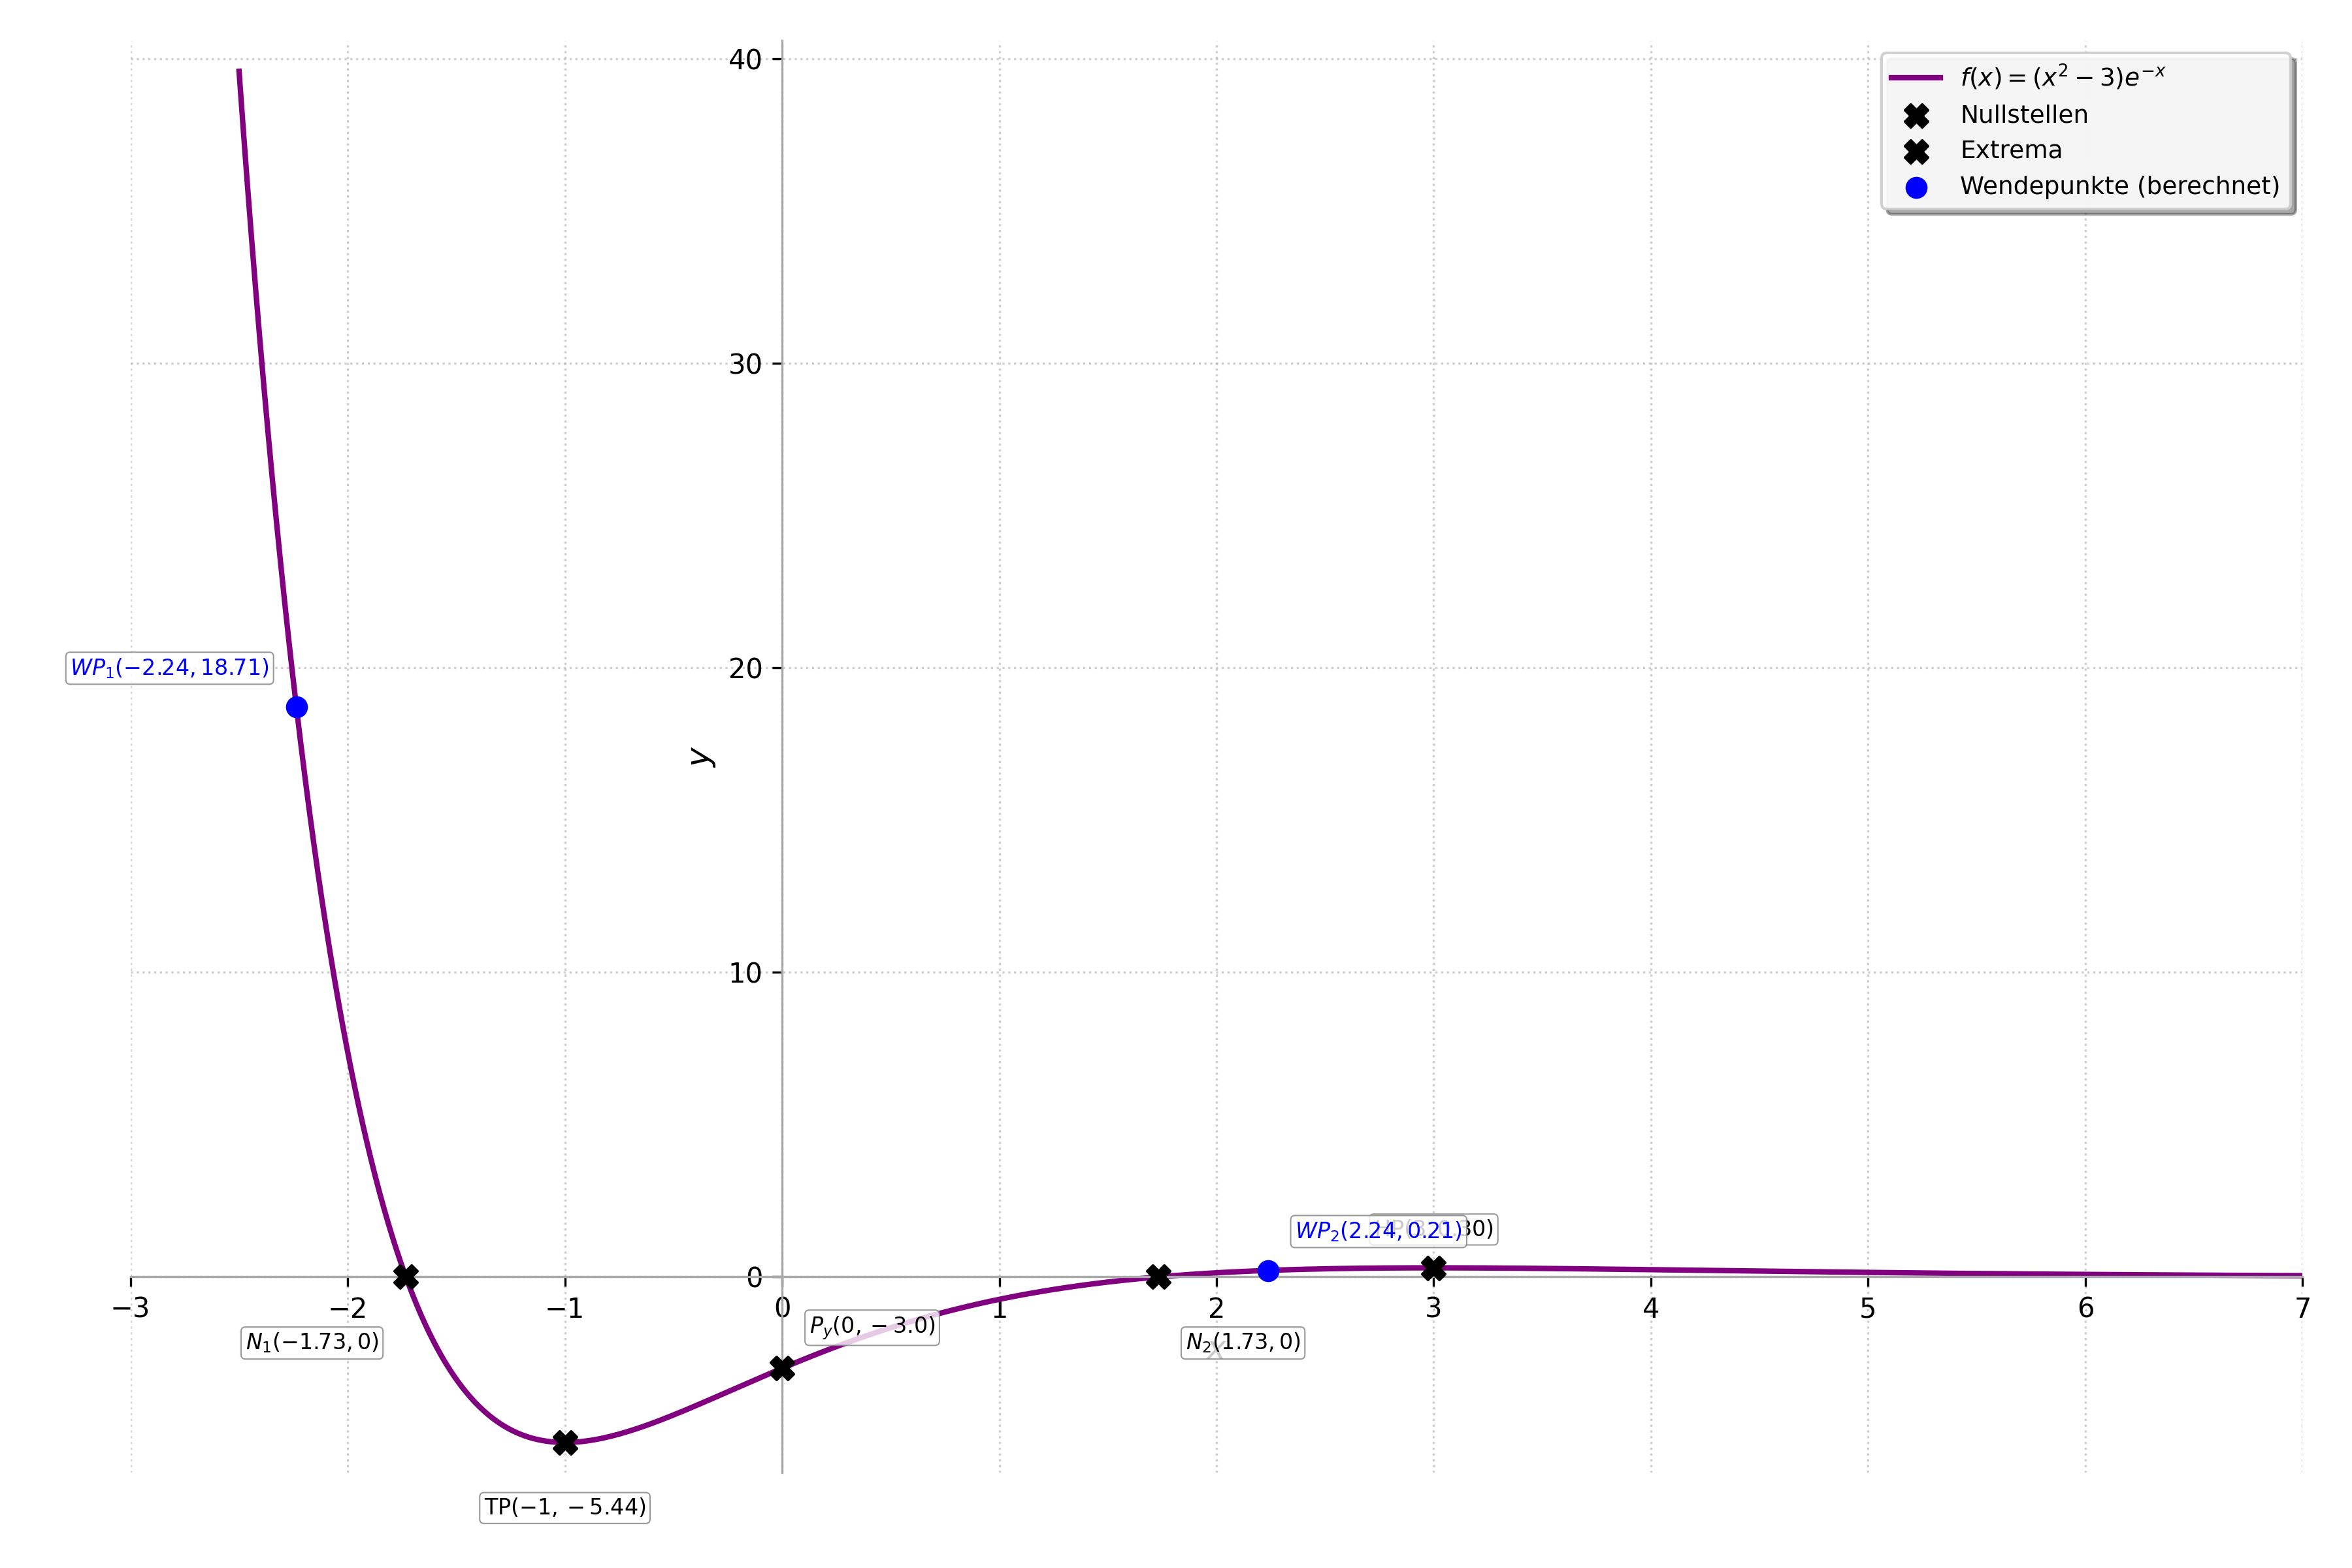
\includegraphics[width=0.8\textwidth]{grafiken/kurvendisk_komplex_ex.png}
% --- Beschreibung der Skizze ---
% Die Skizze zeigt einen Graphen, der von links oben aus dem Unendlichen kommt.
% Er schneidet die x-Achse bei x = -sqrt(3) (ca. -1.73).
% Erreicht einen Tiefpunkt bei TP(-1 | -2e) (ca. -1 | -5.44).
% Steigt an, durchläuft einen Wendepunkt bei WP1(2-sqrt(5) | ...) (ca. -0.24 | -3.73).
% Schneidet die y-Achse bei (0 | -3).
% Steigt weiter zu einem Hochpunkt bei HP(3 | 6e^-3) (ca. 3 | 0.30).
% Fällt dann ab, schneidet die x-Achse bei x = sqrt(3) (ca. 1.73).
% Durchläuft einen Wendepunkt bei WP2(2+sqrt(5) | ...) (ca. 4.24 | 0.22).
% Nähert sich der x-Achse (y=0) asymptotisch für x -> +unendlich.
\captionof{figure}{Graph der Funktion $f(x) = (x^2 - 3)e^{-x}$.}
\label{fig:kurvendisk_komplex_ex}
\end{center}

\end{loesungsumgebung}

\begin{aufgabenumgebung}{Partielle Integration üben – Mehr Vielfalt}
Berechne die folgenden unbestimmten Integrale mit partieller Integration:
\begin{enumerate}
    \item $\int (2x+1)e^x \,dx$
    \item $\int x^2 e^x \,dx$ (Tipp: Hier musst du die partielle Integration zweimal anwenden!)
    \item $\int \ln(x) \,dx$
    \item $\int x \cos(x) \,dx$
    \item $\int (x^2+1)\ln(x) \,dx$
    \item \textbf{Herausforderung (das 'Trick-Integral'):} $\int e^x \sin(x) \,dx$

\end{enumerate}
\end{aufgabenumgebung}

\begin{loesungsumgebung}[loes:partielle-integration-ueben-vielfalt]{Partielle Integration üben – Mehr Vielfalt}
Wir berechnen die unbestimmten Integrale mithilfe der partiellen Integration.

\begin{enumerate}[label=(\alph*)]
    \item $\mathbf{\int (2x+1)e^x \,dx}$ \\
    Wir wählen:
    \begin{itemize}
        \item $f(x) = 2x+1 \Rightarrow f'(x) = 2$ (wird einfacher beim Ableiten)
        \item $g'(x) = e^x \Rightarrow g(x) = e^x$ (leicht zu integrieren)
    \end{itemize}
    Anwendung der Formel $\int f(x)g'(x) \,dx = f(x)g(x) - \int f'(x)g(x) \,dx$:
    \begin{align*} \int (2x+1)e^x \,dx &= (2x+1)e^x - \int 2e^x \,dx \\ &= (2x+1)e^x - 2\int e^x \,dx \\ &= (2x+1)e^x - 2e^x + C \\ &= e^x(2x+1-2) + C \\ &= \mathbf{e^x(2x-1) + C} \end{align*}

    \item $\mathbf{\int x^2 e^x \,dx}$ (Tipp: Zweimal anwenden) \\
    \textbf{Erste partielle Integration:}
    Wir wählen:
    \begin{itemize}
        \item $f(x) = x^2 \Rightarrow f'(x) = 2x$
        \item $g'(x) = e^x \Rightarrow g(x) = e^x$
    \end{itemize}
    $$ \int x^2 e^x \,dx = x^2e^x - \int 2x e^x \,dx = x^2e^x - 2 \int x e^x \,dx \quad (*) $$
    \textbf{Zweite partielle Integration für $\int x e^x \,dx$:}
    Wir wählen für dieses Integral:
    \begin{itemize}
        \item $f_2(x) = x \Rightarrow f_2'(x) = 1$
        \item $g_2'(x) = e^x \Rightarrow g_2(x) = e^x$
    \end{itemize}
    $$ \int x e^x \,dx = xe^x - \int 1 \cdot e^x \,dx = xe^x - e^x $$
    Setzen wir dies zurück in $(*)$:
    \begin{align*} \int x^2 e^x \,dx &= x^2e^x - 2(xe^x - e^x) + C \\ &= x^2e^x - 2xe^x + 2e^x + C \\ &= \mathbf{e^x(x^2 - 2x + 2) + C} \end{align*}

    \item $\mathbf{\int \ln(x) \,dx}$ \\
    Tipp: Wähle $f(x)=\ln(x)$ und $g'(x)=1$. Die Ableitung von $\ln(x)$ ist $(\ln x)' = \frac{1}{x}$.
    Wir wählen:
    \begin{itemize}
        \item $f(x) = \ln(x) \Rightarrow f'(x) = \frac{1}{x}$
        \item $g'(x) = 1 \Rightarrow g(x) = x$
    \end{itemize}
    $$ \int \ln(x) \cdot 1 \,dx = \ln(x) \cdot x - \int \frac{1}{x} \cdot x \,dx $$
    $$ = x\ln(x) - \int 1 \,dx $$
    $$ = \mathbf{x\ln(x) - x + C} $$

    \item $\mathbf{\int x \cos(x) \,dx}$ \\
    Tipp: $(\sin x)' = \cos x$, $(\cos x)' = -\sin x$, $\int \cos x \,dx = \sin x + C$. Wähle $f(x)=x$ und $g'(x)=\cos x$.
    Wir wählen:
    \begin{itemize}
        \item $f(x) = x \Rightarrow f'(x) = 1$
        \item $g'(x) = \cos(x) \Rightarrow g(x) = \sin(x)$
    \end{itemize}
    \begin{align*} \int x \cos(x) \,dx &= x\sin(x) - \int 1 \cdot \sin(x) \,dx \\ &= x\sin(x) - \int \sin(x) \,dx \\ &= x\sin(x) - (-\cos(x)) + C \\ &= \mathbf{x\sin(x) + \cos(x) + C} \end{align*}

    \item $\mathbf{\int (x^2+1)\ln(x) \,dx}$ \\
    Tipp: Wähle $f(x)=\ln(x)$ und $g'(x)=x^2+1$.
    Wir wählen:
    \begin{itemize}
        \item $f(x) = \ln(x) \Rightarrow f'(x) = \frac{1}{x}$
        \item $g'(x) = x^2+1 \Rightarrow g(x) = \int (x^2+1) \,dx = \frac{x^3}{3} + x$
    \end{itemize}
    \begin{align*} \int (x^2+1)\ln(x) \,dx &= \ln(x) \left(\frac{x^3}{3} + x\right) - \int \frac{1}{x} \left(\frac{x^3}{3} + x\right) \,dx \\ &= \left(\frac{x^3}{3} + x\right)\ln(x) - \int \left(\frac{x^2}{3} + 1\right) \,dx \\ &= \left(\frac{x^3}{3} + x\right)\ln(x) - \left(\frac{1}{3}\frac{x^3}{3} + x\right) + C \\ &= \mathbf{\left(\frac{x^3}{3} + x\right)\ln(x) - \frac{x^3}{9} - x + C} \end{align*}

    \item \textbf{Herausforderung: $\int e^x \sin(x) \,dx$} \\
    Sei $I = \int e^x \sin(x) \,dx$.
    \textbf{Erste partielle Integration:}
    Wähle $f(x) = \sin(x) \Rightarrow f'(x) = \cos(x)$.
    Wähle $g'(x) = e^x \Rightarrow g(x) = e^x$.
    $$ I = e^x \sin(x) - \int e^x \cos(x) \,dx \quad (1) $$
    \textbf{Zweite partielle Integration für $\int e^x \cos(x) \,dx$:}
    Sei $J = \int e^x \cos(x) \,dx$.
    Wähle (konsistent zum ersten Mal) $u_2(x) = \cos(x) \Rightarrow u_2'(x) = -\sin(x)$.
    Wähle $v_2'(x) = e^x \Rightarrow v_2(x) = e^x$.
    $$ J = e^x \cos(x) - \int e^x (-\sin(x)) \,dx = e^x \cos(x) + \int e^x \sin(x) \,dx = e^x \cos(x) + I $$
    Setze dies für $J$ in Gleichung (1) ein:
    $$ I = e^x \sin(x) - (e^x \cos(x) + I) $$
    $$ I = e^x \sin(x) - e^x \cos(x) - I $$
    Jetzt stellen wir nach $I$ um:
    $$ 2I = e^x \sin(x) - e^x \cos(x) $$
    $$ 2I = e^x (\sin(x) - \cos(x)) $$
    $$ I = \frac{1}{2}e^x (\sin(x) - \cos(x)) $$
    Vergiss die Integrationskonstante nicht:
    $$ \mathbf{\int e^x \sin(x) \,dx = \frac{1}{2}e^x (\sin(x) - \cos(x)) + C} $$
\end{enumerate}

\end{loesungsumgebung}


\begin{aufgabenumgebung}{Integration durch Substitution – Vielfältige Übungen}
Berechne die folgenden unbestimmten Integrale mit der Substitutionsmethode:
\begin{enumerate}
    \item $\int (2x+1)^4 \,dx$ (Tipp: $u=2x+1$)
    \item $\int x \cdot e^{x^2} \,dx$ (Tipp: $u=x^2$. Was ist $du$? Du musst eventuell einen Faktor anpassen.)
    \item $\int \frac{1}{(3x-5)^2} \,dx$ (Tipp: Schreibe als $(3x-5)^{-2}$ und substituiere $u=3x-5$)
    \item $\int \cos(2x) \,dx$ (Stammfunktion von $\cos(u)$ ist $\sin(u)$. Substituiere $u=2x$.)
    \item $\int 3x^2 \cdot (x^3+7)^5 \,dx$ 

    \item $\int \sqrt{4x-3} \,dx$ 

    \item $\int \frac{5x}{(x^2-1)^3} \,dx$

    \item $\int (x+2) \cdot e^{x^2+4x-1} \,dx$

    \item \textbf{Herausforderung:} $\int \frac{x^3}{\sqrt{1+x^4}} \,dx$

\end{enumerate}
\end{aufgabenumgebung}

\begin{loesungsumgebung}[loes:integration-substitution-uebungen]{Integration durch Substitution – Vielfältige Übungen}
Wir berechnen die unbestimmten Integrale mithilfe der Substitutionsmethode.

\begin{enumerate}[label=(\alph*)]
    \item $\mathbf{\int (2x+1)^4 \,dx}$ \\
    Substitution: $u = 2x+1$. \\
    Ableitung der inneren Funktion: $\frac{du}{dx} = 2 \Rightarrow du = 2 \,dx \Rightarrow dx = \frac{1}{2} \,du$.
    \begin{align*} \int (2x+1)^4 \,dx &= \int u^4 \cdot \frac{1}{2} \,du \\ &= \frac{1}{2} \int u^4 \,du \\ &= \frac{1}{2} \cdot \frac{u^5}{5} + C \\ &= \frac{1}{10}u^5 + C \end{align*}
    Rücksubstitution $u=2x+1$:
    $$ \mathbf{\frac{1}{10}(2x+1)^5 + C} $$

    \item $\mathbf{\int x \cdot e^{x^2} \,dx}$ \\
    Substitution: $u = x^2$. \\
    Ableitung der inneren Funktion: $\frac{du}{dx} = 2x \Rightarrow du = 2x \,dx \Rightarrow x \,dx = \frac{1}{2} \,du$.
    \begin{align*} \int x e^{x^2} \,dx &= \int e^{x^2} (x \,dx) \\ &= \int e^u \cdot \frac{1}{2} \,du \\ &= \frac{1}{2} \int e^u \,du \\ &= \frac{1}{2} e^u + C \end{align*}
    Rücksubstitution $u=x^2$:
    $$ \mathbf{\frac{1}{2}e^{x^2} + C} $$

    \item $\mathbf{\int \frac{1}{(3x-5)^2} \,dx}$ \\
    Schreibe als $\int (3x-5)^{-2} \,dx$.
    Substitution: $u = 3x-5$. \\
    Ableitung der inneren Funktion: $\frac{du}{dx} = 3 \Rightarrow du = 3 \,dx \Rightarrow dx = \frac{1}{3} \,du$.
    \begin{align*} \int (3x-5)^{-2} \,dx &= \int u^{-2} \cdot \frac{1}{3} \,du \\ &= \frac{1}{3} \int u^{-2} \,du \\ &= \frac{1}{3} \cdot \frac{u^{-1}}{-1} + C \\ &= -\frac{1}{3}u^{-1} + C = -\frac{1}{3u} + C \end{align*}
    Rücksubstitution $u=3x-5$:
    $$ \mathbf{-\frac{1}{3(3x-5)} + C} $$

    \item $\mathbf{\int \cos(2x) \,dx}$ \\
    Substitution: $u = 2x$. \\
    Ableitung der inneren Funktion: $\frac{du}{dx} = 2 \Rightarrow du = 2 \,dx \Rightarrow dx = \frac{1}{2} \,du$.
    (Stammfunktion von $\cos(u)$ ist $\sin(u)$).
    \begin{align*} \int \cos(2x) \,dx &= \int \cos(u) \cdot \frac{1}{2} \,du \\ &= \frac{1}{2} \int \cos(u) \,du \\ &= \frac{1}{2} \sin(u) + C \end{align*}
    Rücksubstitution $u=2x$:
    $$ \mathbf{\frac{1}{2}\sin(2x) + C} $$

    \item $\mathbf{\int 3x^2 \cdot (x^3+7)^5 \,dx}$ \\
    Substitution: $u = x^3+7$. \\
    Ableitung der inneren Funktion: $\frac{du}{dx} = 3x^2 \Rightarrow du = 3x^2 \,dx$.
    Der Term $3x^2 \,dx$ ist im Integranden vorhanden.
    \begin{align*} \int (x^3+7)^5 \cdot (3x^2 \,dx) &= \int u^5 \,du \\ &= \frac{u^6}{6} + C \end{align*}
    Rücksubstitution $u=x^3+7$:
    $$ \mathbf{\frac{1}{6}(x^3+7)^6 + C} $$

    \item $\mathbf{\int \sqrt{4x-3} \,dx}$ \\
    Schreibe als $\int (4x-3)^{1/2} \,dx$.
    Substitution: $u = 4x-3$. \\
    Ableitung der inneren Funktion: $\frac{du}{dx} = 4 \Rightarrow du = 4 \,dx \Rightarrow dx = \frac{1}{4} \,du$.
    \begin{align*} \int (4x-3)^{1/2} \,dx &= \int u^{1/2} \cdot \frac{1}{4} \,du \\ &= \frac{1}{4} \int u^{1/2} \,du \\ &= \frac{1}{4} \cdot \frac{u^{\frac{1}{2}+1}}{\frac{1}{2}+1} + C \\ &= \frac{1}{4} \cdot \frac{u^{3/2}}{3/2} + C = \frac{1}{4} \cdot \frac{2}{3} u^{3/2} + C = \frac{1}{6}u^{3/2} + C \end{align*}
    Rücksubstitution $u=4x-3$:
    $$ \mathbf{\frac{1}{6}(4x-3)^{3/2} + C} \quad \text{oder} \quad \mathbf{\frac{1}{6}\sqrt{(4x-3)^3} + C} $$

    \item $\mathbf{\int \frac{5x}{(x^2-1)^3} \,dx}$ \\
    Schreibe als $\int 5x(x^2-1)^{-3} \,dx = 5 \int x(x^2-1)^{-3} \,dx$.
    Substitution: $u = x^2-1$. \\
    Ableitung der inneren Funktion: $\frac{du}{dx} = 2x \Rightarrow du = 2x \,dx \Rightarrow x \,dx = \frac{1}{2} \,du$.
    \begin{align*} 5 \int (x^2-1)^{-3} (x \,dx) &= 5 \int u^{-3} \cdot \frac{1}{2} \,du \\ &= \frac{5}{2} \int u^{-3} \,du \\ &= \frac{5}{2} \cdot \frac{u^{-3+1}}{-3+1} + C \\ &= \frac{5}{2} \cdot \frac{u^{-2}}{-2} + C = -\frac{5}{4}u^{-2} + C \end{align*}
    Rücksubstitution $u=x^2-1$:
    $$ \mathbf{-\frac{5}{4}(x^2-1)^{-2} + C} \quad \text{oder} \quad \mathbf{-\frac{5}{4(x^2-1)^2} + C} $$

    \item $\mathbf{\int (x+2) \cdot e^{x^2+4x-1} \,dx}$ \\
    Substitution: $u = x^2+4x-1$. \\
    Ableitung der inneren Funktion: $\frac{du}{dx} = 2x+4 = 2(x+2) \Rightarrow du = 2(x+2) \,dx \Rightarrow (x+2) \,dx = \frac{1}{2} \,du$.
    \begin{align*} \int e^{x^2+4x-1} \cdot ((x+2) \,dx) &= \int e^u \cdot \frac{1}{2} \,du \\ &= \frac{1}{2} \int e^u \,du \\ &= \frac{1}{2}e^u + C \end{align*}
    Rücksubstitution $u=x^2+4x-1$:
    $$ \mathbf{\frac{1}{2}e^{x^2+4x-1} + C} $$

    \item \textbf{Herausforderung: $\int \frac{x^3}{\sqrt{1+x^4}} \,dx$} \\
    Schreibe als $\int x^3 (1+x^4)^{-1/2} \,dx$.
    Substitution: $u = 1+x^4$. \\
    Ableitung der inneren Funktion: $\frac{du}{dx} = 4x^3 \Rightarrow du = 4x^3 \,dx \Rightarrow x^3 \,dx = \frac{1}{4} \,du$.
    \begin{align*} \int (1+x^4)^{-1/2} (x^3 \,dx) &= \int u^{-1/2} \cdot \frac{1}{4} \,du \\ &= \frac{1}{4} \int u^{-1/2} \,du \\ &= \frac{1}{4} \cdot \frac{u^{-\frac{1}{2}+1}}{-\frac{1}{2}+1} + C \\ &= \frac{1}{4} \cdot \frac{u^{1/2}}{1/2} + C = \frac{1}{4} \cdot 2u^{1/2} + C = \frac{1}{2}u^{1/2} + C \end{align*}
    Rücksubstitution $u=1+x^4$:
    $$ \mathbf{\frac{1}{2}\sqrt{1+x^4} + C} $$
\end{enumerate}

\end{loesungsumgebung}

\begin{aufgabenumgebung}{Anwendungsaufgabe: Fläche unter $xe^{-x}$}
Die Funktion $f(x) = xe^{-x}$ spielt in einigen Anwendungsbereichen eine Rolle.
\begin{enumerate}
    \item Bestimme die Stammfunktion $F(x)$ von $f(x)$ mithilfe partieller Integration.
    \item Berechne den Inhalt der Fläche, die der Graph von $f(x)$ mit der x-Achse im Intervall $[0, 2]$ einschließt. (Hinweis: Untersuche, ob $f(x)$ im Intervall positiv ist. $e^{-x}$ ist immer positiv).
    \item (Für Experten): Untersuche das Verhalten von $f(x)$ für $x \to \infty$. (Tipp: $\lim_{x \to \infty} xe^{-x} = \lim_{x \to \infty} \frac{x}{e^x} = 0$). Was bedeutet das für die Fläche unter dem Graphen von $x=0$ bis 'unendlich'? Solche Integrale nennt man \textit{uneigentliche Integrale}.
\end{enumerate}
\end{aufgabenumgebung}

\begin{loesungsumgebung}[loes:anwendung-flaeche-xe-hoch-minus-x]{Anwendungsaufgabe: Fläche unter $xe^{-x}$}
Gegeben ist die Funktion $f(x) = xe^{-x}$.

\begin{enumerate}[label=(\alph*)]
    \item \textbf{Bestimme die Stammfunktion $F(x)$ von $f(x)$ mithilfe partieller Integration.} \\
    Wir verwenden die Formel für partielle Integration: $\int u(x)v'(x) \,dx = u(x)v(x) - \int u'(x)v(x) \,dx$.
    Wähle:
    \begin{itemize}
        \item $u(x) = x \Rightarrow u'(x) = 1$.
        \item $v'(x) = e^{-x} \Rightarrow v(x) = \int e^{-x} \,dx = -e^{-x}$.
    \end{itemize}
    Dann ist die Stammfunktion $F(x)$:
    \begin{align*} F(x) &= \int xe^{-x} \,dx \\ &= x(-e^{-x}) - \int 1 \cdot (-e^{-x}) \,dx \\ &= -xe^{-x} - \int -e^{-x} \,dx \\ &= -xe^{-x} + \int e^{-x} \,dx \\ &= -xe^{-x} + (-e^{-x}) + C \\ &= -xe^{-x} - e^{-x} + C \\ &= \mathbf{-(x+1)e^{-x} + C} \end{align*}

    \item \textbf{Berechne den Inhalt der Fläche, die der Graph von $f(x)$ mit der x-Achse im Intervall $[0, 2]$ einschließt.} \\
    Zuerst prüfen wir das Vorzeichen von $f(x) = xe^{-x}$ im Intervall $[0,2]$.
    Der Faktor $e^{-x}$ ist immer positiv ($e^{-x} > 0$).
    Für $x \in [0,2]$ gilt:
    \begin{itemize}
        \item Wenn $x=0$, ist $f(0)=0 \cdot e^0 = 0$.
        \item Wenn $x \in (0,2]$, ist $x > 0$, also ist $f(x) = x e^{-x} > 0$.
    \end{itemize}
    Da $f(x) \ge 0$ im Intervall $[0,2]$, entspricht der Flächeninhalt $A$ dem bestimmten Integral:
    $$ A = \int_0^2 xe^{-x} \,dx $$
    Mit der Stammfunktion $F(x) = -(x+1)e^{-x}$ (wir können $C=0$ wählen):
    \begin{align*} A &= [-(x+1)e^{-x}]_0^2 \\ &= (-(2+1)e^{-2}) - (-(0+1)e^0) \\ &= (-3e^{-2}) - (-1 \cdot 1) \\ &= -3e^{-2} - (-1) \\ &= 1 - 3e^{-2} = \mathbf{1 - \frac{3}{e^2}} \end{align*}
    Numerischer Wert: $A \approx 1 - \frac{3}{(2.71828)^2} \approx 1 - \frac{3}{7.38906} \approx 1 - 0.40601 \approx 0.59399$.
    Der Flächeninhalt beträgt $1 - \frac{3}{e^2} \approx 0.594$ Flächeneinheiten.

    \item \textbf{(Für Experten): Verhalten von $f(x)$ für $x \to \infty$ und Bedeutung für die Fläche von $x=0$ bis 'unendlich'.}
    \begin{itemize}
        \item \textbf{Verhalten für $x \to \infty$:}
        Wir untersuchen $\lim_{x \to \infty} f(x) = \lim_{x \to \infty} xe^{-x} = \lim_{x \to \infty} \frac{x}{e^x}$.
        Da die Exponentialfunktion $e^x$ schneller wächst als die lineare Funktion $x$, ist dieser Grenzwert (wie auch im Tipp angedeutet und z.B. mit der Regel von L'Hôpital zeigbar):
        $$ \lim_{x \to \infty} \frac{x}{e^x} = 0 $$
        Der Graph von $f(x)$ nähert sich also für $x \to \infty$ der x-Achse asymptotisch an ($y=0$ ist eine horizontale Asymptote).
        \item \textbf{Bedeutung für die Fläche von $x=0$ bis 'unendlich':}
        Die Fläche unter dem Graphen von $x=0$ bis 'unendlich' wird durch das uneigentliche Integral $\int_0^\infty xe^{-x} \,dx$ beschrieben. Dieses ist definiert als:
        $$ \int_0^\infty xe^{-x} \,dx = \lim_{b \to \infty} \int_0^b xe^{-x} \,dx $$
        Mit der Stammfunktion $F(x) = -(x+1)e^{-x}$:
        \begin{align*} \lim_{b \to \infty} [-(x+1)e^{-x}]_0^b &= \lim_{b \to \infty} \left( (-(b+1)e^{-b}) - (-(0+1)e^0) \right) \\ &= \lim_{b \to \infty} \left( -\frac{b+1}{e^b} - (-1) \right) \\ &= \lim_{b \to \infty} \left( 1 - \frac{b+1}{e^b} \right) \end{align*}
        Den Grenzwert $\lim_{b \to \infty} \frac{b+1}{e^b}$ bestimmen wir mit L'Hôpital:
        $$ \lim_{b \to \infty} \frac{b+1}{e^b} \stackrel{L'H}{=} \lim_{b \to \infty} \frac{1}{e^b} = 0 $$
        Somit ist der Wert des uneigentlichen Integrals:
        $$ \int_0^\infty xe^{-x} \,dx = 1 - 0 = \mathbf{1} $$
        \textbf{Bedeutung:} Obwohl sich die Fläche unter dem Graphen von $f(x)=xe^{-x}$ unendlich weit entlang der positiven x-Achse erstreckt, hat sie einen endlichen Gesamtinhalt von 1 Flächeneinheit. 
    \end{itemize}
\end{enumerate}

\end{loesungsumgebung}


\begin{aufgabenumgebung}{Optimierung im biologischen Kontext – Wachstum und Hemmung}
Eine Bakterienpopulation wächst zunächst, wird aber durch einen hemmenden Faktor (z.B. begrenzte Nährstoffe) beeinflusst. Die Anzahl der Bakterien $N$ (in Tausend) nach $t$ Stunden kann modelliert werden durch die Funktion:
\[ N(t) = 5t \cdot e^{-0.1t} \quad (\text{für } t \ge 0) \]
\begin{enumerate}
    \item \textbf{Anfangsbestand:} Wie viele Bakterien sind zum Zeitpunkt $t=0$ vorhanden? Interpretiere das Ergebnis im Kontext.
    \item \textbf{Wachstumsrate:} Bestimme die Funktion $N'(t)$, welche die Wachstumsrate der Bakterienpopulation zum Zeitpunkt $t$ angibt. (Produkt- und Kettenregel sind hier gefragt!)
    \item \textbf{Maximale Population:}
        \begin{itemize}
            \item Zu welchem Zeitpunkt $t_{max}$ erreicht die Bakterienpopulation ihr Maximum? (Tipp: Notwendige Bedingung für Extremstellen $N'(t)=0$. Da $e^{-0.1t}$ nie Null wird, musst du nur den anderen Faktor betrachten.)
            \item Überprüfe mit der zweiten Ableitung $N''(t)$ oder dem Vorzeichenwechselkriterium von $N'(t)$, ob es sich tatsächlich um ein Maximum handelt.
            \item Wie groß ist die maximale Bakterienpopulation $N(t_{max})$?
        \end{itemize}
    \item \textbf{Verhalten für $t \to \infty$:} Was passiert mit der Bakterienpopulation für sehr große Zeiten? (Untersuche $\lim_{t \to \infty} N(t)$). Ist das biologisch sinnvoll?
    \item \textbf{Stärkste Zunahme/Abnahme der Wachstumsrate (für Experten):}
        Die Änderungsrate der Wachstumsrate wird durch $N''(t)$ beschrieben. Wann ist die Zunahme der Wachstumsrate maximal (d.h. wann wächst die Population am schnellsten schneller)? Wann ist die Abnahme der Wachstumsrate maximal (d.h. wann verlangsamt sich das Wachstum am stärksten)? (Tipp: Untersuche $N''(t)$ auf Extremstellen, d.h. bilde $N'''(t)$).
    \item \textbf{Skizze:} Skizziere den Graphen von $N(t)$ für $t \ge 0$ und markiere den maximalen Bestand.
\end{enumerate}
\end{aufgabenumgebung}

\begin{loesungsumgebung}[loes:optimierung-bakterienwachstum-wiederholung]{Optimierung im biologischen Kontext – Wachstum und Hemmung}
Die Anzahl der Bakterien $N$ (in Tausend) nach $t$ Stunden wird modelliert durch $N(t) = 5t \cdot e^{-0.1t}$ für $t \ge 0$.

\begin{enumerate}[label=(\alph*)]
    \item \textbf{Anfangsbestand:}
    Der Anfangsbestand ist die Anzahl der Bakterien zum Zeitpunkt $t=0$:
    $$ N(0) = 5 \cdot 0 \cdot e^{-0.1 \cdot 0} = 0 \cdot e^0 = 0 \cdot 1 = 0 $$
    Zum Zeitpunkt $t=0$ sind \textbf{0 Tausend Bakterien} (also keine Bakterien laut Modell) vorhanden. Dies könnte bedeuten, dass die Beobachtung mit einer vernachlässigbar kleinen Startpopulation beginnt oder dass $t=0$ den Zeitpunkt unmittelbar vor Beginn des exponentiellen Wachstums darstellt, das dann durch die Hemmung beeinflusst wird.

    \item \textbf{Wachstumsrate $N'(t)$:}
    Die Wachstumsrate ist die erste Ableitung von $N(t)$. Wir verwenden die Produktregel: $u(t)=5t \Rightarrow u'(t)=5$; $v(t)=e^{-0.1t}$.
    Für $v'(t)$ verwenden wir die Kettenregel: $v'(t) = e^{-0.1t} \cdot (-0.1) = -0.1e^{-0.1t}$.
    \begin{align*}
    N'(t) &= u'(t)v(t) + u(t)v'(t) \\
           &= 5 \cdot e^{-0.1t} + 5t \cdot (-0.1e^{-0.1t}) \\
           &= 5e^{-0.1t} - 0.5te^{-0.1t} \\
           &= \mathbf{e^{-0.1t}(5 - 0.5t)}
    \end{align*}
    Die Einheit der Wachstumsrate ist Tausend Bakterien pro Stunde.

    \item \textbf{Maximale Population:}
    \begin{itemize}
        \item \textbf{Zeitpunkt $t_{max}$ der maximalen Population:}
        Wir setzen $N'(t)=0$: $e^{-0.1t}(5 - 0.5t) = 0$.
        Da $e^{-0.1t}$ stets positiv ist, muss der zweite Faktor Null sein:
        $5 - 0.5t = 0 \Rightarrow 0.5t = 5 \Rightarrow t = \frac{5}{0.5} = 10$.
        Der Zeitpunkt der potentiell maximalen Population ist $\mathbf{t_{max} = 10}$ Stunden.
        \item \textbf{Überprüfung mit der zweiten Ableitung $N''(t)$:}
        Wir leiten $N'(t) = 5e^{-0.1t} - 0.5te^{-0.1t}$ ab.
        $N''(t) = \frac{d}{dt}(5e^{-0.1t}) - \frac{d}{dt}(0.5te^{-0.1t})$
        $N''(t) = 5(-0.1)e^{-0.1t} - [0.5e^{-0.1t} + 0.5t(-0.1)e^{-0.1t}]$ (Produktregel für den zweiten Term)
        $N''(t) = -0.5e^{-0.1t} - 0.5e^{-0.1t} + 0.05te^{-0.1t}$
        $N''(t) = e^{-0.1t}(-0.5 - 0.5 + 0.05t) = e^{-0.1t}(0.05t - 1)$.
        Für $t=10$:
        $N''(10) = e^{-0.1 \cdot 10}(0.05 \cdot 10 - 1) = e^{-1}(0.5 - 1) = e^{-1}(-0.5) = -\frac{0.5}{e}$.
        Da $N''(10) < 0$, handelt es sich bei $t=10$ Stunden tatsächlich um ein lokales Maximum.
        \item \textbf{Maximale Bakterienpopulation $N(t_{max})$:}
        $N(10) = 5 \cdot 10 \cdot e^{-0.1 \cdot 10} = 50e^{-1} = \frac{50}{e}$.
        $N(10) \approx \frac{50}{2.71828} \approx 18.394$.
        Die maximale Population beträgt $\mathbf{\frac{50}{e} \approx 18.394}$ Tausend Bakterien (also ca. 18394 Bakterien).
    \end{itemize}

    \item \textbf{Verhalten für $t \to \infty$:}
    Wir untersuchen den Grenzwert der Populationsfunktion $N(t) = 5t e^{-0.1t} = \frac{5t}{e^{0.1t}}$ für $t \to \infty$.
    Da die Exponentialfunktion im Nenner schneller wächst als die lineare Funktion im Zähler, gilt (mit der Regel von L'Hôpital):
    $$ \lim_{t \to \infty} \frac{5t}{e^{0.1t}} \stackrel{L'H}{=} \lim_{t \to \infty} \frac{5}{0.1e^{0.1t}} = \frac{5}{\infty} = 0 $$
    Für sehr große Zeiten nähert sich die Bakterienpopulation \textbf{Null} an.
    \textbf{Biologische Sinnhaftigkeit:} Dies ist biologisch sinnvoll. Auch wenn die Population anfangs wächst, führen begrenzte Nährstoffe, Anhäufung von Abfallprodukten oder andere limitierende Faktoren dazu, dass die Population nicht unbegrenzt wachsen kann und schließlich wieder abnimmt und ausstirbt oder ein sehr niedriges Niveau erreicht.

    \item \textbf{Stärkste Zunahme/Abnahme der Wachstumsrate (für Experten):}
    Die Wachstumsrate ist $N'(t) = e^{-0.1t}(5 - 0.5t)$. Die Änderungsrate der Wachstumsrate ist $N''(t) = e^{-0.1t}(0.05t - 1)$. Wir suchen die Extrema von $N''(t)$. Dazu bilden wir die Ableitung von $N''(t)$, also $N'''(t)$.
    $N'''(t) = \frac{d}{dt} [e^{-0.1t}(0.05t - 1)]$.
    Mit $u(t)=e^{-0.1t} \Rightarrow u'(t)=-0.1e^{-0.1t}$ und $v(t)=0.05t-1 \Rightarrow v'(t)=0.05$.
    $N'''(t) = -0.1e^{-0.1t}(0.05t - 1) + e^{-0.1t}(0.05)$
    $N'''(t) = e^{-0.1t}[-0.1(0.05t - 1) + 0.05]$
    $N'''(t) = e^{-0.1t}[-0.005t + 0.1 + 0.05] = e^{-0.1t}(-0.005t + 0.15)$.
    Setze $N'''(t)=0$ für kritische Stellen von $N''(t)$:
    $e^{-0.1t}(-0.005t + 0.15) = 0$.
    Da $e^{-0.1t} \neq 0$, muss $-0.005t + 0.15 = 0 \Rightarrow 0.005t = 0.15 \Rightarrow t = \frac{0.15}{0.005} = 30$.
    Um die Art des Extremums von $N''(t)$ bei $t=30$ zu bestimmen, bilden wir $N^{(4)}(t)$:
    $N^{(4)}(t) = \frac{d}{dt} [e^{-0.1t}(-0.005t + 0.15)]$.
    Mit $u(t)=e^{-0.1t} \Rightarrow u'(t)=-0.1e^{-0.1t}$ und $v(t)=-0.005t+0.15 \Rightarrow v'(t)=-0.005$.
    $N^{(4)}(t) = -0.1e^{-0.1t}(-0.005t + 0.15) + e^{-0.1t}(-0.005)$
    $N^{(4)}(t) = e^{-0.1t}[-0.1(-0.005t + 0.15) - 0.005] = e^{-0.1t}(0.0005t - 0.02)$.
    $N^{(4)}(30) = e^{-3}(0.0005 \cdot 30 - 0.02) = e^{-3}(0.015 - 0.02) = e^{-3}(-0.005)$.
    Da $N^{(4)}(30) < 0$, hat $N''(t)$ bei $t=30$ ein \textbf{lokales Maximum}.
    Der Wert ist $N''(30) = e^{-3}(0.05 \cdot 30 - 1) = e^{-3}(1.5 - 1) = 0.5e^{-3} \approx 0.0249$.
    Die \textbf{Zunahme der Wachstumsrate ist also bei $t=30$ Stunden maximal}.
    Um die stärkste Abnahme der Wachstumsrate zu finden (wo $N''(t)$ am negativsten ist), betrachten wir die Ränder und andere kritische Punkte von $N''(t)$. Die einzige kritische Stelle von $N''(t)$ (Nullstelle von $N'''(t)$) ist $t=30$, wo ein Maximum vorliegt.
    Wir untersuchen die Ränder des sinnvollen Definitionsbereichs (hier $t \ge 0$) und den Verlauf.
    $N''(0) = e^0(0-1) = -1$.
    $\lim_{t \to \infty} N''(t) = \lim_{t \to \infty} e^{-0.1t}(0.05t - 1) = \lim_{t \to \infty} \frac{0.05t-1}{e^{0.1t}} \stackrel{L'H}{=} \lim_{t \to \infty} \frac{0.05}{0.1e^{0.1t}} = 0$.
    Da $N''(t)$ bei $t=0$ den Wert $-1$ hat, bei $t=20$ eine Nullstelle ($N''(20)=0$), bei $t=30$ ein positives Maximum ($0.5e^{-3}$) und dann gegen $0$ strebt, ist der minimalste Wert von $N''(t)$ (stärkste Abnahme der Wachstumsrate) bei $\mathbf{t=0}$ Stunden, mit $N''(0) = -1$.
\end{enumerate}

\end{loesungsumgebung}

\begin{aufgabenumgebung}{Flächenberechnung mit Exponentialfunktionen}
\begin{enumerate}
    \item \textbf{Fläche unter $e^x$:}
        Berechne den Inhalt der Fläche, die vom Graphen der Funktion $f(x) = e^x$, der x-Achse und den Geraden $x=0$ und $x=2$ eingeschlossen wird. Fertige eine Skizze an und markiere die Fläche.
    \item \textbf{Fläche unter $e^{-x}$:}
        Berechne den Inhalt der Fläche, die vom Graphen der Funktion $g(x) = 2e^{-0.5x}$, der x-Achse und den Geraden $x=0$ und $x=4$ eingeschlossen wird. Skizziere auch hier den Graphen und die Fläche.
    \item \textbf{Fläche zwischen $e^x$ und einer Geraden (für Experten):}
        Die Graphen der Funktionen $f(x) = e^x$ und $h(x) = e\cdot x + 1$ schließen eine Fläche ein.
        \begin{itemize}
            \item Zeige, dass sich die Graphen an der Stelle $x=0$ und $x=1$ schneiden.
            \item Bestimme, welche Funktion im Intervall $[0,1]$ oben bzw. unten liegt.
            \item Berechne den Inhalt der eingeschlossenen Fläche.
        \end{itemize}
\end{enumerate}
\end{aufgabenumgebung}


\begin{loesungsumgebung}[loes:flaechen-ex-funktionen]{Flächenberechnung mit Exponentialfunktionen}

\begin{enumerate}[label=(\alph*)]
    \item \textbf{Fläche unter $f(x) = e^x$ im Intervall $[0, 2]$:}
    Die Funktion $f(x)=e^x$ ist im gesamten Intervall $[0,2]$ positiv ($e^x > 0$ für alle $x$). Der gesuchte Flächeninhalt $A_1$ ist daher gleich dem bestimmten Integral:
    $$ A_1 = \int_0^2 e^x \,dx $$
    Eine Stammfunktion von $e^x$ ist $F(x) = e^x$.
    \begin{align*}
    A_1 &= [e^x]_0^2 \\
        &= e^2 - e^0 \\
        &= e^2 - 1
    \end{align*}
    Numerisch ist $A_1 \approx (2.71828)^2 - 1 \approx 7.38906 - 1 = 6.38906$.
    Der Flächeninhalt beträgt $\mathbf{e^2 - 1 \approx 6.389}$ Flächeneinheiten.
    \begin{center}
    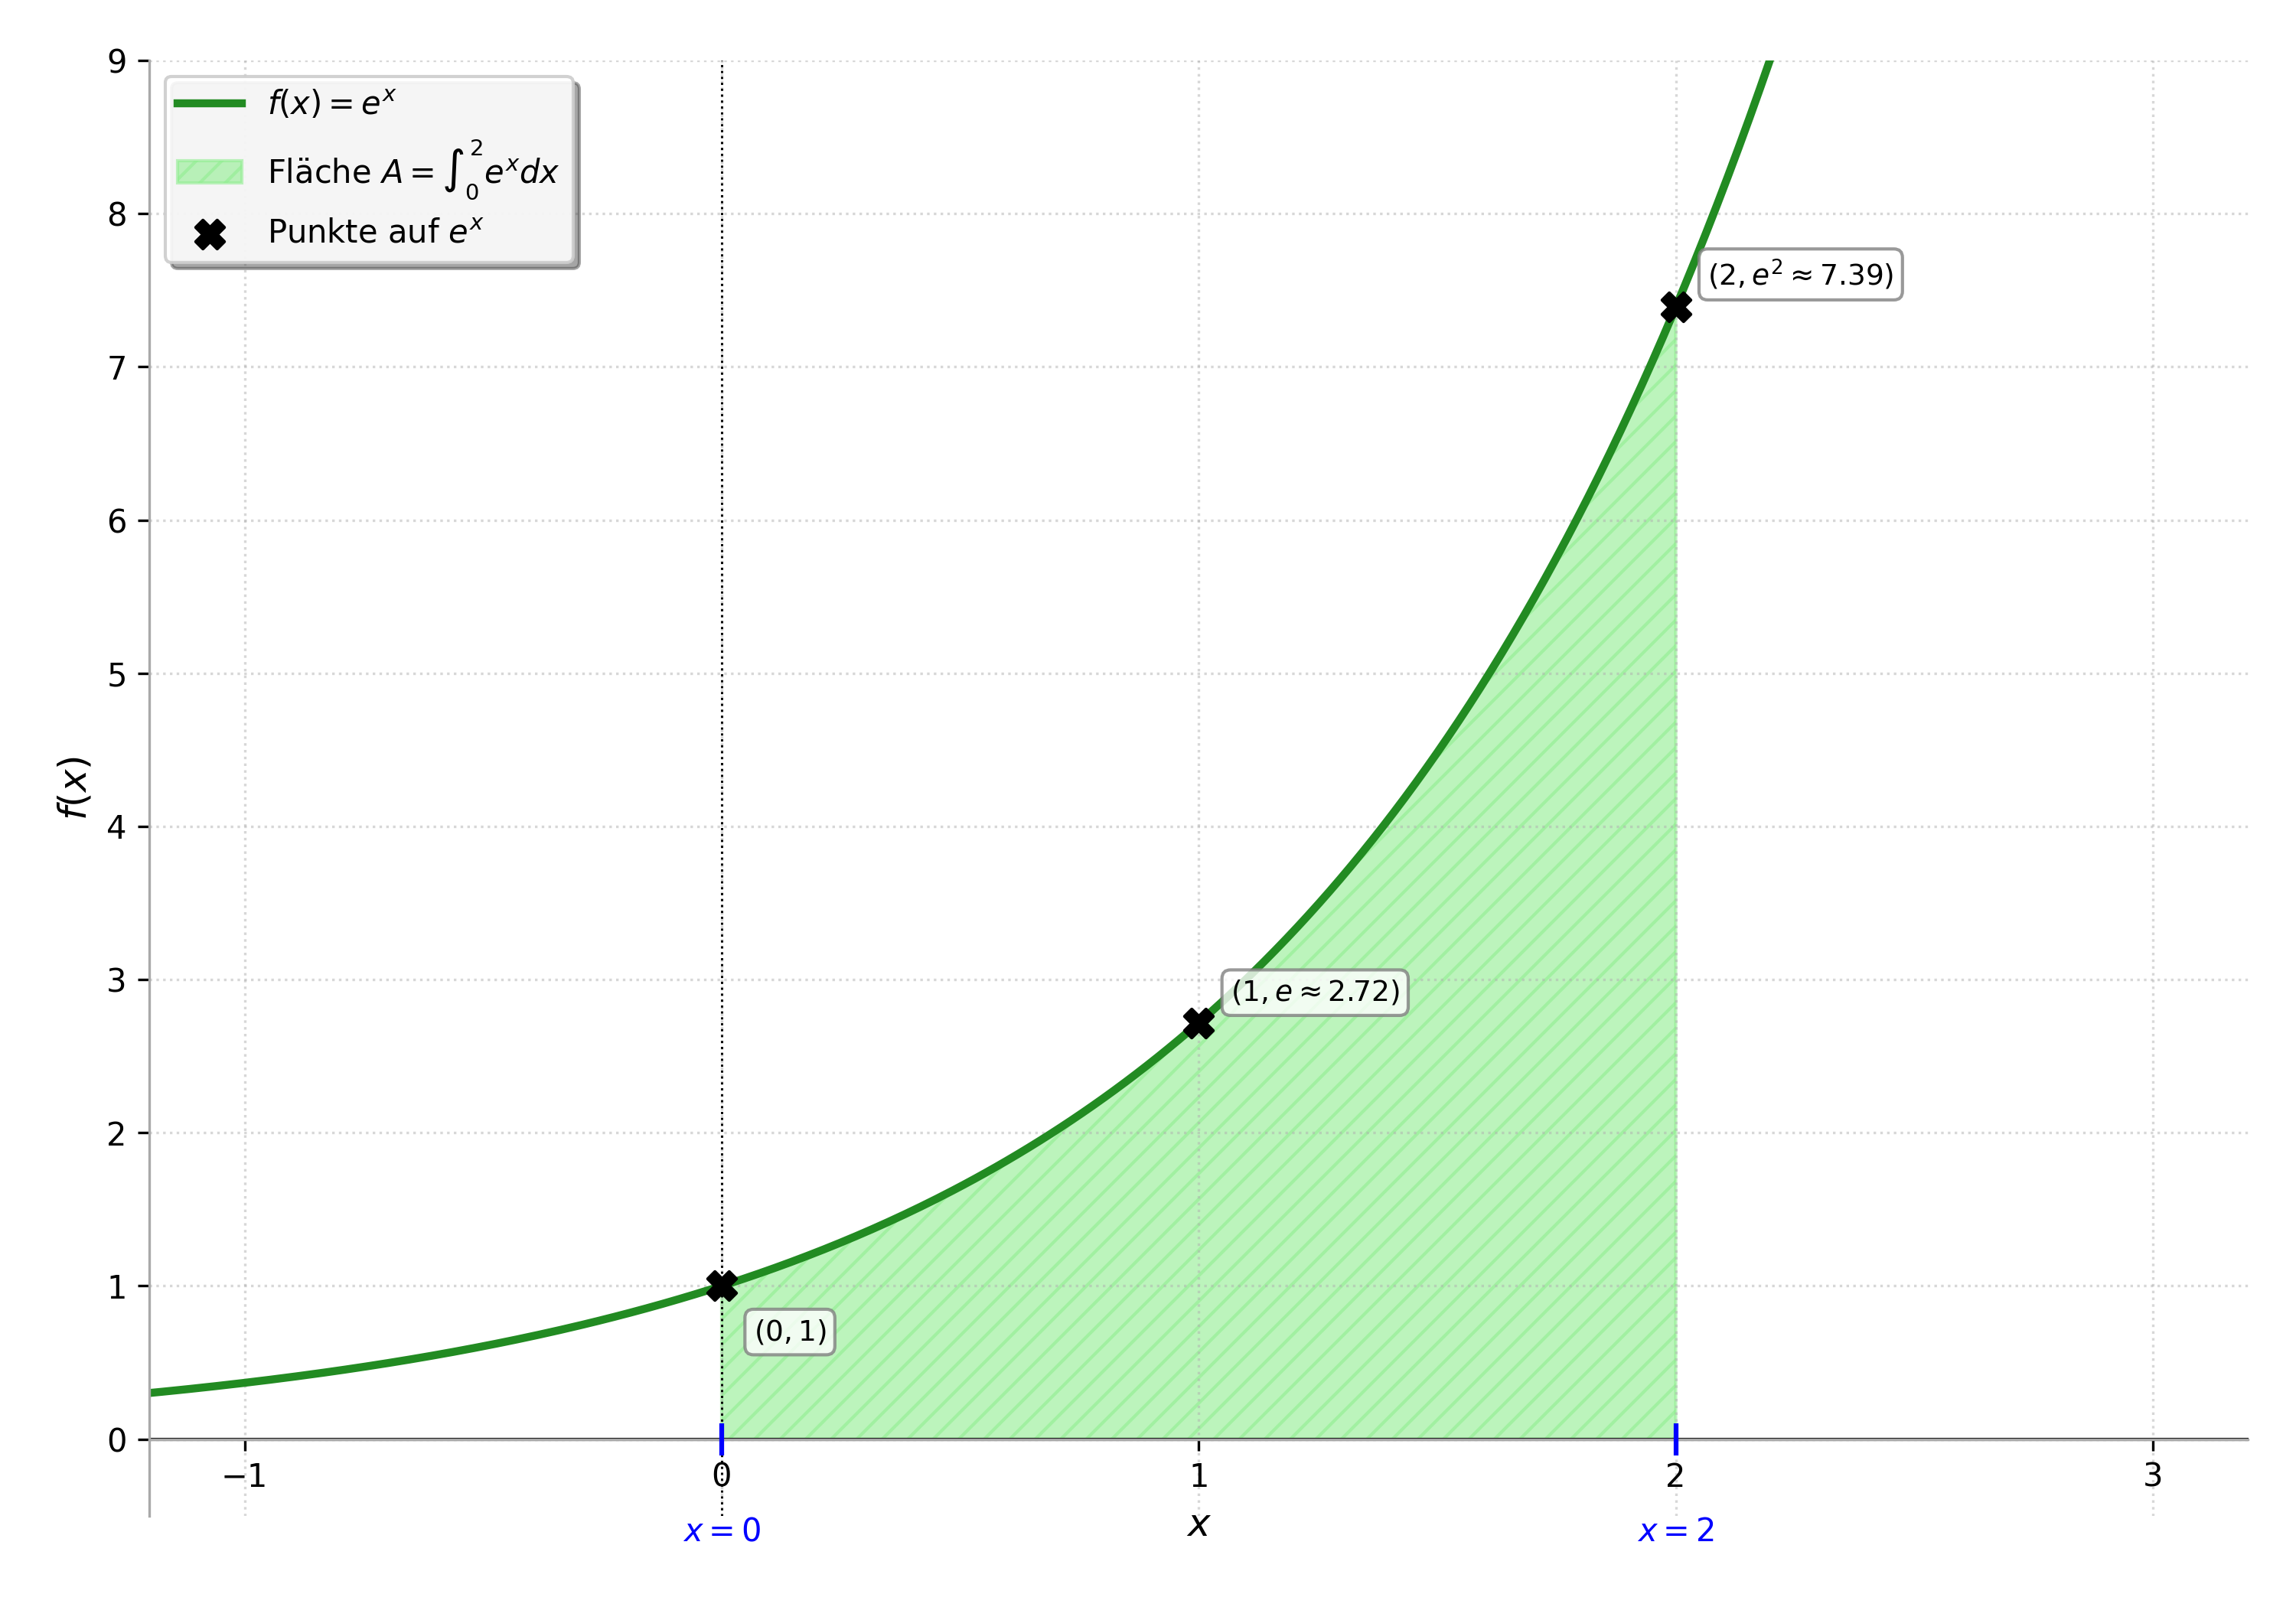
\includegraphics[width=0.8\textwidth]{grafiken/flaeche_ex_0_2.png}
    % --- Beschreibung der Skizze ---
    % Die Skizze zeigt den Graphen der Funktion f(x)=e^x.
    % Die x-Achse ist von etwa -1 bis 3 skaliert, die y-Achse von 0 bis etwa 8.
    % Der Graph steigt exponentiell an und geht durch (0|1) und (1|e) und (2|e^2).
    % Die Fläche unter dem Graphen zwischen x=0 (y-Achse) und x=2 ist markiert.
    \captionof{figure}{Fläche unter $f(x)=e^x$ im Intervall $[0,2]$.}
    \label{fig:flaeche_ex_0_2}
    \end{center}

    \item \textbf{Fläche unter $g(x) = 2e^{-0.5x}$ im Intervall $[0, 4]$:}
    Die Funktion $g(x)=2e^{-0.5x}$ ist im gesamten Intervall $[0,4]$ positiv. Der gesuchte Flächeninhalt $A_2$ ist daher gleich dem bestimmten Integral:
    $$ A_2 = \int_0^4 2e^{-0.5x} \,dx $$
    Eine Stammfunktion von $2e^{-0.5x}$ ist $G(x) = 2 \cdot \frac{1}{-0.5}e^{-0.5x} = 2 \cdot (-2)e^{-0.5x} = -4e^{-0.5x}$.
    \begin{align*}
    A_2 &= [-4e^{-0.5x}]_0^4 \\
        &= (-4e^{-0.5 \cdot 4}) - (-4e^{-0.5 \cdot 0}) \\
        &= (-4e^{-2}) - (-4e^0) \\
        &= -4e^{-2} - (-4 \cdot 1) \\
        &= 4 - 4e^{-2} = \mathbf{4 - \frac{4}{e^2}}
    \end{align*}
    Numerisch ist $A_2 \approx 4 - \frac{4}{(2.71828)^2} \approx 4 - \frac{4}{7.38906} \approx 4 - 0.54134 \approx 3.45866$.
    Der Flächeninhalt beträgt $4 - \frac{4}{e^2} \approx 3.459$ Flächeneinheiten.
    \begin{center}
    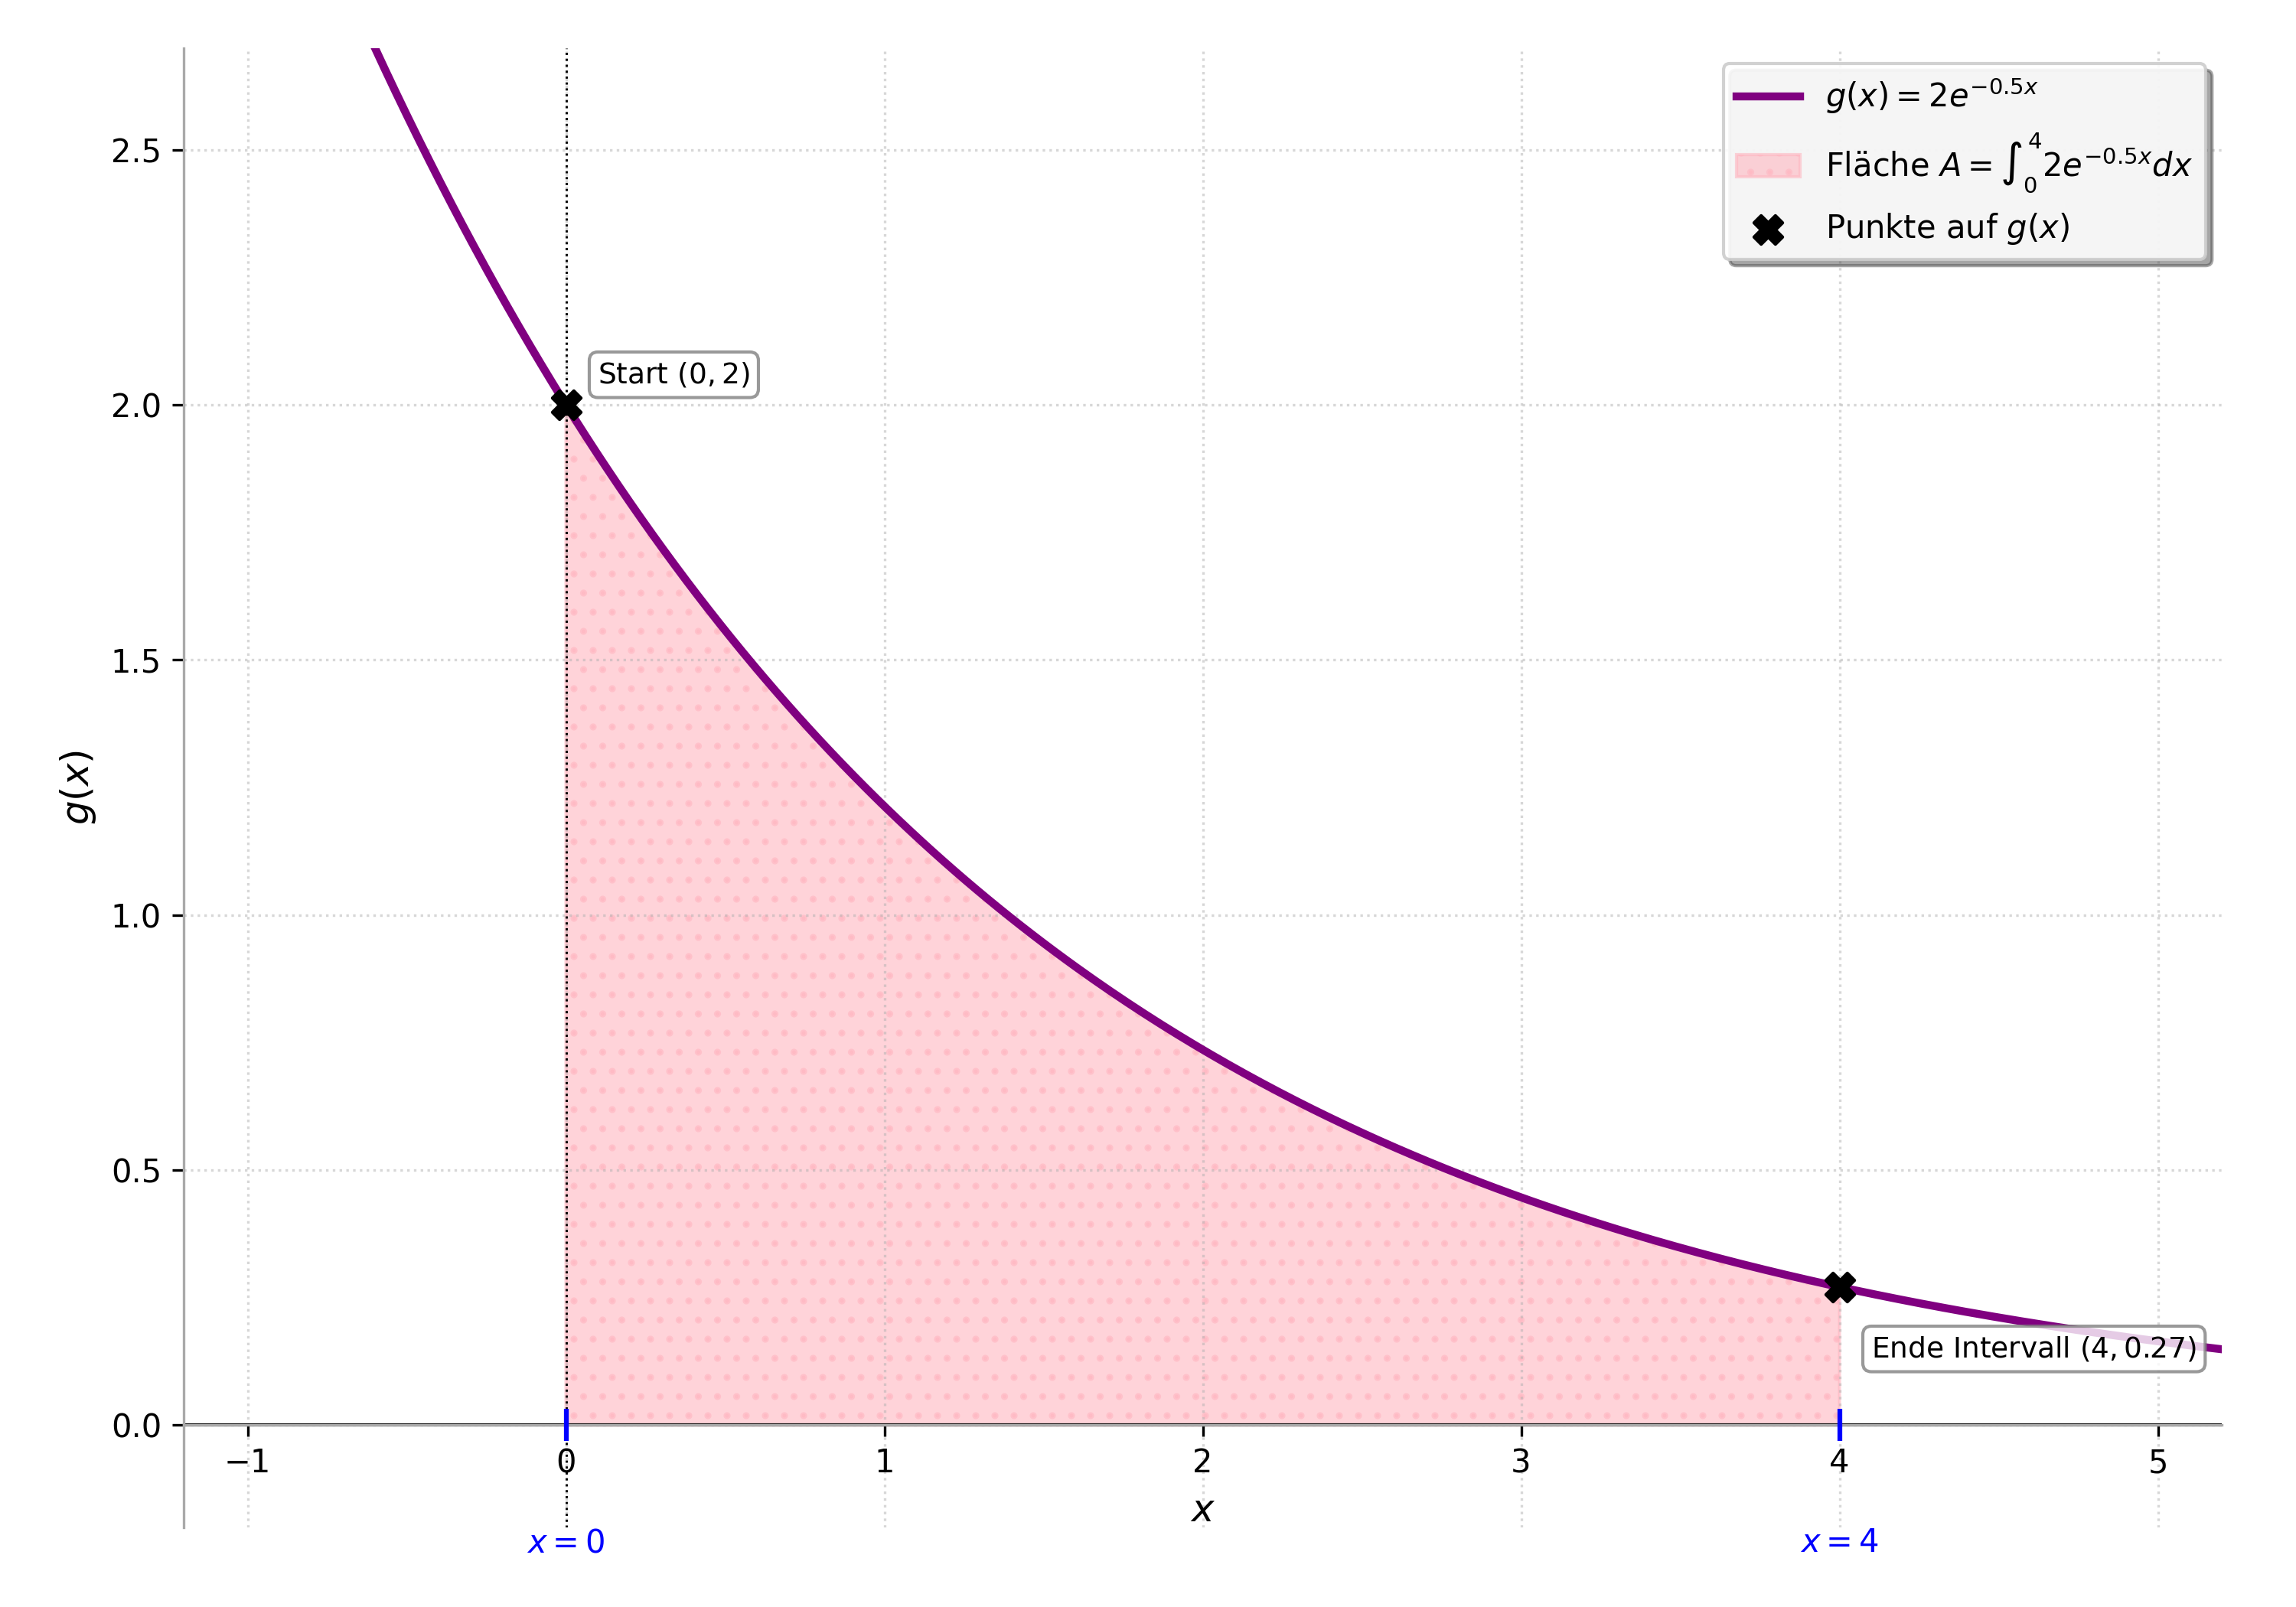
\includegraphics[width=0.8\textwidth]{grafiken/flaeche_2e_neg05x_0_4.png}
    % --- Beschreibung der Skizze ---
    % Die Skizze zeigt den Graphen der Funktion g(x)=2e^(-0.5x).
    % Die x-Achse ist von etwa -1 bis 5 skaliert, die y-Achse von 0 bis etwa 2.5.
    % Der Graph ist eine fallende Exponentialfunktion, die bei (0|2) beginnt und sich für x->unendlich der x-Achse nähert.
    % Die Fläche unter dem Graphen zwischen x=0 und x=4 ist markiert. Bei x=4 ist g(4) = 2e^-2 approx 0.27.
    \captionof{figure}{Fläche unter $g(x)=2e^{-0.5x}$ im Intervall $[0,4]$.}
    \label{fig:flaeche_2e_neg05x_0_4}
    \end{center}

    \item \textbf{Fläche zwischen $f(x) = e^x$ und $h(x) = ex + 1$:}
    \begin{itemize}
        \item \textbf{Zeige, dass sich die Graphen an der Stelle $x=0$ und $x=1$ schneiden.} \\
        Für $x=0$:
        $f(0) = e^0 = 1$.
        $h(0) = e \cdot 0 + 1 = 1$.
        Da $f(0)=h(0)=1$, schneiden sich die Graphen bei $x=0$.
        Für $x=1$:
        $f(1) = e^1 = e$.
        $h(1) = e \cdot 1 + 1 = e+1$.
        Da $f(1) = e$ und $h(1) = e+1$ und $e \neq e+1$, ist die Aussage, dass sich die Graphen auch bei $x=1$ schneiden, für die gegebene Funktion $h(x)=ex+1$ \textbf{nicht korrekt}.
        Wir fahren mit der Aufgabenstellung fort unter der Annahme, dass das Intervall $[0,1]$ für die Flächenberechnung relevant ist, auch wenn $x=1$ kein Schnittpunkt ist, oder dass eine andere Funktion $h(x)$ gemeint war, die $f(x)$ bei $x=1$ schneidet. Die Abbildung \ref{fig:flaeche_ex_gerade} im Aufgabentext suggeriert ein abgeschlossenes Flächenstück. Wenn wir die Funktionen wie gegeben verwenden, ist $x=0$ der einzige Schnittpunkt.

        \item \textbf{Bestimme, welche Funktion im Intervall $[0,1]$ oben bzw. unten liegt.}
        Wir vergleichen $f(x)=e^x$ und $h(x)=ex+1$ im Intervall $[0,1]$.
        Betrachten wir die Differenzfunktion $d(x) = h(x) - f(x) = ex+1 - e^x$.
        $d(0) = e(0)+1 - e^0 = 1-1 = 0$.
        $d(1) = e(1)+1 - e^1 = e+1-e = 1$.
        Um das Verhalten dazwischen zu prüfen, betrachten wir $d'(x) = e - e^x$.
        $d'(x)=0 \Rightarrow e^x=e \Rightarrow x=1$.
        $d''(x) = -e^x$. $d''(1) = -e < 0$. Also hat $d(x)$ ein Maximum bei $x=1$.
        Da $d(0)=0$ und $d(1)=1$ (Maximum), und $d(x)$ stetig ist, muss $d(x) \ge 0$ für $x \in [0,1]$ gelten.
        Somit liegt $\mathbf{h(x) = ex+1}$ im Intervall $[0,1]$ \textbf{oberhalb oder gleich} $\mathbf{f(x) = e^x}$.

        \item \textbf{Berechne den Inhalt der eingeschlossenen Fläche.}
        Da $h(x) \ge f(x)$ im Intervall $[0,1]$ und $x=0$ der einzige Schnittpunkt in diesem Bereich ist (und $x=1$ die rechte Grenze des Intervalls, aber kein Schnittpunkt mit $f(x)$ ist, wie oben gezeigt), berechnen wir die Fläche $A_3 = \int_0^1 (h(x)-f(x)) \,dx$.
        \begin{align*}
        A_3 &= \int_0^1 (ex+1 - e^x) \,dx \\
            &= \left[ e\frac{x^2}{2} + x - e^x \right]_0^1 \\
            &= \left( e\frac{1^2}{2} + 1 - e^1 \right) - \left( e\frac{0^2}{2} + 0 - e^0 \right) \\
            &= \left( \frac{e}{2} + 1 - e \right) - (0 + 0 - 1) \\
            &= \left( 1 - \frac{e}{2} \right) - (-1) \\
            &= 1 - \frac{e}{2} + 1 \\
            &= \mathbf{2 - \frac{e}{2}}
        \end{align*}
        Numerisch ist $A_3 \approx 2 - \frac{2.71828}{2} \approx 2 - 1.35914 = 0.64086$.
        Der Flächeninhalt beträgt $2 - \frac{e}{2} \approx 0.641$ Flächeneinheiten.
    \end{itemize}
\end{enumerate}

\end{loesungsumgebung}



\begin{aufgabenumgebung}{Anwendung: Medikamentenabbau im Körper}
Die Konzentration eines Medikaments im Blut eines Patienten (in mg/Liter) kann nach der Einnahme durch die Funktion $K(t) = 10 \cdot t \cdot e^{-0.2t}$ beschrieben werden, wobei $t$ die Zeit in Stunden nach der Einnahme ist ($t \ge 0$).
\begin{enumerate}
    \item Zu welchem Zeitpunkt ist die Konzentration des Medikaments maximal? Wie hoch ist diese maximale Konzentration? (Nutze die Differentialrechnung).
    \item Die 'Gesamtwirkung' eines Medikaments über einen bestimmten Zeitraum kann manchmal durch das Integral der Konzentrationsfunktion über diesen Zeitraum angenähert werden (dies ist eine Vereinfachung, aber das Integral gibt eine Art 'kumulierte Dosis' an).
        Berechne $\int_0^{10} K(t) \,dt$. (Tipp: Partielle Integration ist hier notwendig! Wähle $u'(t)=e^{-0.2t}$ und $v(t)=10t$).
        Was könnte dieser Wert im Kontext bedeuten?
    \item (Für Experten): Was ist $\lim_{t \to \infty} K(t)$? Was bedeutet das für die Konzentration des Medikaments nach sehr langer Zeit?
\end{enumerate}
\end{aufgabenumgebung}


\begin{loesungsumgebung}[loes:anwendung-medikamentenabbau]{Anwendung: Medikamentenabbau im Körper}
Die Konzentration des Medikaments wird durch $K(t) = 10t \cdot e^{-0.2t}$ beschrieben ($t \ge 0$).

\begin{enumerate}[label=(\alph*)]
    \item \textbf{Zu welchem Zeitpunkt ist die Konzentration des Medikaments maximal? Wie hoch ist diese maximale Konzentration?}
    Um das Maximum zu finden, bilden wir die erste Ableitung $K'(t)$ und setzen sie gleich Null.
    $K(t) = 10t \cdot e^{-0.2t}$. Wir verwenden die Produktregel ($u=10t, v=e^{-0.2t}$):
    $u'(t) = 10$.
    $v'(t) = e^{-0.2t} \cdot (-0.2) = -0.2e^{-0.2t}$ (Kettenregel).
    \begin{align*} K'(t) &= 10 \cdot e^{-0.2t} + 10t \cdot (-0.2e^{-0.2t}) \\ &= 10e^{-0.2t} - 2te^{-0.2t} \\ &= e^{-0.2t}(10 - 2t) \end{align*}
    Setze $K'(t)=0$:
    $e^{-0.2t}(10 - 2t) = 0$.
    Da $e^{-0.2t} > 0$ für alle $t$, muss $10 - 2t = 0$ sein.
    $10 = 2t \Rightarrow t = 5$.
    Die kritische Stelle ist $t_{max} = 5$ Stunden.
    Um zu überprüfen, ob es sich um ein Maximum handelt, bilden wir die zweite Ableitung $K''(t)$:
    $K'(t) = (10 - 2t)e^{-0.2t}$. Mit Produktregel ($u_2=10-2t, v_2=e^{-0.2t}$):
    $u_2'(t) = -2$.
    $v_2'(t) = -0.2e^{-0.2t}$.
    \begin{align*} K''(t) &= -2 \cdot e^{-0.2t} + (10 - 2t) \cdot (-0.2e^{-0.2t}) \\ &= e^{-0.2t}[-2 - 0.2(10 - 2t)] \\ &= e^{-0.2t}[-2 - 2 + 0.4t] \\ &= e^{-0.2t}(0.4t - 4) \end{align*}
    Setze $t=5$ in $K''(t)$ ein:
    $K''(5) = e^{-0.2 \cdot 5}(0.4 \cdot 5 - 4) = e^{-1}(2 - 4) = e^{-1}(-2) = -\frac{2}{e}$.
    Da $K''(5) < 0$, liegt bei $t=5$ Stunden ein lokales Maximum vor.
    Die maximale Konzentration ist:
    $K(5) = 10 \cdot 5 \cdot e^{-0.2 \cdot 5} = 50e^{-1} = \frac{50}{e}$.
    $K(5) \approx \frac{50}{2.71828} \approx 18.394$.
    Die Konzentration ist \textbf{nach 5 Stunden maximal} und beträgt dann $\mathbf{\frac{50}{e} \approx 18.394}$ mg/Liter.

    \item \textbf{Berechne $\int_0^{10} K(t) \,dt$.}
    Wir verwenden partielle Integration für $\int 10t e^{-0.2t} \,dt$.
    Sei $u(t) = 10t \Rightarrow u'(t) = 10$.
    Sei $v'(t) = e^{-0.2t} \Rightarrow v(t) = \int e^{-0.2t} \,dt = \frac{1}{-0.2}e^{-0.2t} = -5e^{-0.2t}$.
    \begin{align*} \int 10t e^{-0.2t} \,dt &= 10t(-5e^{-0.2t}) - \int 10(-5e^{-0.2t}) \,dt \\ &= -50te^{-0.2t} - \int -50e^{-0.2t} \,dt \\ &= -50te^{-0.2t} + 50 \int e^{-0.2t} \,dt \\ &= -50te^{-0.2t} + 50 \left(\frac{1}{-0.2}e^{-0.2t}\right) + C \\ &= -50te^{-0.2t} - 250e^{-0.2t} + C \\ &= -50e^{-0.2t}(t+5) + C \end{align*}
    Nun das bestimmte Integral von $0$ bis $10$:
    \begin{align*} \int_0^{10} 10t e^{-0.2t} \,dt &= [-50e^{-0.2t}(t+5)]_0^{10} \\ &= \left(-50e^{-0.2 \cdot 10}(10+5)\right) - \left(-50e^{-0.2 \cdot 0}(0+5)\right) \\ &= \left(-50e^{-2}(15)\right) - \left(-50e^0(5)\right) \\ &= -750e^{-2} - (-250 \cdot 1) \\ &= 250 - 750e^{-2} = \mathbf{250 - \frac{750}{e^2}} \end{align*}
    Numerischer Wert: $250 - \frac{750}{(2.71828)^2} \approx 250 - \frac{750}{7.38906} \approx 250 - 101.501 \approx 148.499$.
    \textit{Bedeutung:} Der Wert $\mathbf{250 - \frac{750}{e^2} \approx 148.5}$ (mg/Liter)$\cdot$Stunden stellt die kumulierte Medikamentenexposition des Patienten über die ersten 10 Stunden dar. Es ist ein Maß für die Gesamtmenge des Medikaments, der der Körper in diesem Zeitraum ausgesetzt war (Fläche unter der Konzentrationskurve).

    \item \textbf{(Für Experten): Was ist $\lim_{t \to \infty} K(t)$?}
    $$ K(t) = 10t e^{-0.2t} = \frac{10t}{e^{0.2t}} $$
    Für $t \to \infty$ wächst der Nenner $e^{0.2t}$ schneller als der Zähler $10t$. Mit der Regel von L'Hôpital:
    $$ \lim_{t \to \infty} \frac{10t}{e^{0.2t}} \stackrel{L'H}{=} \lim_{t \to \infty} \frac{\frac{d}{dt}(10t)}{\frac{d}{dt}(e^{0.2t})} = \lim_{t \to \infty} \frac{10}{0.2e^{0.2t}} $$
    Da $e^{0.2t} \to \infty$ für $t \to \infty$, ist der Grenzwert:
    $$ \lim_{t \to \infty} \frac{10}{0.2e^{0.2t}} = \frac{10}{\infty} = \mathbf{0} $$
    \textit{Bedeutung:} Für sehr große Zeiten ($t \to \infty$) nähert sich die Konzentration des Medikaments im Blut Null an. Das bedeutet, dass das Medikament im Laufe der Zeit vollständig aus dem Körper eliminiert oder abgebaut wird, was biologisch erwartet wird.
\end{enumerate}

\end{loesungsumgebung}



\begin{aufgabenumgebung}{Uneigentliches Integral – Fläche bis ins Unendliche?}
Wir betrachten die Funktion $f(x) = e^{-x}$ für $x \ge 0$.
\begin{enumerate}
    \item Skizziere den Graphen von $f(x)$.
    \item Berechne den Flächeninhalt $A_b = \int_0^b e^{-x} \,dx$ für eine beliebige obere Grenze $b > 0$.
    \item Was passiert mit diesem Flächeninhalt $A_b$, wenn $b$ unendlich groß wird? Berechne also den Grenzwert $\lim_{b \to \infty} A_b$.
    \item Kann eine Fläche, die sich ins Unendliche erstreckt, einen endlichen Inhalt haben? Diskutiere dein Ergebnis aus c).
\end{enumerate}
\end{aufgabenumgebung}

\begin{loesungsumgebung}[loes:uneigentliches-integral-flaeche]{Uneigentliches Integral – Fläche bis ins Unendliche?}
Wir betrachten die Funktion $f(x) = e^{-x}$ für $x \ge 0$.

\begin{enumerate}[label=(\alph*)]
    \item \textbf{Skizziere den Graphen von $f(x)$.}
    Die Funktion $f(x)=e^{-x}$ ist eine monoton fallende Exponentialfunktion.
    \begin{itemize}
        \item Bei $x=0$ ist $f(0)=e^0=1$. Der Graph startet im Punkt $(0|1)$.
        \item Für $x > 0$ ist $f(x) > 0$. Der Graph verläuft vollständig oberhalb der x-Achse.
        \item Für $x \to \infty$ nähert sich $f(x)=e^{-x} = \frac{1}{e^x}$ dem Wert $0$. Die x-Achse ($y=0$) ist eine horizontale Asymptote.
    \end{itemize}
    \begin{center}
    % \includegraphics[width=0.8\textwidth]{grafiken/uneigentliches_integral_ex.png}
    % --- Beschreibung der Skizze ---
    % Die Skizze zeigt ein Koordinatensystem mit x- und y-Achse.
    % Der Graph der Funktion f(x) = e^(-x) ist für x >= 0 eingezeichnet.
    % Er startet bei (0|1) auf der y-Achse.
    % Er fällt exponentiell ab und nähert sich für x -> unendlich der x-Achse (horizontale Asymptote y=0).
    % Die Fläche zwischen dem Graphen, der x-Achse, der y-Achse (x=0) und einer vertikalen Linie bei x=b ist schattiert.
    % Eine Andeutung, dass b gegen unendlich geht, kann durch einen Pfeil oder die Beschriftung der schattierten Fläche als A_unendlich erfolgen.
    \captionof{figure}{Graph der Funktion $f(x)=e^{-x}$ für $x \ge 0$.}
    \label{fig:uneigentliches_integral_ex}
    \end{center}

    \item \textbf{Berechne den Flächeninhalt $A_b = \int_0^b e^{-x} \,dx$ für eine beliebige obere Grenze $b > 0$.}
    Eine Stammfunktion von $f(x)=e^{-x}$ ist $F(x) = -e^{-x}$.
    \begin{align*} A_b &= \int_0^b e^{-x} \,dx \\ &= [-e^{-x}]_0^b \\ &= (-e^{-b}) - (-e^{-0}) \\ &= -e^{-b} - (-1) \\ &= \mathbf{1 - e^{-b}} \quad \text{oder} \quad \mathbf{1 - \frac{1}{e^b}} \end{align*}

    \item \textbf{Was passiert mit diesem Flächeninhalt $A_b$, wenn $b$ unendlich groß wird? Berechne also den Grenzwert $\lim_{b \to \infty} A_b$.}
    Wir berechnen den Grenzwert des Ergebnisses aus Teil (b) für $b \to \infty$:
    $$ \lim_{b \to \infty} A_b = \lim_{b \to \infty} \left(1 - e^{-b}\right) = \lim_{b \to \infty} \left(1 - \frac{1}{e^b}\right) $$
    Wenn $b \to \infty$, dann $e^b \to \infty$, und somit $\frac{1}{e^b} \to 0$.
    Also:
    $$ \lim_{b \to \infty} A_b = 1 - 0 = \mathbf{1} $$
    Dieser Grenzwert ist der Wert des uneigentlichen Integrals $\int_0^\infty e^{-x} \,dx$.

    \item \textbf{Kann eine Fläche, die sich ins Unendliche erstreckt, einen endlichen Inhalt haben? Diskutiere dein Ergebnis aus c).}
    \textbf{Ja}, eine Fläche, die sich ins Unendliche erstreckt, kann einen endlichen Inhalt haben. Das Ergebnis aus Teil (c), $\int_0^\infty e^{-x} \,dx = 1$, ist ein Beispiel dafür.
    \textit{Diskussion:}
    Obwohl sich der Integrationsbereich $[0, \infty)$ unendlich weit entlang der x-Achse ausdehnt, nähert sich die Funktion $f(x)=e^{-x}$ für $x \to \infty$ sehr schnell der x-Achse an (d.h., die 'Höhe' der Fläche wird sehr klein). Der Beitrag der Fläche für immer größere $x$-Werte wird so gering, dass die Summe aller Flächenbeiträge (das Integral) gegen einen endlichen Wert konvergiert.
    Man kann sich das so vorstellen, dass der 'Schwanz' der Fläche so schnell dünn wird, dass sein Gesamtinhalt begrenzt ist. Nicht jede Funktion, die sich ins Unendliche erstreckt, hat eine endliche Fläche (z.B. $\int_1^\infty \frac{1}{x} \,dx$ divergiert), aber für Funktionen, die schnell genug gegen Null gehen, wie $e^{-x}$, ist dies möglich. Das Konzept der Konvergenz von Reihen und uneigentlichen Integralen beschäftigt sich genau mit solchen Phänomenen.
\end{enumerate}

\end{loesungsumgebung}


\begin{aufgabenumgebung}{Exponentialfunktionen – Übergreifende und anspruchsvolle Aufgaben}
Die folgenden Aufgaben sollen dein Verständnis für Exponentialfunktionen, ihre Ableitungen, Stammfunktionen und Anwendungen umfassend prüfen. Versuche, die Aufgaben sorgfältig und schrittweise zu lösen.
\begin{enumerate}
    \item \textbf{Kurvendiskussion einer e-Funktion mit Polynomfaktor:}
        Führe eine vollständige Kurvendiskussion für die Funktion $f(x) = (4-x^2)e^{-0.5x}$ durch. Untersuche dabei insbesondere:
        \begin{itemize}
            \item Definitionsbereich und Symmetrie.
            \item Verhalten im Unendlichen und Asymptoten. (Tipp: $\lim_{x\to\infty} x^n e^{-kx} = 0$ für $k>0$).
            \item Nullstellen.
            \item Extrempunkte (Lage und Art).
            \item Wendepunkte (Lage und Krümmungsverhalten).
            \item Skizziere den Graphen von $f(x)$.
        \end{itemize}

    \item \textbf{Optimierung: Maximale Konzentration eines Medikaments}
        Die Konzentration $K(t)$ eines Medikaments im Blut eines Patienten (in mg/l) zum Zeitpunkt $t$ (in Stunden nach Einnahme) wird durch die Funktion $K(t) = 20t \cdot e^{-0.25t}$ für $t \ge 0$ beschrieben.
        \begin{itemize}
            \item Zu welchem Zeitpunkt $t_{max}$ erreicht die Konzentration des Medikaments ihr Maximum?
            \item Wie hoch ist diese maximale Konzentration?
            \item Bestimme die Funktion $K'(t)$, die die Änderungsrate der Konzentration angibt. Wann nimmt die Konzentration am stärksten zu? (Suche nach dem Maximum von $K'(t)$, also einem Wendepunkt von $K(t)$ mit bestimmten Eigenschaften).
        \end{itemize}

    \item \textbf{Flächenberechnung und uneigentliches Integral:}
        Gegeben ist die Funktion $f(x) = (x+1)e^{-x}$.
        \begin{itemize}
            \item Bestimme die Stammfunktion $F(x)$ von $f(x)$ mithilfe partieller Integration.
            \item Berechne den Inhalt der Fläche, die der Graph von $f(x)$ mit der x-Achse und der y-Achse im ersten Quadranten einschließt. (Finde dazu die Nullstelle von $f(x)$ für $x \ge 0$).
            \item (Für Experten): Untersuche, ob die Fläche, die der Graph von $f(x)$ mit der x-Achse für $x \ge 0$ einschließt, einen endlichen Inhalt hat. Berechne dazu das uneigentliche Integral $\int_0^\infty (x+1)e^{-x} \,dx = \lim_{b \to \infty} \int_0^b (x+1)e^{-x} \,dx$.
        \end{itemize}

    \item \textbf{Rekonstruktion einer Exponentialfunktion und Tangente:}
        Eine Funktion $f$ ist gegeben durch $f(x) = (ax+b)e^{-x}$. Der Graph von $f$ hat im Punkt $P(0|2)$ eine Tangente, die parallel zur Geraden $y=3x-5$ ist.
        \begin{itemize}
            \item Bestimme die Werte der Parameter $a$ und $b$.
            \item Bestimme die Gleichung der Tangente an den Graphen von $f$ im Punkt $P(0|2)$.
            \item Untersuche die Funktion $f(x)$ mit den gefundenen Parametern auf Nullstellen und Extrempunkte.
        \end{itemize}

    \item \textbf{Schar von Exponentialfunktionen (Schwer):}
        Gegeben ist die Funktionenschar $f_k(x) = x^2 e^{kx}$ mit dem Scharparameter $k \in \mathbb{R}$, $k \neq 0$.
        \begin{itemize}
            \item Bestimme die Nullstellen von $f_k(x)$.
            \item Bestimme die erste Ableitung $f_k'(x)$. Für welche Werte von $x$ (in Abhängigkeit von $k$) ist $f_k'(x)=0$?
            \item Untersuche die Art der Extremstellen in Abhängigkeit von $k$. (Tipp: Betrachte die Fälle $k>0$ und $k<0$ getrennt für das Verhalten der zweiten Ableitung oder den Vorzeichenwechsel der ersten Ableitung).
            \item Gibt es Werte für $k$, sodass die Funktion keine Extrempunkte besitzt?
        \end{itemize}
\end{enumerate}
\end{aufgabenumgebung}

\begin{loesungsumgebung}[loes:A:DiffUebergreifend]{Übergreifende Übungsaufgaben}

\begin{enumerate}
    \item \textbf{Kurvendiskussion einer e-Funktion mit Polynomfaktor: $f(x) = (4-x^2)e^{-0.5x}$}
    \begin{itemize}
        \item \textbf{Definitionsbereich und Symmetrie:}
        $D_f = \mathbb{R}$, da sowohl der Polynomfaktor als auch die e-Funktion für alle $x \in \mathbb{R}$ definiert sind.
        $f(-x) = (4-(-x)^2)e^{-0.5(-x)} = (4-x^2)e^{0.5x}$.
        Da $f(-x) \neq f(x)$ und $f(-x) \neq -f(x)$, liegt keine einfache Achsen- oder Punktsymmetrie zum Ursprung vor.

        \item \textbf{Verhalten im Unendlichen und Asymptoten:}
        Für $x \to \infty$: $f(x) = \frac{4-x^2}{e^{0.5x}}$. Da die e-Funktion im Nenner schneller wächst als jedes Polynom im Zähler (vgl. Regel von L'Hôpital, zweimal angewendet $\lim \frac{-2x}{0.5e^{0.5x}} = \lim \frac{-2}{0.25e^{0.5x}} = 0$), gilt $\lim_{x\to\infty} f(x) = 0$.
        Somit ist $\mathbf{y=0}$ eine horizontale Asymptote für $x \to \infty$.
        Für $x \to -\infty$: Sei $u=-x$, dann $u \to \infty$. $f(x) = (4-u^2)e^{0.5u}$.
        $\lim_{u\to\infty} (4-u^2)e^{0.5u} = (-\infty) \cdot (\infty) = -\infty$. Also $\lim_{x\to-\infty} f(x) = -\infty$.

        \item \textbf{Nullstellen:}
        $f(x)=0 \Rightarrow (4-x^2)e^{-0.5x}=0$. Da $e^{-0.5x} > 0$ immer, muss $4-x^2=0 \Rightarrow x^2=4 \Rightarrow x=\pm 2$.
        Nullstellen: $\mathbf{N_1(-2|0)}$ und $\mathbf{N_2(2|0)}$.
        Y-Achsenabschnitt: $f(0)=(4-0)e^0 = 4 \cdot 1 = 4$. $\mathbf{P_y(0|4)}$.

        \item \textbf{Extrempunkte (Lage und Art):}
        $f'(x) = (-2x)e^{-0.5x} + (4-x^2)(-0.5e^{-0.5x}) = e^{-0.5x}[-2x - 0.5(4-x^2)]$
        $f'(x) = e^{-0.5x}[-2x - 2 + 0.5x^2] = \frac{1}{2}e^{-0.5x}(x^2 - 4x - 4)$.
        $f'(x)=0 \Rightarrow x^2 - 4x - 4 = 0$.
        $x_{1,2} = \frac{4 \pm \sqrt{16-4(1)(-4)}}{2} = \frac{4 \pm \sqrt{32}}{2} = \frac{4 \pm 4\sqrt{2}}{2} = 2 \pm 2\sqrt{2}$.
        $x_{E1} = 2 - 2\sqrt{2} \approx -0.828$, $x_{E2} = 2 + 2\sqrt{2} \approx 4.828$.
        $f''(x) = \frac{d}{dx}\left(\frac{1}{2}e^{-0.5x}(x^2 - 4x - 4)\right)$
        $f''(x) = \frac{1}{2}[-0.5e^{-0.5x}(x^2-4x-4) + e^{-0.5x}(2x-4)]$
        $f''(x) = \frac{1}{2}e^{-0.5x}[-0.5x^2+2x+2 + 2x-4] = \frac{1}{2}e^{-0.5x}(-0.5x^2+4x-2) = \frac{1}{4}e^{-0.5x}(-x^2+8x-4)$.
        $f''(2-2\sqrt{2}) = \frac{1}{4}e^{-0.5(2-2\sqrt{2})} \underbrace{(-(2-2\sqrt{2})^2+8(2-2\sqrt{2})-4)}_{ \approx - (0.686) + 8(-0.828) - 4 = -0.686 -6.624 -4 < 0 \text{ (genauer Wert über } x^2-4x-4=0 \text{ für } f' \text{ nutzen)}}$.
        Für $x_E = 2 \pm 2\sqrt{2}$ ist $x_E^2-4x_E-4=0$. Die Klammer in $f''(x_E)$ ist $\frac{1}{2}e^{-0.5x_E}[ (2x_E-4)]$.
        Für $x_{E1}=2-2\sqrt{2} \approx -0.828$: $2x_{E1}-4 = 4-4\sqrt{2}-4 = -4\sqrt{2} < 0$. Also $f''(x_{E1}) = \frac{1}{2}e^{-0.5x_{E1}}(-4\sqrt{2}) < 0 \implies \mathbf{HP}$.
        $f(2-2\sqrt{2}) = (4-(2-2\sqrt{2})^2)e^{-0.5(2-2\sqrt{2})} = (4-(4-8\sqrt{2}+8))e^{\sqrt{2}-1} = (4-12+8\sqrt{2})e^{\sqrt{2}-1} = (8\sqrt{2}-8)e^{\sqrt{2}-1} \approx 4.54$.
        $HP(2-2\sqrt{2} | (8\sqrt{2}-8)e^{\sqrt{2}-1})$.
        Für $x_{E2}=2+2\sqrt{2} \approx 4.828$: $2x_{E2}-4 = 4+4\sqrt{2}-4 = 4\sqrt{2} > 0$. Also $f''(x_{E2}) = \frac{1}{2}e^{-0.5x_{E2}}(4\sqrt{2}) > 0 \implies \mathbf{TP}$.
        $f(2+2\sqrt{2}) = (4-(2+2\sqrt{2})^2)e^{-0.5(2+2\sqrt{2})} = (4-(4+8\sqrt{2}+8))e^{-1-2\sqrt{2}} = (-8-8\sqrt{2})e^{-1-2\sqrt{2}} \approx -0.21$.
        $TP(2+2\sqrt{2} | (-8-8\sqrt{2})e^{-1-2\sqrt{2}})$.

        \item \textbf{Wendepunkte und Krümmungsverhalten:}
        $f''(x) = \frac{1}{4}e^{-0.5x}(-x^2+8x-4)$. $f''(x)=0 \Rightarrow -x^2+8x-4=0 \Rightarrow x^2-8x+4=0$.
        $x_{W1,2} = \frac{8 \pm \sqrt{64-16}}{2} = \frac{8 \pm \sqrt{48}}{2} = \frac{8 \pm 4\sqrt{3}}{2} = 4 \pm 2\sqrt{3}$.
        $x_{W1} = 4-2\sqrt{3} \approx 0.536$, $x_{W2} = 4+2\sqrt{3} \approx 7.464$.
        Da $-x^2+8x-4$ eine nach unten geöffnete Parabel ist:
        Linksgekrümmt ($f''(x)>0$) für $4-2\sqrt{3} < x < 4+2\sqrt{3}$.
        Rechtsgekrümmt ($f''(x)<0$) für $x < 4-2\sqrt{3}$ und $x > 4+2\sqrt{3}$.
        Wendepunkte bei $x_{W1}$ und $x_{W2}$.
        $WP_1(4-2\sqrt{3} | f(4-2\sqrt{3}))$, $WP_2(4+2\sqrt{3} | f(4+2\sqrt{3}))$.

        \item \textbf{Skizze des Graphen:}
        Der Graph von $f(x)$ startet für $x \to -\infty$ bei $f(x) \to -\infty$. Er hat Nullstellen bei $x=\pm 2$. Der y-Achsenabschnitt ist $P_y(0|4)$. Es gibt einen Hochpunkt bei $x \approx -0.828$ ($y \approx 4.54$) und einen Tiefpunkt bei $x \approx 4.828$ ($y \approx -0.21$). Für $x \to \infty$ nähert sich der Graph der Asymptote $y=0$. Wendepunkte liegen bei $x \approx 0.536$ und $x \approx 7.464$.
    \end{itemize}

    \item \textbf{Optimierung: Maximale Konzentration eines Medikaments} $K(t) = 20t e^{-0.25t}$ für $t \ge 0$.
    \begin{itemize}
        \item \textbf{Zeitpunkt $t_{max}$ der maximalen Konzentration:}
        $K'(t) = 20e^{-0.25t} + 20t(-0.25e^{-0.25t}) = 20e^{-0.25t}(1-0.25t)$.
        $K'(t)=0 \Rightarrow 1-0.25t=0 \Rightarrow 0.25t=1 \Rightarrow t_{max}=4$ Stunden.
        \item \textbf{Maximale Konzentration:}
        $K(4) = 20(4)e^{-0.25(4)} = 80e^{-1} = \frac{80}{e} \approx 29.43\,$mg/l.
        Zur Überprüfung: $K''(t) = 20(-0.25)e^{-0.25t}(1-0.25t) + 20e^{-0.25t}(-0.25) = -5e^{-0.25t}(1-0.25t+1) = -5e^{-0.25t}(2-0.25t)$.
        $K''(4) = -5e^{-1}(2-1) = -5e^{-1} < 0 \implies$ Maximum.
        \item \textbf{Änderungsrate $K'(t)$. Wann Zunahme am stärksten?}
        Die Zunahme ist am stärksten, wenn $K'(t)$ maximal ist, d.h. $(K'(t))'=K''(t)=0$.
        $K''(t) = -5e^{-0.25t}(2-0.25t)=0 \Rightarrow 2-0.25t=0 \Rightarrow 0.25t=2 \Rightarrow t_W=8$ Stunden.
        $(K'(t))''' = K'''(t) = -5(-0.25)e^{-0.25t}(2-0.25t) + (-5)e^{-0.25t}(-0.25) = 1.25e^{-0.25t}(2-0.25t+1) = 1.25e^{-0.25t}(3-0.25t)$.
        $K'''(8) = 1.25e^{-2}(3-2) = 1.25e^{-2} > 0$.
        Also hat $K'(t)$ bei $t=8$ ein lokales Minimum. Die stärkste Zunahme von $K(t)$ (Maximum von $K'(t)$) ist also am Rand des Intervalls $t \ge 0$ zu suchen, bevor $K'(t)$ zu fallen beginnt. Da $K'(t)$ von $K'(0)=20$ bis $K'(8)=-5e^{-2}(0)=-20e^{-2}$ fällt (Minimum von $K'(t)$ bei $t=8$, wo $K'(8) \approx -2.7$), ist die stärkste Zunahme bei $\mathbf{t=0}$ mit $K'(0)=20\,$mg/l/h.
        Der Wendepunkt von $K(t)$ bei $t_W=8$ markiert den Punkt, an dem die Konzentration am stärksten abnimmt (die Wachstumsrate $K'(t)$ ist dort minimal, d.h. am stärksten negativ oder am wenigsten positiv).
    \end{itemize}

    \item \textbf{Flächenberechnung und uneigentliches Integral: $f(x) = (x+1)e^{-x}$}
    \begin{itemize}
        \item \textbf{Stammfunktion $F(x)$:} Mit partieller Integration ($u=x+1, v'=e^{-x}$):
        $u'=1, v=-e^{-x}$.
        $F(x) = -(x+1)e^{-x} - \int 1(-e^{-x})dx = -(x+1)e^{-x} + \int e^{-x}dx = -(x+1)e^{-x} - e^{-x} + C = \mathbf{-(x+2)e^{-x} + C}$.
        \item \textbf{Fläche ... im ersten Quadranten:} Nullstelle von $f(x)=(x+1)e^{-x}$ ist $x=-1$. Für $x \ge 0$ ist $x+1 > 0$ und $e^{-x} > 0$, also $f(x)>0$.
        Die Fläche, die der Graph von $f(x)$ mit der x-Achse und der y-Achse im ersten Quadranten (also für $x \ge 0$) einschließt, ist durch das uneigentliche Integral $\int_0^\infty (x+1)e^{-x} \,dx$ gegeben.
        \item \textbf{Uneigentliches Integral $\int_0^\infty (x+1)e^{-x} \,dx$:}
        $= \lim_{b \to \infty} \int_0^b (x+1)e^{-x} \,dx = \lim_{b \to \infty} [-(x+2)e^{-x}]_0^b$
        $= \lim_{b \to \infty} (-(b+2)e^{-b} - (-(0+2)e^0))$
        $= \lim_{b \to \infty} (-\frac{b+2}{e^b} - (-2)) = \lim_{b \to \infty} (2 - \frac{b+2}{e^b})$.
        Mit L'Hôpital: $\lim_{b \to \infty} \frac{b+2}{e^b} = \lim_{b \to \infty} \frac{1}{e^b} = 0$.
        Das Integral ist $2-0 = \mathbf{2}$. Die Fläche hat den endlichen Inhalt 2.
    \end{itemize}

    \item \textbf{Rekonstruktion einer Exponentialfunktion und Tangente: $f(x) = (ax+b)e^{-x}$}
    \begin{itemize}
        \item \textbf{Bestimme $a$ und $b$:}
        $P(0|2)$ auf Graph $\implies f(0)=2 \Rightarrow (a \cdot 0 + b)e^0 = 2 \Rightarrow b \cdot 1 = 2 \Rightarrow \mathbf{b=2}$.
        $f'(x)$: Produktregel. $u=ax+b \Rightarrow u'=a$. $v=e^{-x} \Rightarrow v'=-e^{-x}$.
        $f'(x) = a e^{-x} + (ax+b)(-e^{-x}) = e^{-x}(a - (ax+b)) = e^{-x}(a-ax-b)$.
        Tangente in $P(0|2)$ parallel zu $y=3x-5 \implies f'(0)=3$.
        $f'(0) = e^0(a-a(0)-b) = 1(a-b) = 3 \Rightarrow a-b=3$.
        Mit $b=2$: $a-2=3 \Rightarrow \mathbf{a=5}$.
        Also $f(x) = (5x+2)e^{-x}$.
        \item \textbf{Gleichung der Tangente in $P(0|2)$:} Punkt $(0|2)$, Steigung $m=3$.
        $y-2 = 3(x-0) \Rightarrow \mathbf{y=3x+2}$.
        \item \textbf{Untersuche $f(x)=(5x+2)e^{-x}$ auf Nullstellen und Extrempunkte:}
        Nullstellen: $(5x+2)e^{-x}=0 \Rightarrow 5x+2=0 \Rightarrow \mathbf{x = -2/5 = -0.4}$.
        Extrempunkte: $f'(x) = e^{-x}(a-ax-b) = e^{-x}(5-5x-2) = e^{-x}(3-5x)$.
        $f'(x)=0 \Rightarrow 3-5x=0 \Rightarrow 5x=3 \Rightarrow x_E=3/5 = 0.6$.
        $f''(x) = \frac{d}{dx}(e^{-x}(3-5x)) = -e^{-x}(3-5x) + e^{-x}(-5) = e^{-x}(-3+5x-5) = e^{-x}(5x-8)$.
        $f''(3/5) = e^{-3/5}(5(3/5)-8) = e^{-3/5}(3-8) = -5e^{-3/5} < 0 \implies$ Lokaler Hochpunkt.
        $y_E = f(3/5) = (5(3/5)+2)e^{-3/5} = (3+2)e^{-3/5} = 5e^{-3/5}$.
        $\mathbf{HP(3/5 | 5e^{-3/5} \approx 2.74)}$.
    \end{itemize}

    \item \textbf{Schar von Exponentialfunktionen (Schwer): $f_k(x) = x^2 e^{kx}$ ($k \neq 0$)}
    \begin{itemize}
        \item \textbf{Nullstellen:} $x^2 e^{kx} = 0 \Rightarrow x^2=0 \Rightarrow \mathbf{x=0}$ (doppelte Nullstelle).
        \item \textbf{Erste Ableitung $f_k'(x)$ und kritische Stellen $f_k'(x)=0$:}
        $u=x^2 \Rightarrow u'=2x$. $v=e^{kx} \Rightarrow v'=ke^{kx}$.
        $f_k'(x) = 2xe^{kx} + x^2(ke^{kx}) = xe^{kx}(2+kx)$.
        $f_k'(x)=0 \Rightarrow x=0$ oder $2+kx=0 \Rightarrow kx=-2 \Rightarrow x = -2/k$.
        Kritische Stellen: $\mathbf{x_1=0}$ und $\mathbf{x_2=-2/k}$.
        \item \textbf{Art der Extremstellen in Abhängigkeit von $k$:}
        $f_k''(x) = \frac{d}{dx}((2x+kx^2)e^{kx})$.
        $u_2=2x+kx^2 \Rightarrow u_2'=2+2kx$. $v_2=e^{kx} \Rightarrow v_2'=ke^{kx}$.
        $f_k''(x) = (2+2kx)e^{kx} + (2x+kx^2)(ke^{kx}) = e^{kx}(2+2kx+2kx+k^2x^2) = e^{kx}(k^2x^2+4kx+2)$.
        \begin{itemize}
            \item Für $x_1=0$: $f_k''(0) = e^0(0+0+2) = 2$. Da $f_k''(0)=2>0 \implies$ Lokaler Tiefpunkt bei $(0|f_k(0)=0)$. $\mathbf{TP(0|0)}$.
            \item Für $x_2=-2/k$:
            $f_k''(-2/k) = e^{k(-2/k)}[k^2(-2/k)^2 + 4k(-2/k) + 2] = e^{-2}[k^2(4/k^2) - 8 + 2]$
            $= e^{-2}[4 - 8 + 2] = e^{-2}(-2) = -2e^{-2}$.
            Da $f_k''(-2/k) = -2e^{-2} < 0 \implies$ Lokaler Hochpunkt bei $x=-2/k$.
            $f_k(-2/k) = (-2/k)^2 e^{k(-2/k)} = \frac{4}{k^2}e^{-2}$. $\mathbf{HP(-2/k | \frac{4}{k^2e^2})}$.
        \end{itemize}
        Diese Unterscheidung gilt für alle $k \neq 0$.
        \item \textbf{Werte für $k$, sodass keine Extrempunkte?}
        Da für alle $k \neq 0$ die Stellen $x=0$ und $x=-2/k$ verschieden sind und zu einem Tiefpunkt bzw. einem Hochpunkt führen, besitzt die Funktion für alle $k \neq 0$ \textbf{immer genau zwei Extrempunkte}. Es gibt also keine Werte $k \neq 0$, für die die Funktion keine Extrempunkte besitzt.
    \end{itemize}
\end{enumerate}


\end{loesungsumgebung}






\begin{aufgabenumgebung}{Checkliste: Die Exponentialfunktion im Kern verstehen}
Die Exponentialfunktion ist in vielerlei Hinsicht besonders. Diese Fragen helfen dir, dein Verständnis zu vertiefen:

\begin{enumerate}[label=(\alph*)]
    \item \textbf{Die Eulersche Zahl $e$ und die natürliche Exponentialfunktion:}
    \begin{itemize}
        \item Warum wird $f(x)=e^x$ als die 'natürliche' Exponentialfunktion bezeichnet? Welche einzigartige Eigenschaft hat ihre Ableitung, und was bedeutet das für die Steigung ihres Graphen an jeder Stelle $x$?
        \item Vergleiche die Graphen von $y=2^x$, $y=e^x$ und $y=3^x$ in einer Skizze. Wo schneiden sie die y-Achse? Welche Funktion wächst für $x>0$ am schnellsten, welche am langsamsten? Wie verhält es sich mit ihren Steigungen an der Stelle $x=0$?
    \end{itemize}
    \item \textbf{Transformationen und Asymptoten:}
    Betrachte die Funktion $g(x) = A \cdot e^{k(x-B)} + C$.
    \begin{itemize}
        \item Erkläre, wie sich die Parameter $A, k, B, C$ jeweils auf den Graphen der Grundfunktion $y=e^x$ auswirken (Streckung, Stauchung, Spiegelung, Verschiebung).
        \item Welche Gleichung hat die waagerechte Asymptote von $g(x)$? Wie hängt diese vom Parameter $C$ ab? Warum kann der Graph diese Asymptote nie schneiden, wenn $A \neq 0$?
        \item Wenn $A>0$ und $k>0$: Ist die Funktion streng monoton steigend oder fallend? Was passiert, wenn $k<0$ ist?
    \end{itemize}
    \item \textbf{Von $b^x$ zu $e^{kx}$:}
    \begin{itemize}
        \item Erkläre mit eigenen Worten, warum jede Exponentialfunktion $f(x)=b^x$ (mit $b>0, b\neq1$) auch in der Form $f(x)=e^{kx}$ geschrieben werden kann. Welchen Wert hat $k$ in diesem Fall?
        \item Nutze diese Umschreibung, um die Ableitungsregel $(b^x)' = b^x \ln(b)$ aus der Regel $(e^{kx})' = k e^{kx}$ herzuleiten.
    \end{itemize}
    \item \textbf{Grenzwertverhalten und Dominanz:}
    \begin{itemize}
        \item Warum ist $\lim_{x \to -\infty} e^x = 0$, aber $\lim_{x \to \infty} e^x = \infty$?
        \item Betrachte eine Funktion $h(x) = x^n \cdot e^{-x}$ (mit $n \in \mathbb{N}$). Warum ist $\lim_{x \to \infty} h(x) = 0$, obwohl $x^n$ gegen $\infty$ geht? Welche Funktion 'dominiert' hier das Verhalten für große $x$?
    \end{itemize}
\end{enumerate}
\end{aufgabenumgebung}

\begin{loesungsumgebung}[loes:checkliste-ex-funktion-verstehen]{Checkliste: Die Exponentialfunktion im Kern verstehen}

\begin{enumerate}[label=(\alph*)]
    \item \textbf{Die Eulersche Zahl $e$ und die natürliche Exponentialfunktion:}
    \begin{itemize}
        \item \textbf{Warum 'natürliche' Exponentialfunktion? Einzigartige Eigenschaft der Ableitung und Bedeutung für Steigung.} \\
        Die Funktion $f(x)=e^x$ wird als die 'natürliche' Exponentialfunktion bezeichnet, weil die Basis $e$ (die Eulersche Zahl, $e \approx 2.71828$) diejenige eindeutig bestimmte Zahl ist, für die die Ableitung der Funktion $f(x)=e^x$ wieder die Funktion $f(x)=e^x$ selbst ist.
        Die einzigartige Eigenschaft ihrer Ableitung ist also: $(e^x)' = e^x$.
        Das bedeutet für die Steigung ihres Graphen an jeder Stelle $x_0$: Die Steigung der Tangente an den Graphen von $f(x)=e^x$ im Punkt $(x_0|e^{x_0})$ ist genau $e^{x_0}$, also gleich dem Funktionswert an dieser Stelle. Da $e^x$ immer positiv ist, ist die Steigung immer positiv, und die Funktion ist streng monoton steigend. Je größer der Funktionswert, desto steiler ist der Anstieg des Graphen.

        \item \textbf{Vergleich der Graphen von $y=2^x$, $y=e^x$ und $y=3^x$ (textuelle Beschreibung einer Skizze):}
        \begin{itemize}
            \item \textbf{Schnittpunkt mit der y-Achse:} Alle drei Funktionen $y=2^x$, $y=e^x$ und $y=3^x$ schneiden die y-Achse im Punkt $(0|1)$, da $2^0=1$, $e^0=1$ und $3^0=1$.
            \item \textbf{Wachstum für $x>0$:} Da $3 > e \approx 2.718 > 2$, wächst für $x>0$ die Funktion $y=3^x$ am schnellsten, gefolgt von $y=e^x$, und $y=2^x$ wächst am langsamsten. Das bedeutet, rechts von der y-Achse liegt der Graph von $3^x$ über dem von $e^x$, welcher wiederum über dem von $2^x$ liegt.
            \item \textbf{Verhalten für $x<0$:} Für $x<0$ kehrt sich die Reihenfolge um (bezogen auf die Nähe zur x-Achse). Zum Beispiel für $x=-1$: $2^{-1}=0.5$, $e^{-1} \approx 0.368$, $3^{-1} \approx 0.333$. Der Graph von $3^x$ ist am nächsten an der x-Achse, gefolgt von $e^x$, dann $2^x$. Alle nähern sich der x-Achse ($y=0$) als Asymptote für $x \to -\infty$.
            \item \textbf{Steigungen an der Stelle $x=0$:} Die Ableitung einer Funktion $f(x)=b^x$ ist $f'(x)=b^x \ln b$.
            \begin{itemize}
                \item Für $y=2^x$: $y'(0) = 2^0 \ln 2 = \ln 2 \approx 0.693$.
                \item Für $y=e^x$: $y'(0) = e^0 \ln e = 1 \cdot 1 = 1$.
                \item Für $y=3^x$: $y'(0) = 3^0 \ln 3 = \ln 3 \approx 1.0986$.
            \end{itemize}
            Die Funktion $e^x$ hat an der Stelle $x=0$ die Steigung $1$. $3^x$ wächst dort schneller (Steigung $>1$), $2^x$ wächst langsamer (Steigung $<1$).
        \end{itemize}
    \end{itemize}

    \item \textbf{Transformationen und Asymptoten von $g(x) = A \cdot e^{k(x-B)} + C$:}
    \begin{itemize}
        \item \textbf{Wirkung der Parameter $A, k, B, C$ auf $y=e^x$:}
        \begin{itemize}
            \item $\mathbf{C}$: Verschiebung des Graphen um $C$ Einheiten in y-Richtung (nach oben für $C>0$, nach unten für $C<0$).
            \item $\mathbf{B}$: Verschiebung des Graphen um $B$ Einheiten in x-Richtung (nach rechts für $B>0$ im Term $(x-B)$, nach links für $B<0$).
            \item $\mathbf{k}$:
            Wenn $|k|>1$, erfolgt eine horizontale Stauchung um den Faktor $1/|k|$ bezüglich der Achse $x=B$.
            Wenn $0<|k|<1$, erfolgt eine horizontale Streckung um den Faktor $1/|k|$ bezüglich der Achse $x=B$.
            Wenn $k<0$, erfolgt zusätzlich eine Spiegelung an der vertikalen Achse $x=B$.
            \item $\mathbf{A}$:
            Wenn $|A|>1$, erfolgt eine vertikale Streckung um den Faktor $|A|$.
            Wenn $0<|A|<1$, erfolgt eine vertikale Stauchung um den Faktor $|A|$.
            Wenn $A<0$, erfolgt zusätzlich eine Spiegelung an der (neuen) horizontalen Asymptote $y=C$.
        \end{itemize}
        \item \textbf{Waagerechte Asymptote von $g(x)$:}
        Der Term $e^{k(x-B)}$ geht entweder für $x \to \infty$ oder für $x \to -\infty$ gegen $0$ (je nach Vorzeichen von $k$).
        Wenn $k>0$, $\lim_{x \to -\infty} e^{k(x-B)} = 0$. Dann $\lim_{x \to -\infty} g(x) = A \cdot 0 + C = C$.
        Wenn $k<0$, $\lim_{x \to \infty} e^{k(x-B)} = 0$. Dann $\lim_{x \to \infty} g(x) = A \cdot 0 + C = C$.
        Die Gleichung der waagerechten Asymptote ist also $\mathbf{y=C}$.
        Der Graph kann diese Asymptote nie schneiden, wenn $A \neq 0$, weil $A \cdot e^{k(x-B)}$ niemals Null werden kann (da $e^{\text{Exponent}} > 0$ und $A \neq 0$). Somit ist $g(x) = A \cdot (\text{ein positiver Wert}) + C \neq C$.
        \item \textbf{Monotonie für $A>0$ und $k>0$ bzw. $k<0$:}
        Die Ableitung ist $g'(x) = A \cdot e^{k(x-B)} \cdot k = Ak \cdot e^{k(x-B)}$.
        Da $e^{k(x-B)} > 0$ immer gilt:
        \begin{itemize}
            \item Wenn $A>0$ und $k>0$: Dann ist $Ak > 0$, also $g'(x) > 0$. Die Funktion ist \textbf{streng monoton steigend}.
            \item Wenn $A>0$ und $k<0$: Dann ist $Ak < 0$, also $g'(x) < 0$. Die Funktion ist \textbf{streng monoton fallend}.
        \end{itemize}
    \end{itemize}

    \item \textbf{Von $b^x$ zu $e^{kx}$:}
    \begin{itemize}
        \item \textbf{Erklärung der Umschreibung:}
        Jede positive Basis $b$ ($b \neq 1$) kann als Potenz der Eulerschen Zahl $e$ geschrieben werden: $b = e^{\ln b}$. Dies folgt direkt aus der Definition des natürlichen Logarithmus als Umkehrfunktion zur e-Funktion ($e^{\ln(y)} = y$).
        Setzt man dies in $b^x$ ein, erhält man: $b^x = (e^{\ln b})^x$.
        Nach den Potenzgesetzen ($(a^m)^n = a^{m \cdot n}$) gilt: $(e^{\ln b})^x = e^{(\ln b) \cdot x} = e^{x \ln b}$.
        Dies ist von der Form $e^{kx}$ mit der Konstanten $\mathbf{k = \ln b}$.
        \item \textbf{Herleitung der Ableitungsregel $(b^x)' = b^x \ln(b)$:}
        Wir verwenden die Umschreibung $b^x = e^{x \ln b}$ und leiten diese Form mit der Kettenregel ab.
        Die äußere Funktion ist $a(u) = e^u$ mit $a'(u) = e^u$.
        Die innere Funktion ist $i(x) = x \ln b$. Da $\ln b$ eine Konstante ist, ist $i'(x) = \ln b$.
        Nach der Kettenregel:
        $(b^x)' = (e^{x \ln b})' = a'(i(x)) \cdot i'(x) = e^{x \ln b} \cdot (\ln b)$.
        Da $e^{x \ln b} = b^x$, folgt:
        $(b^x)' = \mathbf{b^x \ln b}$.
    \end{itemize}

    \item \textbf{Grenzwertverhalten und Dominanz:}
    \begin{itemize}
        \item \textbf{Warum $\lim_{x \to -\infty} e^x = 0$, aber $\lim_{x \to \infty} e^x = \infty$?}
        \begin{itemize}
            \item $\mathbf{\lim_{x \to \infty} e^x = \infty}$: Die natürliche Exponentialfunktion $y=e^x$ mit der Basis $e \approx 2.718 > 1$ ist streng monoton steigend. Für $x \to \infty$ (d.h. $x$ wird beliebig groß positiv) werden auch die Funktionswerte $e^x$ beliebig groß und wachsen über jede Schranke.
            \item $\mathbf{\lim_{x \to -\infty} e^x = 0}$: Wenn $x$ beliebig groß negativ wird (z.B. $x=-100, -1000, \dots$), schreiben wir $x=-u$ wobei $u$ beliebig groß positiv wird ($u \to \infty$). Dann ist $e^x = e^{-u} = \frac{1}{e^u}$. Da für $u \to \infty$ der Nenner $e^u \to \infty$ geht, geht der Bruch $\frac{1}{e^u} \to 0$. Die x-Achse ist also eine horizontale Asymptote für $x \to -\infty$.
        \end{itemize}
        \item \textbf{Betrachte $h(x) = x^n \cdot e^{-x}$ (mit $n \in \mathbb{N}$). Warum ist $\lim_{x \to \infty} h(x) = 0$, obwohl $x^n \to \infty$ geht? Welche Funktion 'dominiert'?}
        Wir betrachten $\lim_{x \to \infty} x^n e^{-x} = \lim_{x \to \infty} \frac{x^n}{e^x}$.
        Dies ist ein Grenzwert vom Typ '$\frac{\infty}{\infty}$'. Die Exponentialfunktion $e^x$ im Nenner wächst für $x \to \infty$ schneller als jede Potenzfunktion $x^n$ im Zähler, unabhängig vom Grad $n$ des Polynoms (solange $n$ endlich ist).
        Man kann dies formal zeigen, indem man die Regel von L'Hôpital $n$-mal anwendet:
        $$ \lim_{x \to \infty} \frac{x^n}{e^x} \stackrel{L'H}{=} \lim_{x \to \infty} \frac{nx^{n-1}}{e^x} \stackrel{L'H}{=} \lim_{x \to \infty} \frac{n(n-1)x^{n-2}}{e^x} \stackrel{L'H}{=} \dots \stackrel{L'H}{=} \lim_{x \to \infty} \frac{n!}{e^x} $$
        Da $n!$ eine Konstante ist und $e^x \to \infty$, ist der Grenzwert $\frac{n!}{\infty} = 0$.
        Die Funktion, die hier das Verhalten für große $x$ 'dominiert', ist die \textbf{Exponentialfunktion $e^x$} im Nenner. Ihre Zunahme ist so stark, dass sie das Wachstum der Potenzfunktion $x^n$ 'überwältigt' und den gesamten Bruch gegen Null treibt.
    \end{itemize}
\end{enumerate}

\end{loesungsumgebung}





\begin{aufgabenumgebung}{Checkliste: Exponentialfunktionen in der Analysis anwenden}
Die Analyse von Funktionen mit Exponentialtermen erfordert oft eine Kombination verschiedener Werkzeuge.

\begin{enumerate}[label=(\alph*)]
    \item \textbf{Nullstellen von $f(x) = P(x) \cdot e^{g(x)}$:}
    Wenn du die Nullstellen einer Funktion suchen sollest, die ein Produkt aus einem Polynom $P(x)$ und einem Exponentialterm $e^{g(x)}$ ist:
    \begin{itemize}
        \item Warum kannst du dich bei der Nullstellensuche ausschließlich auf den Faktor $P(x)$ konzentrieren?
        \item Gilt eine ähnliche Regel auch für die Nullstellensuche der Ableitung $f'(x)$ solcher Funktionen? (Tipp: Leite $P(x)e^{g(x)}$ allgemein mit Produkt- und Kettenregel ab und schaue, ob du $e^{g(x)}$ ausklammern kannst).
    \end{itemize}
    \item \textbf{Extremwertbestimmung bei $e$-Funktionen:}
    Betrachte die Funktion $f(x) = x^2 e^{-x}$.
    \begin{itemize}
        \item Welche Ableitungsregeln benötigst du, um $f'(x)$ und $f''(x)$ zu bilden?
        \item Wie gehst du vor, um die lokalen Extrempunkte zu finden? Erkläre die notwendige und die hinreichende Bedingung.
        \item Was erwartest du für das Verhalten von $f(x)$ für $x \to \infty$ und $x \to -\infty$? Wie hilft dir das, deine gefundenen Extrema einzuordnen (lokal vs. global)?
    \end{itemize}
    \item \textbf{Integrationstechniken im Kontext von $e$-Funktionen:}
    \begin{itemize}
        \item Für das Integral $\int (2x) e^{x^2} dx$: Welche Integrationstechnik bietet sich hier an und warum? Identifiziere die 'innere Funktion' und ihre Ableitung.
        \item Für das Integral $\int (x+1) e^x dx$: Welche Integrationstechnik ist hier typischerweise erfolgreich und warum? Wie würdest du die Faktoren für diese Technik wählen?
        \item Kannst du $\int e^{x^2} dx$ mit den in diesem Kapitel gelernten Methoden als elementare Funktion darstellen? (Tipp: Nicht jede Funktion hat eine einfach darstellbare Stammfunktion.)
    \end{itemize}
    \item \textbf{Interpretation im Anwendungskontext (Wachstum/Zerfall):}
    Ein Medikament wird im Körper exponentiell abgebaut, z.B. nach $M(t) = M_0 e^{-kt}$.
    \begin{itemize}
        \item Was bedeutet $M_0$ und was bedeutet ein größeres $k$ für den Abbauprozess?
        \item Die Ableitung $M'(t)$ gibt die momentane Abbaurate an. Ist $M'(t)$ positiv oder negativ? Warum ist das sinnvoll? Was passiert mit der Abbaurate für große $t$?
        \item Das bestimmte Integral $\int_{t_1}^{t_2} M(t) dt$ könnte als eine Art 'kumulierte Medikamentenbelastung' im Zeitintervall $[t_1, t_2]$ interpretiert werden. Welche Einheit hätte dieses Integral, wenn $M(t)$ in mg und $t$ in Stunden gemessen wird?
    \end{itemize}
\end{enumerate}
\end{aufgabenumgebung}



\begin{loesungsumgebung}[loes:checkliste-ex-anwendung]{Checkliste: Exponentialfunktionen in der Analysis anwenden}

\begin{enumerate}[label=(\alph*)]
    \item \textbf{Nullstellen von $f(x) = P(x) \cdot e^{g(x)}$:}
    \begin{itemize}
        \item \textbf{Konzentration auf $P(x)$ bei Nullstellensuche:}
        Der Exponentialterm $e^{g(x)}$ ist für alle reellen Werte von $g(x)$ immer positiv ($e^{g(x)} > 0$). Ein Produkt ist genau dann Null, wenn mindestens einer seiner Faktoren Null ist. Da $e^{g(x)}$ niemals Null werden kann, müssen die Nullstellen der Gesamtfunktion $f(x)$ ausschließlich aus den Nullstellen des Faktors $P(x)$ stammen. Man löst also die Gleichung $P(x)=0$.

        \item \textbf{Ähnliche Regel für Nullstellensuche der Ableitung $f'(x)$:}
        Ja, eine ähnliche Regel gilt. Leiten wir $f(x) = P(x)e^{g(x)}$ mit der Produkt- und Kettenregel ab:
        $u(x) = P(x) \Rightarrow u'(x) = P'(x)$.
        $v(x) = e^{g(x)} \Rightarrow v'(x) = e^{g(x)} \cdot g'(x)$ (Kettenregel).
        $f'(x) = u'(x)v(x) + u(x)v'(x) = P'(x)e^{g(x)} + P(x)e^{g(x)}g'(x)$.
        Man kann den Faktor $e^{g(x)}$ ausklammern:
        $f'(x) = e^{g(x)} [P'(x) + P(x)g'(x)]$.
        Um die Nullstellen von $f'(x)$ zu finden ($f'(x)=0$), kann man sich wieder darauf konzentrieren, wann der Klammerausdruck Null wird, da $e^{g(x)}$ immer positiv ist:
        $P'(x) + P(x)g'(x) = 0$.
    \end{itemize}

    \item \textbf{Extremwertbestimmung bei $f(x) = x^2 e^{-x}$:}
    \begin{itemize}
        \item \textbf{Benötigte Ableitungsregeln:}
        Für $f'(x)$: Produktregel und Kettenregel (für $e^{-x}$).
        Für $f''(x)$: Erneute Anwendung der Produktregel und Kettenregel auf die Terme von $f'(x)$.
        \item \textbf{Vorgehen zur Extrempunktfindung:}
        \begin{enumerate}
            \item \textbf{Notwendige Bedingung:} Erste Ableitung $f'(x)$ bilden und Null setzen ($f'(x)=0$). Die Lösungen $x_E$ sind die Kandidaten für Extremstellen.
            $f'(x) = 2xe^{-x} + x^2(-e^{-x}) = e^{-x}(2x-x^2) = xe^{-x}(2-x)$.
            $f'(x)=0 \Rightarrow xe^{-x}(2-x)=0 \Rightarrow x_1=0, x_2=2$.
            \item \textbf{Hinreichende Bedingung:}
            Entweder das Vorzeichenwechselkriterium von $f'(x)$ an den Stellen $x_E$ untersuchen oder die zweite Ableitung $f''(x_E)$ verwenden.
            $f''(x) = (2-2x)e^{-x} + (2x-x^2)(-e^{-x}) = e^{-x}(2-2x - (2x-x^2)) = e^{-x}(x^2-4x+2)$.
            Für $x_1=0$: $f''(0) = e^0(0-0+2) = 2 > 0 \Rightarrow$ Lokaler Tiefpunkt.
            Für $x_2=2$: $f''(2) = e^{-2}(4-8+2) = -2e^{-2} < 0 \Rightarrow$ Lokaler Hochpunkt.
            \item Die y-Koordinaten sind $f(0)=0$ und $f(2)=2^2e^{-2}=4e^{-2}$.
            Extrempunkte: $\mathbf{TP(0|0)}$ und $\mathbf{HP(2|4e^{-2})}$.
        \end{itemize}
        \item \textbf{Verhalten von $f(x)$ für $x \to \infty$ und $x \to -\infty$ und Einordnung der Extrema:}
        $\lim_{x \to \infty} x^2e^{-x} = \lim_{x \to \infty} \frac{x^2}{e^x} = 0$ (e-Funktion dominiert).
        $\lim_{x \to -\infty} x^2e^{-x}$: Sei $u=-x \Rightarrow u \to \infty$. $\lim_{u \to \infty} (-u)^2e^u = \lim_{u \to \infty} u^2e^u = \infty$.
        \textit{Einordnung:}
        Da $f(x) = x^2e^{-x} \ge 0$ für alle $x$ (da $x^2 \ge 0$ und $e^{-x} > 0$), ist der Tiefpunkt $TP(0|0)$ ein \textbf{globales Minimum}.
        Der Hochpunkt $HP(2|4e^{-2} \approx 0.54)$ ist ein \textbf{lokales Maximum}. Da die Funktion für $x \to -\infty$ gegen $\infty$ strebt, gibt es kein globales Maximum.
    \end{itemize}

    \item \textbf{Integrationstechniken im Kontext von $e$-Funktionen:}
    \begin{itemize}
        \item \textbf{Für $\int (2x) e^{x^2} dx$:}
        Die geeignete Technik ist die \textbf{Integration durch Substitution}.
        \textit{Grund:} Der Integrand hat die Form $k \cdot i'(x) \cdot e^{i(x)}$.
        Die 'innere Funktion' im Exponenten ist $i(x) = x^2$. Ihre Ableitung ist $i'(x) = 2x$. Dieser Faktor (oder ein Vielfaches) $2x$ ist als Faktor im Integranden vorhanden.
        Mit $u=x^2 \Rightarrow du = 2x \,dx$. Das Integral wird zu $\int e^u \,du = e^u + C = e^{x^2} + C$.

        \item \textbf{Für $\int (x+1) e^x dx$:}
        Die typischerweise erfolgreiche Technik ist die \textbf{partielle Integration} ($\int f g' = fg - \int f' g$).
        \textit{Grund:} Es handelt sich um ein Produkt aus einem Polynom $(x+1)$ und einer Exponentialfunktion $e^x$.
        \textit{Faktorwahl:} Man wählt den Polynomterm zum Ableiten, da er sich dadurch vereinfacht, und den Exponentialterm zum Integrieren, da er dabei einfach bleibt.
        $f(x) = x+1 \Rightarrow f'(x)=1$.
        $g'(x) = e^x \Rightarrow g(x)=e^x$.
        $\int (x+1)e^x dx = (x+1)e^x - \int 1 \cdot e^x dx = (x+1)e^x - e^x + C = xe^x + C$.

        \item \textbf{Kannst du $\int e^{x^2} dx$ mit den in diesem Kapitel gelernten Methoden als elementare Funktion darstellen?}
        \textbf{Nein}, die Stammfunktion von $e^{x^2}$ ist \textbf{nicht durch elementare Funktionen darstellbar}. Elementare Funktionen sind Polynome, rationale, trigonometrische, Exponential- und Logarithmusfunktionen sowie deren Verknüpfungen. Das Integral $\int e^{x^2} dx$ ist eng mit der (nicht-elementaren) Fehlerfunktion (Error Function) verbunden, die in der Wahrscheinlichkeitsrechnung und Statistik eine Rolle spielt.
    \end{itemize}

    \item \textbf{Interpretation im Anwendungskontext (Wachstum/Zerfall): $M(t) = M_0 e^{-kt}$}
    \begin{itemize}
        \item \textbf{Bedeutung $M_0$ und größeres $k$:}
        \begin{itemize}
            \item $\mathbf{M_0}$: Ist die Anfangsmenge der Substanz zum Zeitpunkt $t=0$, da $M(0) = M_0 e^0 = M_0$.
            \item \textbf{Größeres $\mathbf{k}$ ($k>0$):} Die Konstante $k$ ist die Zerfallskonstante. Ein größeres $k$ bedeutet einen \textbf{schnelleren Abbauprozess}. Die Substanz zerfällt rascher, und die Halbwertszeit $T_H = \frac{\ln 2}{k}$ wird kleiner.
        \end{itemize}
        \item \textbf{Ableitung $M'(t)$: positiv/negativ? Sinnvoll? Verhalten für große $t$?}
        $M'(t) = \frac{d}{dt}(M_0 e^{-kt}) = M_0 \cdot e^{-kt} \cdot (-k) = -kM_0e^{-kt}$.
        \begin{itemize}
            \item Da $M_0 > 0$ (Anfangsmenge), $k > 0$ (Zerfallskonstante) und $e^{-kt} > 0$, ist $M'(t)$ \textbf{immer negativ} für $t \ge 0$.
            \item \textit{Sinnvoll?:} Ja, das ist sinnvoll. Es beschreibt einen Zerfallsprozess, bei dem die Menge der Substanz mit der Zeit abnimmt. Eine negative Ableitung bedeutet eine negative Änderungsrate, also eine Abnahme.
            \item \textit{Verhalten für große $t$ ($\lim_{t \to \infty} M'(t)$):}
            $\lim_{t \to \infty} -kM_0e^{-kt} = -kM_0 \lim_{t \to \infty} \frac{1}{e^{kt}} = -kM_0 \cdot 0 = 0$.
            Die Abbaurate geht für große Zeiten gegen Null. Das bedeutet, der Zerfall verlangsamt sich, je weniger Substanz noch vorhanden ist.
        \end{itemize}
        \item \textbf{Einheit von $\int_{t_1}^{t_2} M(t) dt$, wenn $M(t)$ in mg und $t$ in Stunden?}
        Die Einheit des bestimmten Integrals ist das Produkt der Einheit der Funktion $M(t)$ und der Einheit der Integrationsvariablen $t$.
        Einheit von $M(t)$: mg.
        Einheit von $t$ (und somit $dt$): Stunden.
        Einheit von $\int M(t) dt$: $\mathbf{mg \cdot Stunden}$ (Milligramm-Stunden).
        Dieser Wert kann als eine Art 'kumulierte Medikamentenbelastung' oder die 'Gesamtmenge an Medikamentenwirkung' über das Zeitintervall $[t_1, t_2]$ interpretiert werden.
    \end{itemize}
\end{enumerate}

\end{loesungsumgebung}